\documentclass[a4paper]{article}

\setlength{\parindent}{0pt}
\setlength{\parskip}{1em}

\pagestyle{headings}

\usepackage{amssymb}
\usepackage{amsmath}
\usepackage{amsthm}
\usepackage{mathtools}
\usepackage{graphicx}
\usepackage{hyperref}
\usepackage{color}
\usepackage{microtype}
\usepackage{tikz}
\usepackage{pgfplots}
\usepackage{pgfplotstable}

\newcommand{\N}{\mathbb{N}}
\newcommand{\Q}{\mathbb{Q}}
\newcommand{\Z}{\mathbb{Z}}
\newcommand{\R}{\mathbb{R}}
\newcommand{\C}{\mathbb{C}}
\newcommand{\D}{\mathcal{D}}
\renewcommand{\S}{\mathcal{S}}
\renewcommand{\P}{\mathbb{P}}
\newcommand{\F}{\mathbb{F}}
\newcommand{\E}{\mathbb{E}}
\newcommand{\bra}{\langle}
\newcommand{\ket}{\rangle}


\graphicspath{{Image/}}

\hypersetup{
    colorlinks=true,
    linktoc=all,
    linkcolor=blue
}

\theoremstyle{definition}
\newtheorem*{axiom}{Axiom}
\newtheorem*{claim}{Claim}
\newtheorem*{conv}{Convention}
\newtheorem*{coro}{Corollary}
\newtheorem*{defi}{Definition}
\newtheorem*{eg}{Example}
\newtheorem*{lemma}{Lemma}
\newtheorem*{notation}{Notation}
\newtheorem*{prob}{Problem}
\newtheorem*{post}{Postulate}
\newtheorem*{prop}{Proposition}
\newtheorem*{rem}{Remark}
\newtheorem*{thm}{Theorem}

\DeclareMathOperator{\vdiv}{div}
\DeclareMathOperator{\grad}{grad}
\DeclareMathOperator{\curl}{curl}
\DeclareMathOperator{\Ann}{Ann}
\DeclareMathOperator{\Fit}{Fit}
\DeclareMathOperator{\Diag}{Diag}
\DeclareMathOperator{\tr}{tr}
\DeclareMathOperator{\im}{im}
\DeclareMathOperator{\Mat}{Mat}
\DeclareMathOperator{\Log}{Log}
\DeclareMathOperator{\Isom}{Isom}
\DeclareMathOperator{\Mesh}{Mesh}
\DeclareMathOperator{\Sym}{Sym}
\DeclareMathOperator{\Aut}{Aut}
\DeclareMathOperator{\cosech}{cosech}
\DeclareMathOperator{\Card}{Card}
\DeclareMathOperator{\Gal}{Gal}


\begin{document}

\title{Geometry}

\maketitle

\newpage

\tableofcontents

\newpage

\section{Euclidean Geometry}

\subsection{Isometries}

Let $(.,.)$ be the standard inner product (dot product) on the Euclidean space $\R^n$, i.e. for $x,y \in \R^n$ we have
\begin{equation*}
\begin{aligned}
(x,y)=x \cdot y = \sum_{i=1}^n x_i y_i
\end{aligned}
\end{equation*}
The Euclidean norm, $||x|| = \sqrt{(x,x)}$.\\
The Euclidean distance function, $d(x,y) = ||x-y||$.

We know that $(\R^n,d)$ is a metric space.

\begin{defi}
A map $f: \R^n \to \R^n$ is an \emph{isometry} of $\R^n$ if
\begin{equation*}
\begin{aligned}
d(f(P),f(Q)) = d(P,Q)
\end{aligned}
\end{equation*}
for all $P,Q \in \R^n$.

Isometries may be defined for any metric space.
\end{defi}

Recall that a $n \times n$ matrix $A$ is \emph{orthogonal} if $A^T A = AA^T = I$.

For $x,y \in \R^n$,
\begin{equation*}
\begin{aligned}
(Ax,Ay) &= (Ax)^T(Ay)\\
&= x^TA^TAy\\
&=(x,A^TAy)
\end{aligned}
\end{equation*}
So $A$ is orthogonal iff $(Ax,Ay) = (x,y)$ for all $x,y \in \R^n$.

Now from the definition we see
\begin{equation*}
\begin{aligned}
(x,y) = \frac{1}{2} (||x+y||^2 - ||x||^2 - ||y||^2)
\end{aligned}
\end{equation*}
Thus $A$ is orthogonal iff $||Ax|| = ||x||$ for all $x \in \R^n$.

If $f(x) = Ax+b$ for some $b \in \R^n$, then $d(f(x),f(y)) = ||A(x-y)||$.

So $f$ is an isometry iff $A$ is an orthogonal matrix.

\begin{thm} 1.1 \label{th1.1}\\
Every isometry $f:\R^n \to \R^n$ is of the form
\begin{equation*}
\begin{aligned}
f(x) = Ax+b
\end{aligned}
\end{equation*}
for some orthogonal $A$ and $b \in \R^n$.
\begin{proof}
Let $e_1,...,e_n$ be the standard basis. Put $f(0) = b, f(e_i)-b=a_i$ for $i=1,...,n$.

Then 
\begin{equation*}
\begin{aligned}
||a_0|| &= ||f(e_i)-f(0)||\\
&=d(f(e_i),f(0))\\
&=d(e_i,0)\\
&=||e_i||\\
&= 1.
\end{aligned}
\end{equation*}
for $i \neq j$,
\begin{equation*}
\begin{aligned}
(a_i,a_j)&=-\frac{1}{2}(||a_i-a_j||^2 - ||a_i||^2 - ||a_j||^2)\\
&=-\frac{1}{2}(||f(e_i)-f(e_j)||^2-2)\\
&=-\frac{1}{2}(||e_i-e_j||^2-2)\\
&=0.
\end{aligned}
\end{equation*}
Thus $\{a_i\}$ is an orthonormal basis.

So the matrix
\begin{equation*}
\begin{aligned}
A=
(\begin{matrix}
a_1 & a_2 & ... & a_n
\end{matrix})
\end{aligned}
\end{equation*}
is orthogonal.

Now let $g(x)=Ax+b$. We just have to prove that $f=g$.

We know $g$ is an isometry. Also, $g(x)=f(x)$ for $x=0,e_1,...,e_n$, and
\begin{equation*}
\begin{aligned}
g^{-1}(x)=A^{-1}(x-b)=A^T(x-b)
\end{aligned}
\end{equation*}
hence $h=g^{-1}\circ f$ is an isometry fixing $0,e_1,...,e_n$.

We need to prove that $h = id$. Consider $x \in \R^n$. Write
\begin{equation*}
\begin{aligned}
x=\sum_{i=1}^n x_i e_i
\end{aligned}
\end{equation*}
and
\begin{equation*}
\begin{aligned}
y=h(x)=\sum_{i=1}^n y_i e_i
\end{aligned}
\end{equation*}
Then
\begin{equation*}
\begin{aligned}
&d(x,e_i)^2 = ||x||^2+||e_i||-2x_i,\\
&d(x,0)^2 = ||x||^2,\\
&d(y,e_i)^2 = ||y||^2+1-2y_i,\\
&d(y,0) = ||y||^2
\end{aligned}
\end{equation*}
$h$ is an isomtery, $h(0)=0$, $h(e_i)=e_i$, $h(x)=y$. So $||x||^2 = ||y||^2$. So $x_i = y_i$ for all $i$. So $h=id$.
\end{proof}
\end{thm}

Let $\Isom(\R^n)$ be the set of all isometries of $\R^n$. This is a group by composition (the group of rigid motions of $\R^n$).

\begin{eg}

Consider Reflections in an affine hyperplane $H \subset \R^n$.

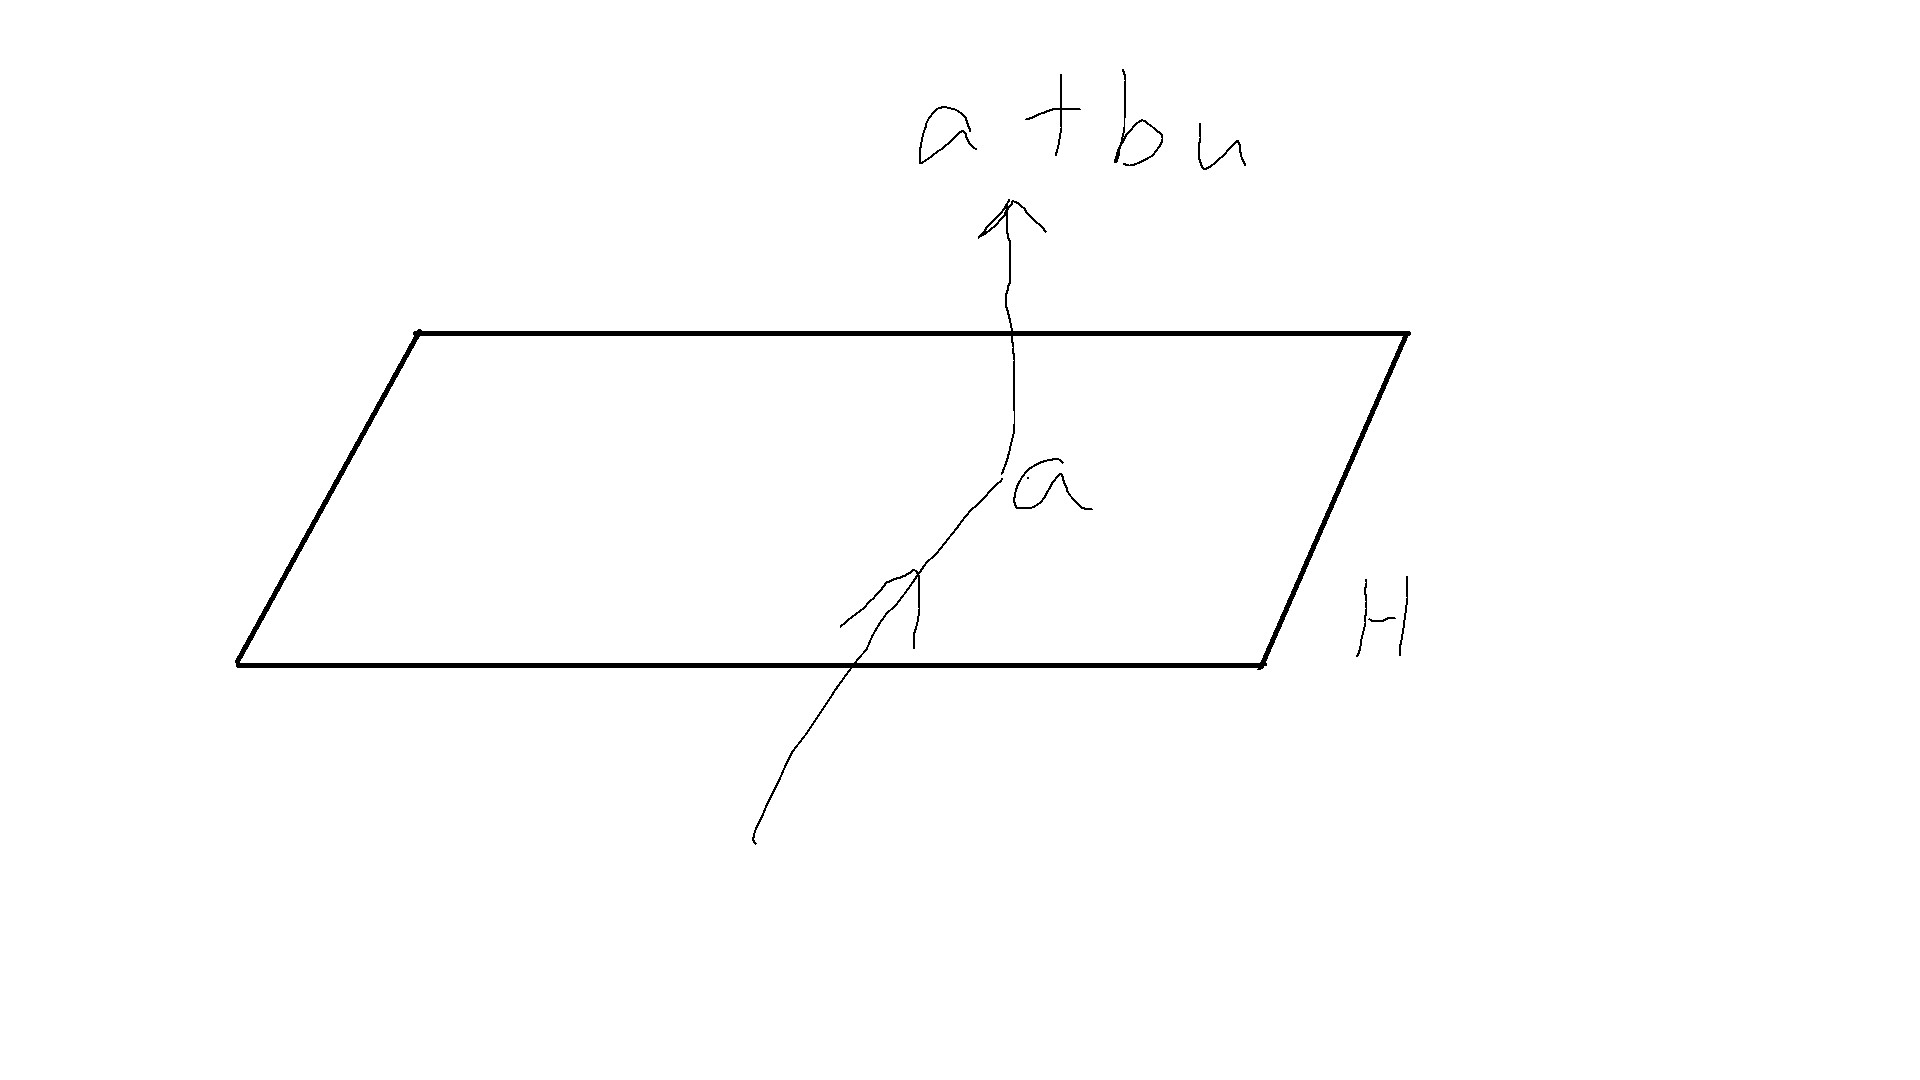
\includegraphics[scale=0.30]{Geometry_01}

\begin{equation*}
\begin{aligned}
H=\{x \in \R^n: u \cdot x = c\}
\end{aligned}
\end{equation*}
where $||u||=1$, $c \in \R$ is a given constant.

Reflection in $H$:
\begin{equation*}
\begin{aligned}
R_H: x \to x-2(x\cdot u-c)u
\end{aligned}
\end{equation*}
is an isometry (see example sheet).

Observe: if $x \in H$ then $R_H = x$.

If $a \in H$, $t \in \R$, then
\begin{equation*}
\begin{aligned}
R_H(a+tu) &= (a+tu)-2((a+tu)\cdot u-c)u\\
&=(a+tu)-2tu\\
&=a-tu
\end{aligned}
\end{equation*}
That means $R_H$ fixes precisely the points in $H$.

Conversely, suppose $S \in \Isom(\R^n)$ and $S$ fixes $H$.

Given $a \in H$, define translation by $a$: $T_a(x) = x+a$. Then set
\begin{equation*}
\begin{aligned}
R= T_{-a}ST_a \in \Isom(\R^n)
\end{aligned}
\end{equation*}
$R$ fixes $H' = T_{-a}(H)$ by inspection. Notice $0 \in H'$, so $H'$ is a vector subspace of $\R^n$.

If $H=\{x \cdot u = c\}$, then $H' = \{x \cdot u = 0\}$.

Then, whenever $x \in H'$, we have
\begin{equation*}
\begin{aligned}
(Ru,x) &= (Ru,Rx)\\
&= (u,x)\\
&=0
\end{aligned}
\end{equation*}
So $Ru \perp H'$, i.e. $Ru = \lambda u$ for some $\lambda \in \R$.

But $||Ru||^2 = 1$ as $||u||^2=1$, so $\lambda^2 = 1$, i.e. $\lambda = \pm 1$.

Since $R$ fixes $0$ ($0 \in H'$), $R$ is a linear map by Theorem 1.1 and either $R = id_{R^n}$ or $R=R_{H'}$ (corresponding to the matrix $\Diag(-1,1,...,1)$).

So $S$ is either $id_{\R^n}$ or $S=T_a R_{H'} T_{-a}$ is a reflection.

Checking $S$ when 

\begin{equation*}
\begin{aligned}
\lambda = -1: x \to x-a \to (x-a) - 2 ((x-a) \cdot u) u \to x - 2(x \cdot u - c) u
\end{aligned}
\end{equation*}
noting $a \cdot u = c$. Thus $S =R_H$.
\end{eg}

We find that $R_H$ is the unique isometry of $\R^n$ which fixes $H$ but is not identity.

It can be shown that every isometry of $\R^n$ is a composition of at most $n+1$ reflections (example sheet 1).

From Theorem 1.1, the subgroup consisting of isometries fixing the origin is $\{f(x)=Ax : AA^T = I\}$ is naturally isomorphic to $O(n)$.

$A \in O(n) \implies (\det A)^2 = 1 \implies \det A = \pm 1$.

\begin{defi}
The \emph{special orthogonal group}, $SO(n)$, consists of the matrices in $O(n)$ with determinant $+1$.
\end{defi}

\subsection{Orthogonal groups}

\begin{equation*} \tag{*}
\begin{aligned}
A= (\begin{matrix}
a & b\\
c & d
\end{matrix}) \iff a^2+c^2 = 1, b^2+d^2 =1 , ab+cd = 0 \iff A \in O(2).
\end{aligned}
\end{equation*}
Set $a = \cos \theta$, $b = -\sin \varphi$, $c = \sin \theta$, $d=\cos\varphi$ for appropriate $0 \leq \theta,\varphi \leq 2\pi$. So (*) says $\tan\theta = \tan \varphi \in \R \cup \{ \infty\}$. So $\theta = \varphi$ or $\theta = \varphi \pm \pi$. Respectively, 
\begin{equation*}
\begin{aligned}
A=\left(\begin{matrix}
\cos\theta & -\sin\theta\\
\sin\theta & \cos\theta
\end{matrix}\right)
\end{aligned}
\end{equation*}
is a rotation through $\theta$ about $O$. $\det A=1$, so $A \in SO(2)$. The other possibility is
\begin{equation*}
\begin{aligned}
A = \left(\begin{matrix}
\cos\theta & \sin\theta\\
\sin\theta & -\cos\theta
\end{matrix}\right)
\end{aligned}
\end{equation*}
fixes a line $l$ and must be a reflection in $l$ (see graph below). We have $\det A = -1$.

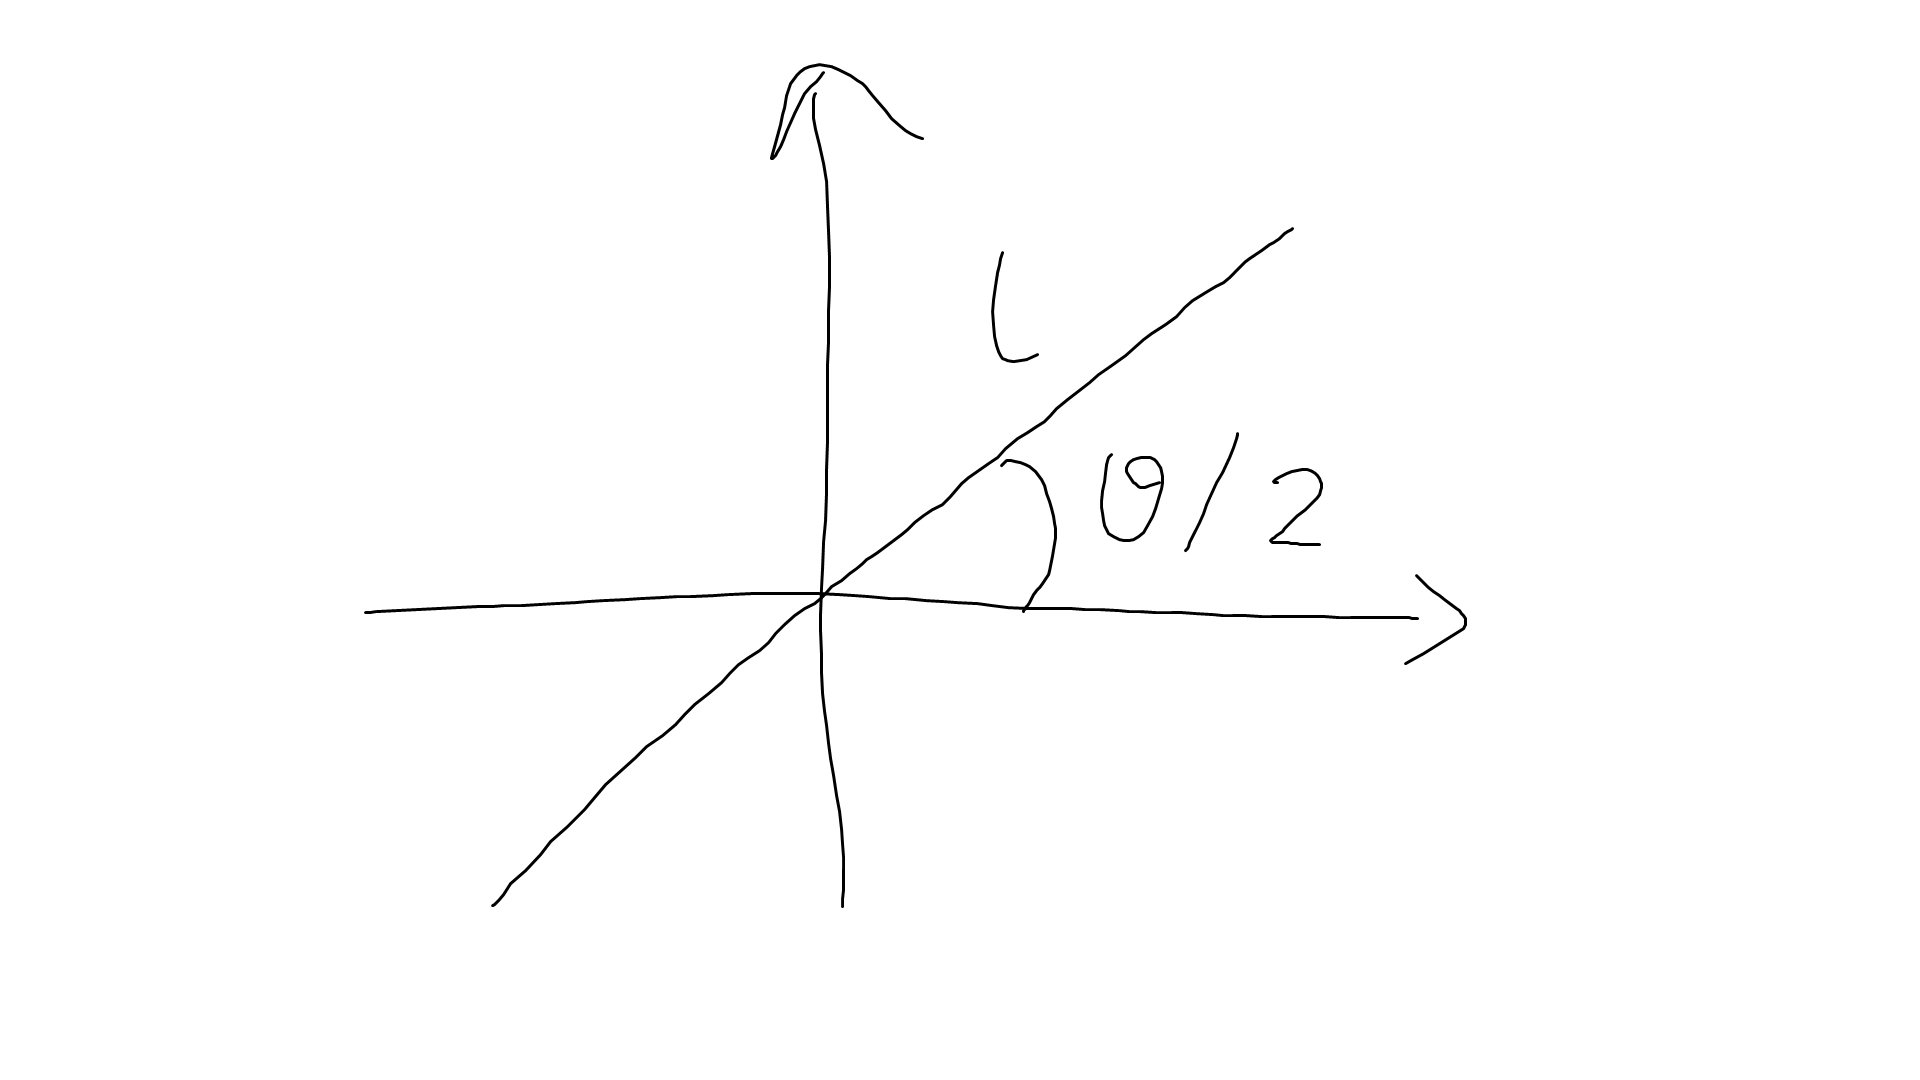
\includegraphics[scale=0.3]{Geometry_02}


\begin{rem}
\emph{Orientation} of a vector space on equivalence class of bases.

$\bullet$ Let $v_1,...,v_n$ and $v'_1,...,v'_n$ and $A=(A_{ij})$ the respective matrix for change from $\{v_i\}$ to $\{v'_i\}$. Then the bases are "equivalent", i.e. have the same orientation iff $\det A >0$.

We define an isometry $f(x)=Ax+b$ to be \emph{orientation-preserving} if $\det A = 1$, \emph{orientaiton-reversing} if $\det A = -1$.
\end{rem}

Now we consider the group $O(3)$.

Consider first the case $\det A = 1$. Then
\begin{equation*}
\begin{aligned}
\det(A-I) = \det(A^T-I) = \det(A(A^T-I)) = \det(I-A)
\end{aligned}
\end{equation*}
But $A$ has dimension 3. So $\det(A-I)=0$. So $+1$ is an eigenvalue of $A$. So $\exists v_1 \in \R^3$ (WLOG let $||v_1|| = 1$) s.t. $Av_1 = v_1$.

Set $W = \left<v_1\right>^\perp$. Then
\begin{equation*}
\begin{aligned}
w \in W \implies (Aw,v_1)=(Aw,Av_1) = (w,v_1) = 0
\end{aligned}
\end{equation*} 
So $A|_W$ is a rotation of $2$-dimensional space $W$. Choose an orthonormal basis $\{v_2,v_3\}$ of $W$. Then w.r.t $\{v_1,v_2,v_3\}$, $A$ becomes
\begin{equation*}
\begin{aligned}
\left(\begin{matrix}
1 & 0 & 0\\
0 & \cos\theta & -\sin\theta\\
0 & \sin\theta & \cos\theta
\end{matrix}\right)
\end{aligned}
\end{equation*}

Now let $\det A = -1$. Then $-A$ has determinant $1$, so is of the above form in some orthonormal basis. So $A$ takes the form
\begin{equation*}
\begin{aligned}
\left(\begin{matrix}
-1 & 0 & 0\\
0 & \cos\varphi & -\sin\varphi\\
0 & \sin\varphi & \cos\varphi
\end{matrix}\right)
\end{aligned}
\end{equation*}
with $\varphi = \theta + \pi$. This is a \emph{rotated reflection} (pure reflection when $\phi = 0$).

\subsection{Curves in $\R^n$}
\begin{defi}
A \emph{curve} $\Gamma$ in $\R^n$ is a continuous function $\Gamma: [a,b] \to \R^n$.

A dissection is $\mathcal{D}:a = t_0<t_1<...<t_N = b$ of $[a,b]$.

Set $P_i = \Gamma(t_i) \in \R^n$, $S_\mathcal{D} = \sum_i ||\vec{P_i P_{i+1}}||$.

We define the \emph{length} of $\Gamma$ as
\begin{equation*}
\begin{aligned}
l=\sup_\mathcal{D} S_\mathcal{D}
\end{aligned}
\end{equation*}
if this exists (i.e. finite).

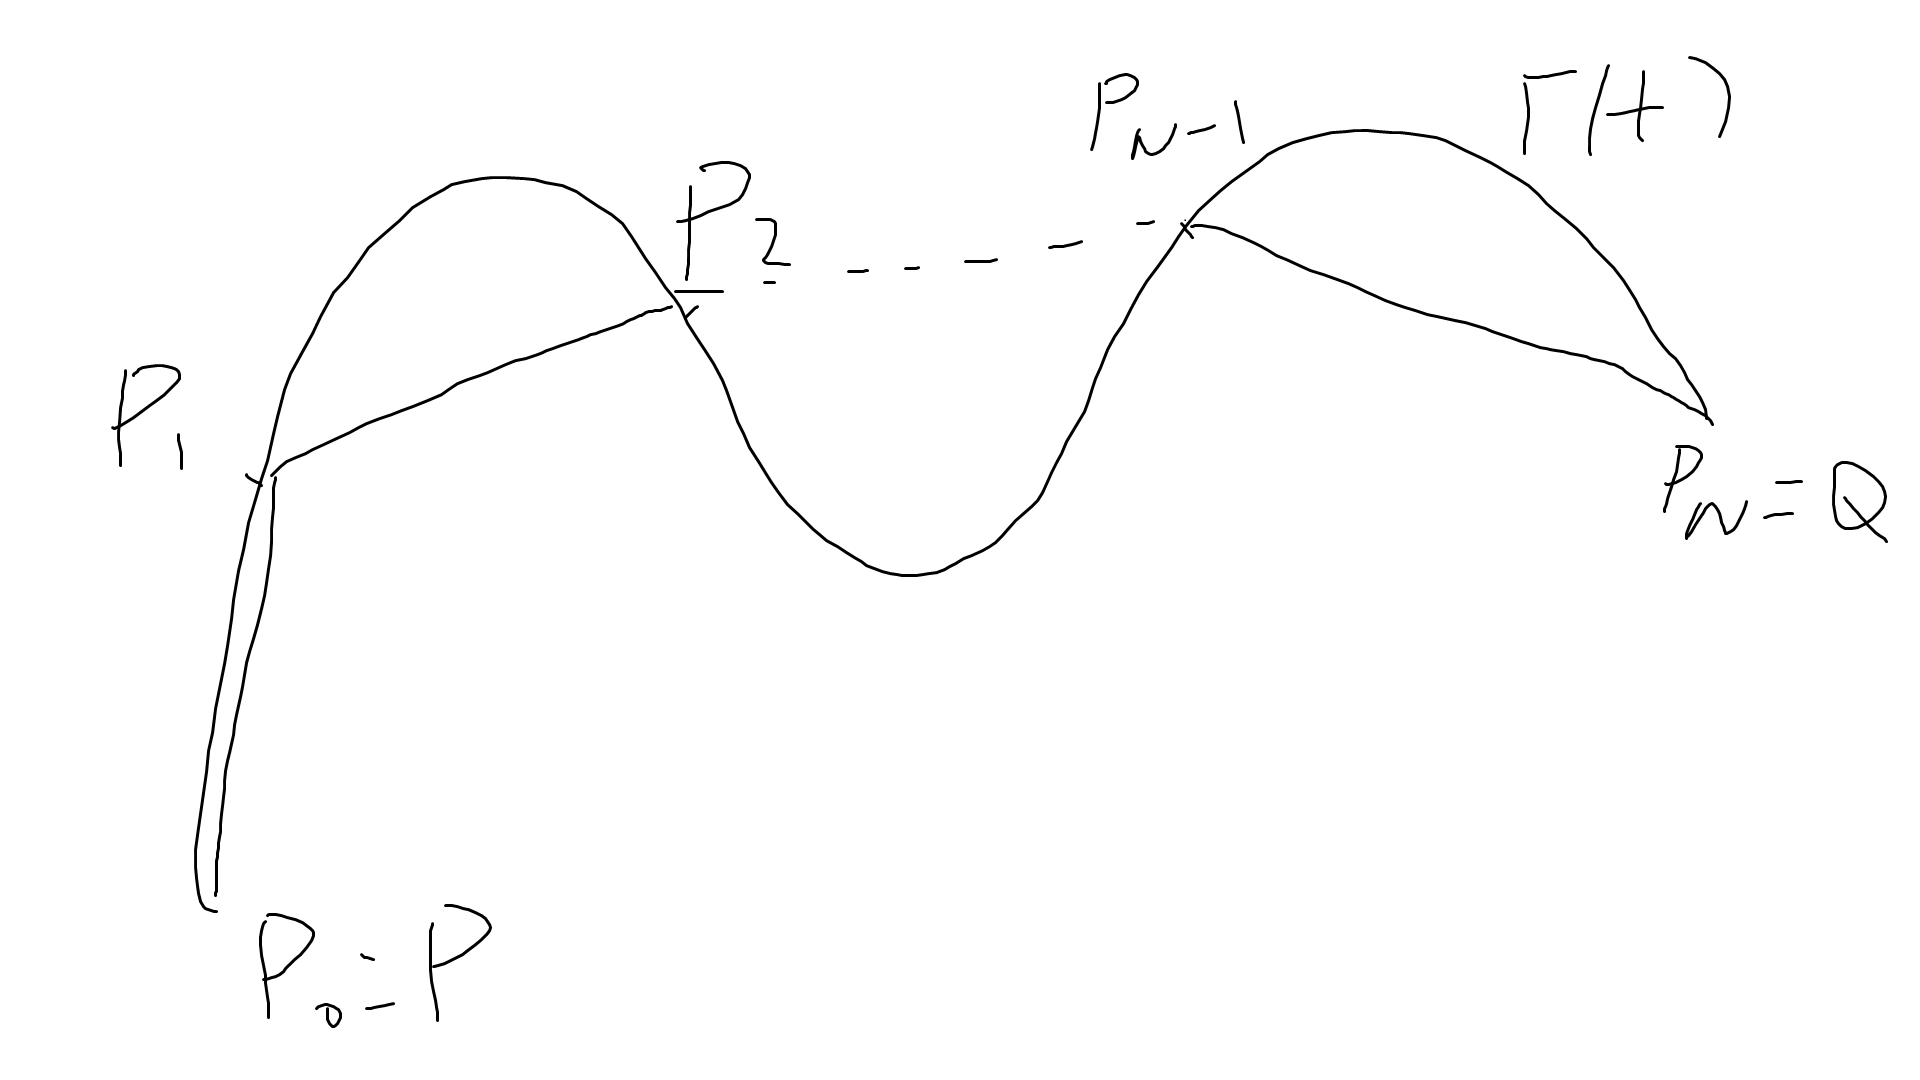
\includegraphics[scale=0.4]{Geometry_03}

If $\mathcal{D} = (P_i = \Gamma(t_i))_{i=1}^N$ is a dissection of $\Gamma$ and $\mathcal{D}'$ is a refinement (contain extra points) of $\mathcal{D}$, then $S_\mathcal{D} \leq S_\mathcal{D'}$ by triangle inequality.

Let $\Mesh(\mathcal{D}) = \max_i (t_i-t_{i-1})$. Then, if the length $l$ of $\Gamma$ exists (i.e. finite), then we have
\begin{equation*}
\begin{aligned}
l = \lim_{\Mesh(\mathcal{D} \to 0)} S_\mathcal{D}.
\end{aligned}
\end{equation*}

Note also $l = \min\{\tilde{l}: \tilde{l} \geq S_\mathcal{D} \forall \mathcal{D}\}$.

\end{defi}

\begin{prop} 1.2 \label{th1.2}\\
If $\Gamma$ is continuously differentiable ($C^1$), then the length of $\Gamma$ is
\begin{equation*}
\begin{aligned}
l = \int_a^b ||\Gamma'(t)||dt
\end{aligned}
\end{equation*}
\begin{proof}
Assume $n=3$ to ease the notation. We have
\begin{equation*}
\begin{aligned}
\Gamma(t) = (f_1(t),f_2(t),f_3(t)).
\end{aligned}
\end{equation*}
Given $s \neq t$ in $[a,b]$, use MVT for each $f_i$, we get
\begin{equation*}
\begin{aligned}
\frac{f_i(t)-f_i(s)}{t-s} = f'_i(\xi_i)
\end{aligned}
\end{equation*}
for some $\xi_i \in (s,t)$.

$f'_i$ is continuous on $[a,b]$. So $f'_i$ is uniformly continuous. So $\forall \varepsilon>0$, $\exists \delta = \delta(\varepsilon)>0$ s.t. $|t-s| < \delta \implies |f'_i(xi_i) - f'_i(\xi)| < \varepsilon$ $\forall \xi \in (s,t)$.

So 
\begin{equation*}
\begin{aligned}
||\frac{\Gamma(t) - \Gamma(s)}{t-s} - \Gamma'(\xi)|| &= ||(f'_1(\xi_1),f'_2(\xi_2),f'_3(\xi_3)) - (f'_1(\xi),f'_2(\xi),f'_3(\xi))||\\
&< \frac{\varepsilon}{3} + \frac{\varepsilon}{3} + \frac{\varepsilon}{3}\\
&= \varepsilon
\end{aligned}
\end{equation*}
i.e.
\begin{equation*}
\begin{aligned}
||\Gamma(t)-\Gamma(s)-(t-s)\Gamma'(\xi)|| < \varepsilon(t-s)
\end{aligned}
\end{equation*}
Now let $t=t_i,s=t_{i-1},\xi = \frac{t_{i-1}+t_i}{2}$. So
\begin{equation*}
\begin{aligned}
(t_i-t_{i-1}) ||\Gamma'(\frac{t_{i-1}+t_i}{2})|| -\varepsilon(t_i-t_{i-1}) &\leq ||\Gamma(t_i) - \Gamma(t_{i-1})|| \leq (t_i-t_{i-1}) ||\Gamma'(\frac{t_i+t_{i-1}}{2})|| + \varepsilon(t_i-t_{i-1})
\end{aligned}
\end{equation*}
So
\begin{equation*}
\begin{aligned}
\sum_i (t_i-t_{i-1}) ||\Gamma'(\frac{t_i+t_{i-1}}{2}||-\varepsilon(b-a) < S_\mathcal{D} < \sum_i (t_i-t_{i-1})||\Gamma'(\frac{t_i+t_{i-1}}{2})|| + \varepsilon(b-a)
\end{aligned}
\end{equation*}
But $||\Gamma'(t)||$ is continuous, hence integrable. So
\begin{equation*}
\begin{aligned}
\sum_i (t_i-t_{i-1})||\Gamma'(\frac{t_i+t_{i-1}}{2})|| \to \int_a^b ||\Gamma'(t)|| dt
\end{aligned}
\end{equation*}
as $\Mesh(\mathcal{D}) \to 0$.

Thus the length of $\Gamma$ is
\begin{equation*}
\begin{aligned}
l=\lim_{\Mesh(\mathcal{D}) \to 0} S_\mathcal{D} = \int_a^b ||\Gamma'(t)||dt.
\end{aligned}
\end{equation*}
\end{proof}
\end{prop}

\newpage

\section{Spherical Geometry}
Denote $S=S^2 \subset \R^3$ the unit sphere in with centre origin.

\begin{defi}
A \emph{great circle} a.k.a (spherical) line in $S^2$, is $S^2 \cap$ a plane through the origin.
\end{defi}

Given two distincts non-antipodal points $P,Q \in S^2$, there exists a unique line in $S^2$ through $P,Q$ (as $P,Q$ and the origin fix a plane).

\begin{defi}
For $P,Q \in S^2$, the distance $d(P,Q)$ is the length of the shorter of the two spherical line segments $PQ$ along the great circle through $P$ and $Q$. $d(P,Q) = \pi$ if $P,Q$ are antipodal.
\end{defi}

Note that $d(P,Q)$ $=$ angle between $\mathbf{P} = \vec{OP}$ and $\mathbf{Q} = \vec{OQ}$ $= \cos^{-1} (\mathbf{P} \cdot \mathbf{Q})$.

A \emph{spherical triangle} $ABC$ is defined like a Euclidean triangle, but with $AB,BC,CA$ line segments in $S^2$ with lengths $<\pi$.

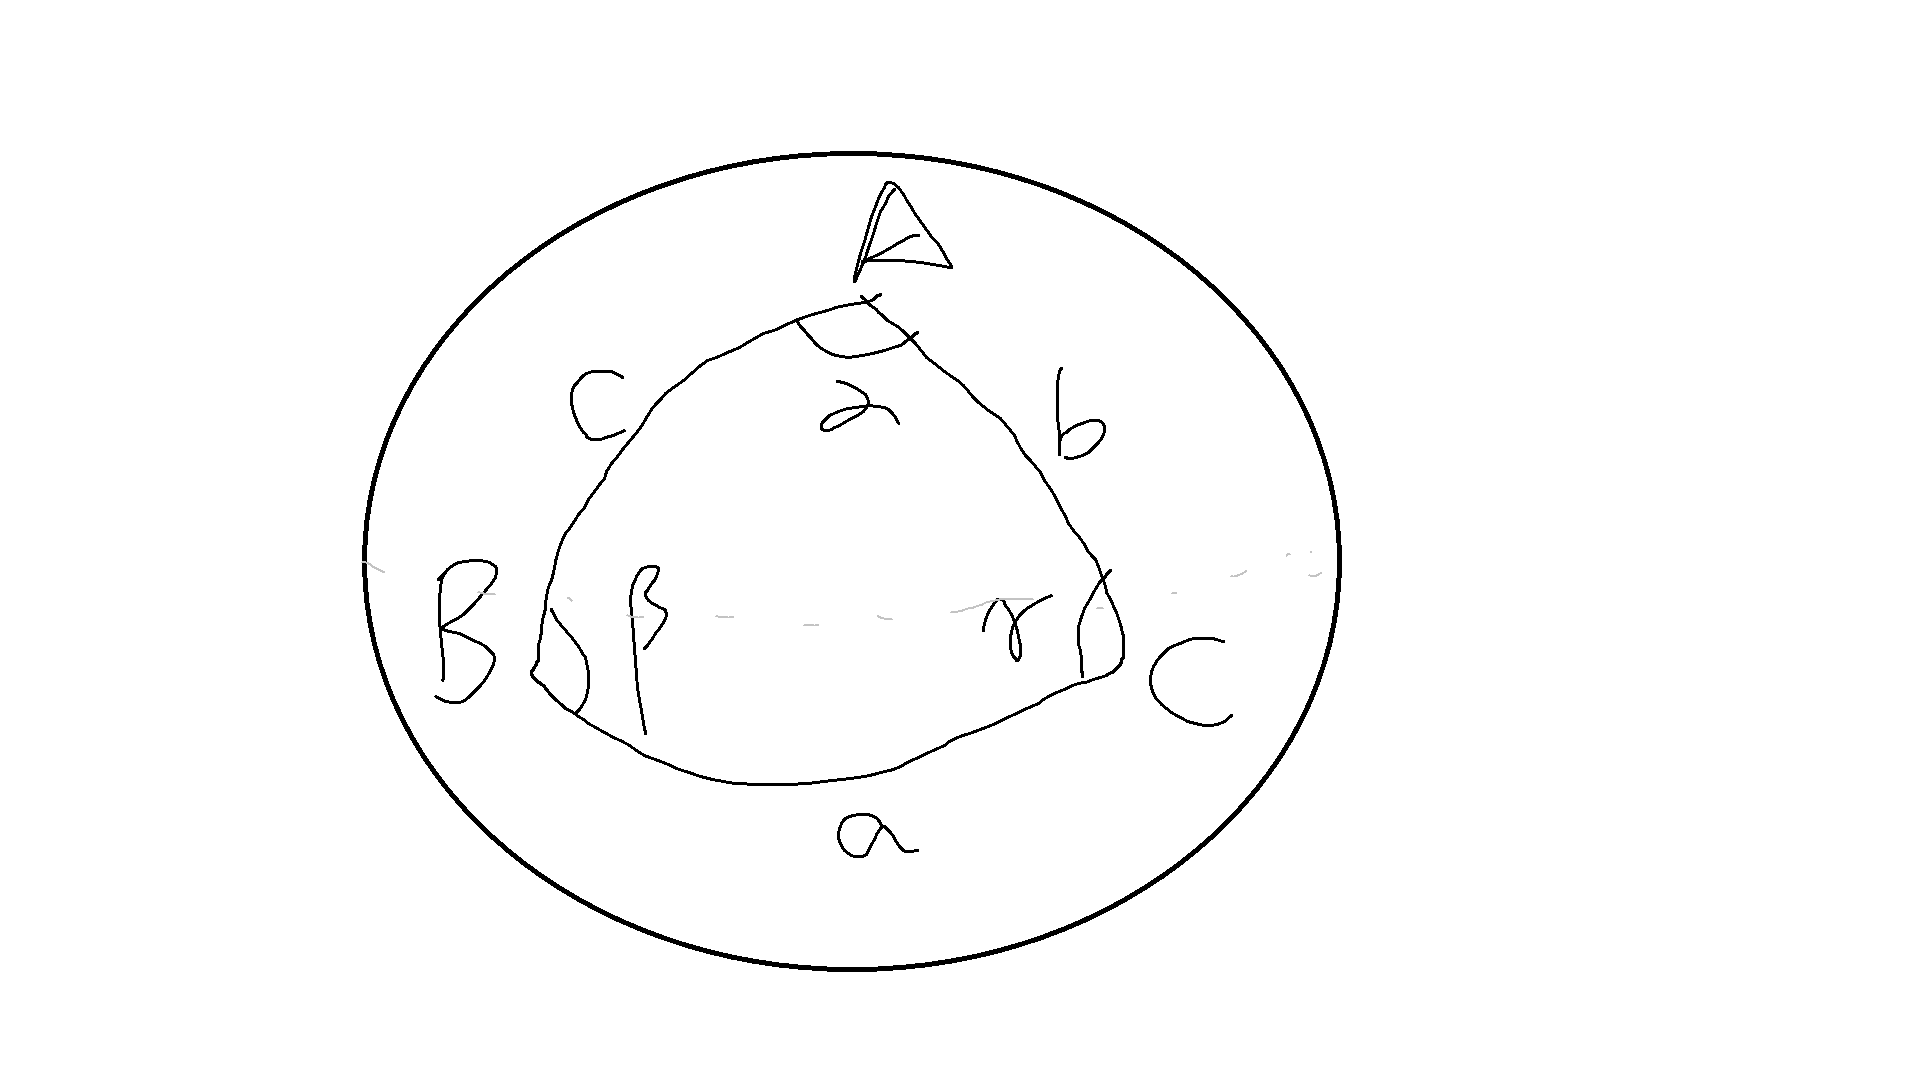
\includegraphics[scale=0.4]{Geometry_04}

\begin{notation}
Write $\mathbf{A} = \vec{OA}$ and etc.\\
Set
\begin{equation*}
\begin{aligned}
\mathbf{n}_1 = \frac{\mathbf{C} \times \mathbf{B}}{\sin a},\\
\mathbf{n}_2 = \frac{\mathbf{A} \times \mathbf{C}}{\sin b},\\
\mathbf{n}_3 = \frac{\mathbf{B} \times \mathbf{A}}{\sin c}.
\end{aligned}
\end{equation*}
These are unit normals to the planes $OBC,OCA,OAB$, pointing out of the solid $OABC$.

$\alpha,\beta,\gamma$ are the angle between planes defining respective sides of $ABC$.

Note $0<\alpha,\beta,\gamma < \pi$. So (angle between them)$\widehat{n_2,n_3} = \pi - \alpha$, $\mathbf{n}_2 \cdot \mathbf{n}_3 = -\cos \alpha$. Similarly, $\mathbf{n_1} \cdot \mathbf{n}_2 = -\cos \gamma$, $\mathbf{n}_1 \cdot \mathbf{n}_3 = -\cos \beta$.
\end{notation}

\begin{thm} 2.1 (Spherical cosine rule) \label{th2.1}\\
For a spherical triangle, we have
\begin{equation*}
\begin{aligned}
\sin a \sin b \cos \gamma = \cos c - \cos a \cos b.
\end{aligned}
\end{equation*}
\begin{proof}
Use $(\mathbf{C} \times \mathbf{B}) \cdot (\mathbf{A} \times \mathbf{C}) = (\mathbf{A} \cdot \mathbf{C}) (\mathbf{B} \cdot \mathbf{C}) - (\mathbf{C} \cdot \mathbf{C}) (\mathbf{B} \cdot \mathbf{A})$ and
\begin{equation*}
\begin{aligned}
\sum_k \varepsilon_{ijk} \varepsilon_{klm} = \delta_{il}\delta_{jm} - \delta_{im}\delta_{jl}
\end{aligned}
\end{equation*}
from vector calculus. We know $|\mathbf{C}| = 1$. So
\begin{equation*}
\begin{aligned}
RHS &= (\mathbf{A} \cdot \mathbf{C})(\mathbf{B} \cdot \mathbf{C}) - (\mathbf{B} \cdot \mathbf{A})
\end{aligned}
\end{equation*}
So
\begin{equation*}
\begin{aligned}
-\cos \gamma = \mathbf{n}_1 \cdot \mathbf{n}_2 = \frac{\mathbf{C} \times \mathbf{B}}{\sin a} \cdot \frac{\mathbf{A} \times \mathbf{C}}{\sin b} = \frac{(\mathbf{A} \cdot \mathbf{C}) (\mathbf{B}\cdot \mathbf{C}) - (\mathbf{A} \cdot \mathbf{B})}{\sin a \sin b} = \frac{\cos b \cos a - \cos c}{\sin a \sin b}
\end{aligned}
\end{equation*}
which is equivalent to what is required.
\end{proof}
\end{thm}

\begin{coro} 2.2 (Pythagoras for $S^2$) \label{th2.2} \\
If $\gamma = \frac{\pi}{2}$, then $\cos c = \cos a \cdot \cos b$.
\end{coro}

\begin{thm} 2.3 (Spherical sine rule) \label{th2.3}\\
For a spherical triangle, we have
\begin{equation*}
\begin{aligned}
\frac{\sin a}{\sin \alpha} = \frac{\sin b}{\sin \beta} = \frac{\sin c}{\sin \gamma}
\end{aligned}
\end{equation*}
\begin{proof}
Use
\begin{equation*}
\begin{aligned}
(\mathbf{A} \times \mathbf{C} ) \times (\mathbf{C} \times \mathbf{B}) = (\mathbf{C} \cdot (\mathbf{B} \times \mathbf{A})) \mathbf{C}
\end{aligned}
\end{equation*}
from vector calculus. Recall $\widehat{n_1,n_2} = \pi - \gamma$. We have
\begin{equation*}
\begin{aligned}
LHS &= -(\mathbf{n}_1 \times \mathbf{n}_2) \sin a \sin b
\end{aligned}
\end{equation*}
So $\mathbf{n}_1 \times \mathbf{n}_2 = \mathbf{C} \sin \gamma$, as from RHS we see that this is a multiple of $\mathbf{C}$. So
\begin{equation*}
\begin{aligned}
\mathbf{C} \cdot (\mathbf{A} \times \mathbf{B}) = \sin a \sin b \sin \gamma = \mathbf{A} \cdot (\mathbf{B} \times \mathbf{C}) = \sin b \sin c \sin \alpha
\end{aligned}
\end{equation*}
Multiply by $\frac{1}{\sin \alpha \sin \beta \sin \gamma}$ we get
\begin{equation*}
\begin{aligned}
\frac{\sin c}{\sin \gamma} = \frac{\sin b}{\sin \beta} = \frac{\sin a}{\sin \alpha}
\end{aligned}
\end{equation*}
\end{proof}
\end{thm}

We have seen cosine and sine rules for spherical triangles. There is a second cosine rule (Sheet 1 Q15).

\begin{rem}
Recall for small $a,b,c$, $\sin a = a + O(a^3)$, $\cos a = 1-\frac{a^2}{2} + O(a^4)$. We get the Euclidean versions in the limit $a,b,c \to 0$.

e.g. in Theorem 2.1,
\begin{equation*}
\begin{aligned}
ab\cos \gamma = 1-\frac{c^2}{2} - \left(1-\frac{a^2}{2}\right)\left(1-\frac{b^2}{2}\right) + O(||(a,b,c)||^3)\\
\implies c^2+2ab\cos\gamma = a^2+b^2+O(||(a,b,c)||^3).
\end{aligned}
\end{equation*}
\end{rem}

If $\gamma = \pi$, then $C$ is in the line segment $AB$. So $c=a+b$. Otherwise from Theorem 2.1, $\cos c > \cos a \cos b - \sin a\sin b = \cos(a+b)$, so $c<a+b$. Also $c<\pi,a+b<2\pi$.

\begin{coro} (Triangle inequality)\\
$\forall P,Q,R \in S^2$, we have $d(P,Q)+d(Q,R) \geq d(P,R)$ (spherical distance), with equality only if $Q$ is in the line segment $PR$ of the shorter length.
\begin{proof}
The only case not covered by the previous discussion is when $d(P,R) = \pi$, i.e. $P,R$ antipodal. Then $R$ is in the line $PQ$. So $d(P,R)=d(P,Q)+d(Q,R)$.
\end{proof}
\end{coro}

So we find that $(S^2,d)$ is a \emph{metric space}.

\begin{prop} 2.5\\
Given a curve $\Gamma$ on $S^2$ from $P$ to $Q$ with $l=length(\Gamma)$, we have
\begin{equation*}
\begin{aligned}
l \geq d(P,Q)
\end{aligned}
\end{equation*}
Moreover, if $l=d(P,Q)$ then $\Gamma$ is a spherical line segment.
\begin{proof}
$\Gamma:[0,1] \to S^2$. $length(\Gamma)=l$ $\implies$ $\forall$ dissection $\mathcal{D}$ of $[0,1]$: $0=t_0<t_1<...<t_N = 1$, $p_i = \Gamma(t_i)$,
\begin{equation*}
\begin{aligned}
\tilde{\mathcal{S}_\mathcal{D}} := \sum_{i=1}^N d(p_{i-1},p_i) > \mathcal{S}_\mathcal{D} = \sum_{i=1}^N |\vec{p_{i-1}p_i}|
\end{aligned}
\end{equation*}
where RHS is $\R^3$ distance.

Using the fact $\sin \theta < \theta$ $\forall \theta >0$,

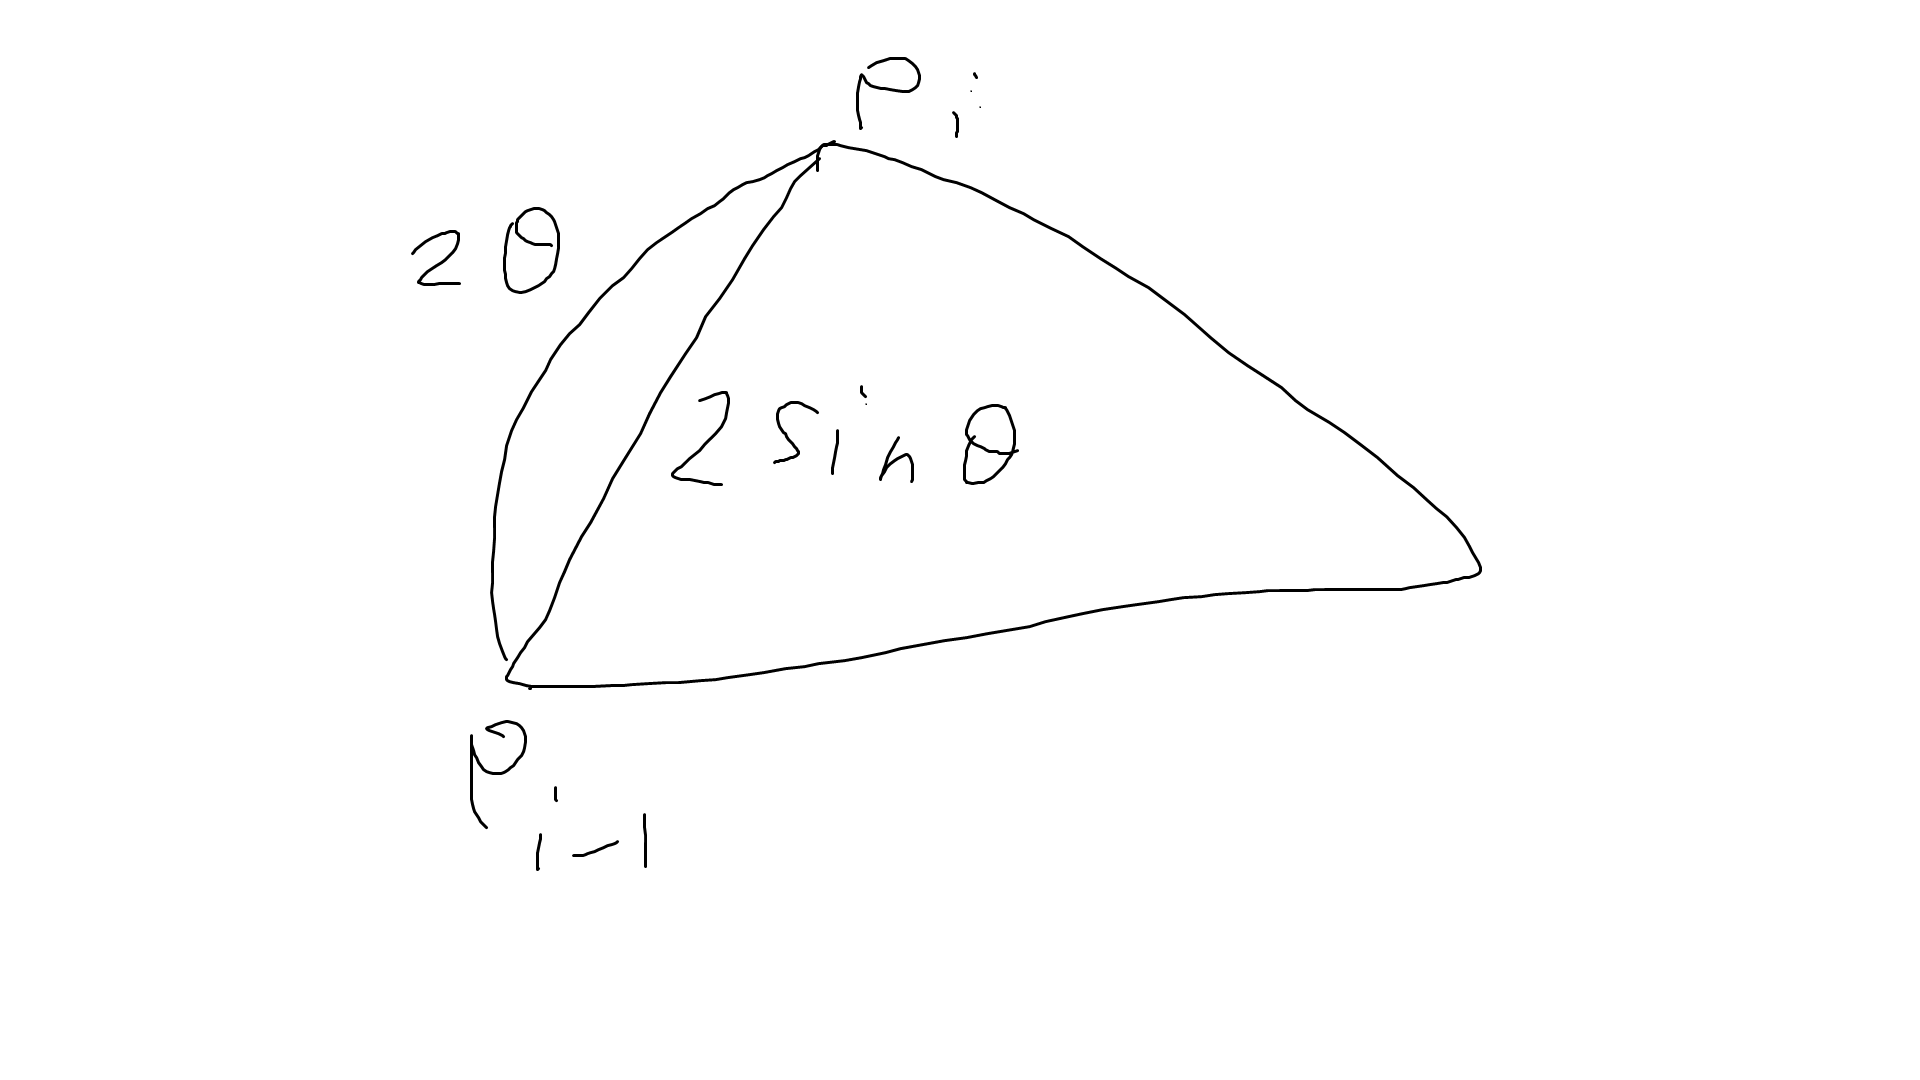
\includegraphics[scale=0.4]{Geometry_05}

Now suppose $l<d(P,Q)$. Then we can choose $\varepsilon>0$ s.t. $(1+\varepsilon)l < d(P,Q)$. Now since $\frac{\sin\theta}{\theta} \to 1$ as $\theta \to 0$, $2\theta \leq (1+\varepsilon)2\sin\theta$ for small $\theta > 0$.

$\Gamma$ is uniformly continuous on $[0,1]$. So we can choose a refined $\mathcal{D}$ with $d(p_{i-1},p_i) \leq (1+\varepsilon) |\vec{p_{i-1}p_i}|$. So
\begin{equation*}
\begin{aligned}
\tilde{\mathcal{S}}_\mathcal{D} \leq (1+\varepsilon)\mathcal{S}_\mathcal{D} \leq (1+\varepsilon)l < d(P,Q)
\end{aligned}
\end{equation*}
But $\tilde{\mathcal{S}_\mathcal{D}} \geq d(P,Q)$ by triangle inequality (applied many times). Contradiction. So $l \geq d(P,Q)$.

Suppose now $l=d(P,Q)$ for some $\Gamma:[0,1] \to S$. Then $\forall t \in [0,1]$, 
\begin{equation*}
\begin{aligned}
d(P,Q) = l &= length \Gamma|_{[0,t]} + length \Gamma|_{[t,1]}\\
&\geq d(P,\Gamma(t)) + d(\Gamma(t),Q)
\end{aligned}
\end{equation*}
So $d(P,Q) = d(P,\Gamma(t)) + d(\Gamma(t,Q)$ $\forall t$. So $\Gamma(t)$ is in the shorter spherical line segment $PQ$.
\end{proof}
\end{prop}

Sheet 1 Q4 is the Euclidean version of this discussion.

\begin{rem}
If $\Gamma$ is a curve in $S^2$ of minimal length from $P$ to $Q$, then $\Gamma$ is a spherical line segment. Further, from the proof of proposition 2.5, $length(\Gamma|_{[0,t]}) = d(P,\Gamma(t))$ $\forall t \in [0,1]$. So the parameterisation of $\Gamma$ is \emph{monotonic}, i.e. the distance increases as $t$ increases.
\end{rem}

\begin{prop} 2.6 (Gauss-Bonnet theorem for $S^2$)\\
If $\Delta$ is a spherical triangle with angles $\alpha,\beta,\gamma$, then 
\begin{equation*}
\begin{aligned}
area(\Delta) = (\alpha+\beta+\gamma)-\pi.
\end{aligned}
\end{equation*}
\begin{proof}
A \emph{double lune} with angle $0<\alpha<\pi$ is two regions on $S$ cut out by 2 planes through antipodal points, say $A$ and $A'$, where $\alpha$ is the angle between the plane.

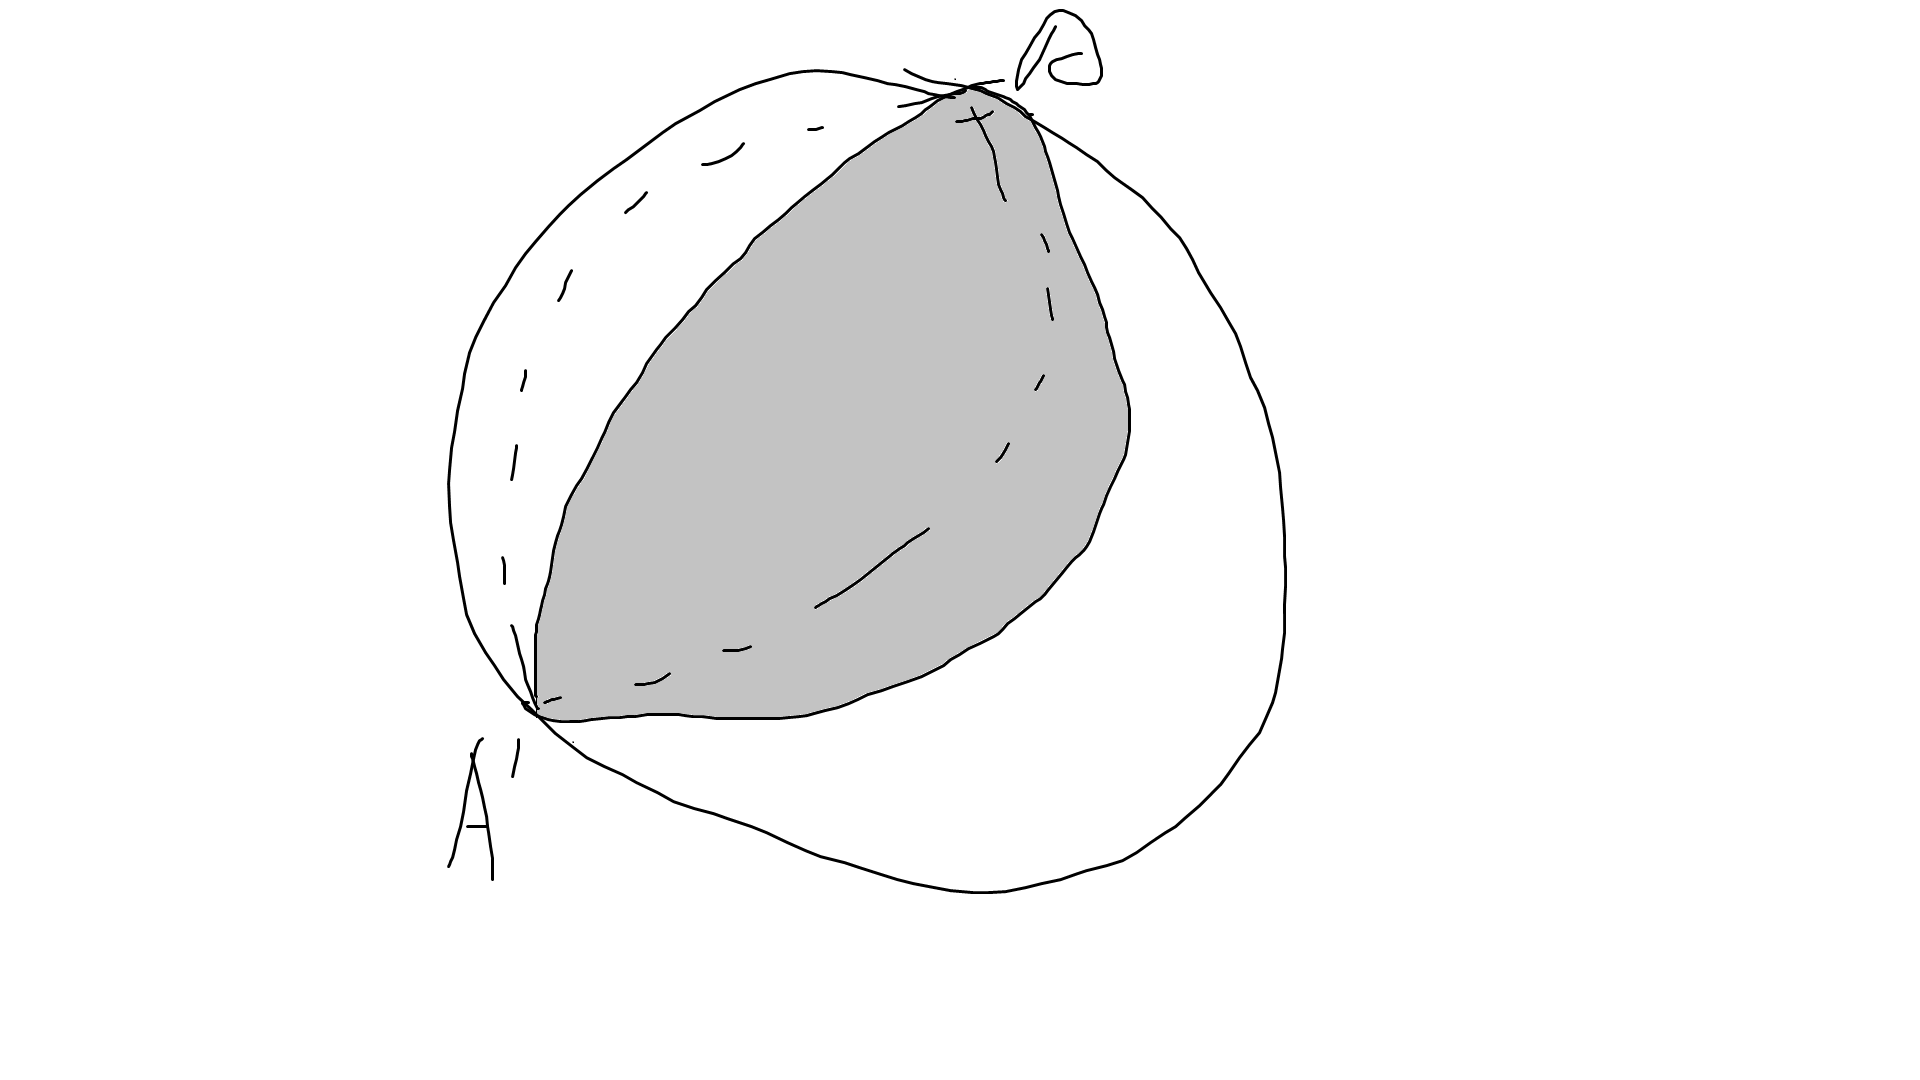
\includegraphics[scale=0.4]{Geometry_06}

The area of double lune is $4\alpha$ (noting it is proportional to $\alpha$, and $area(S^2) = 4\pi$).

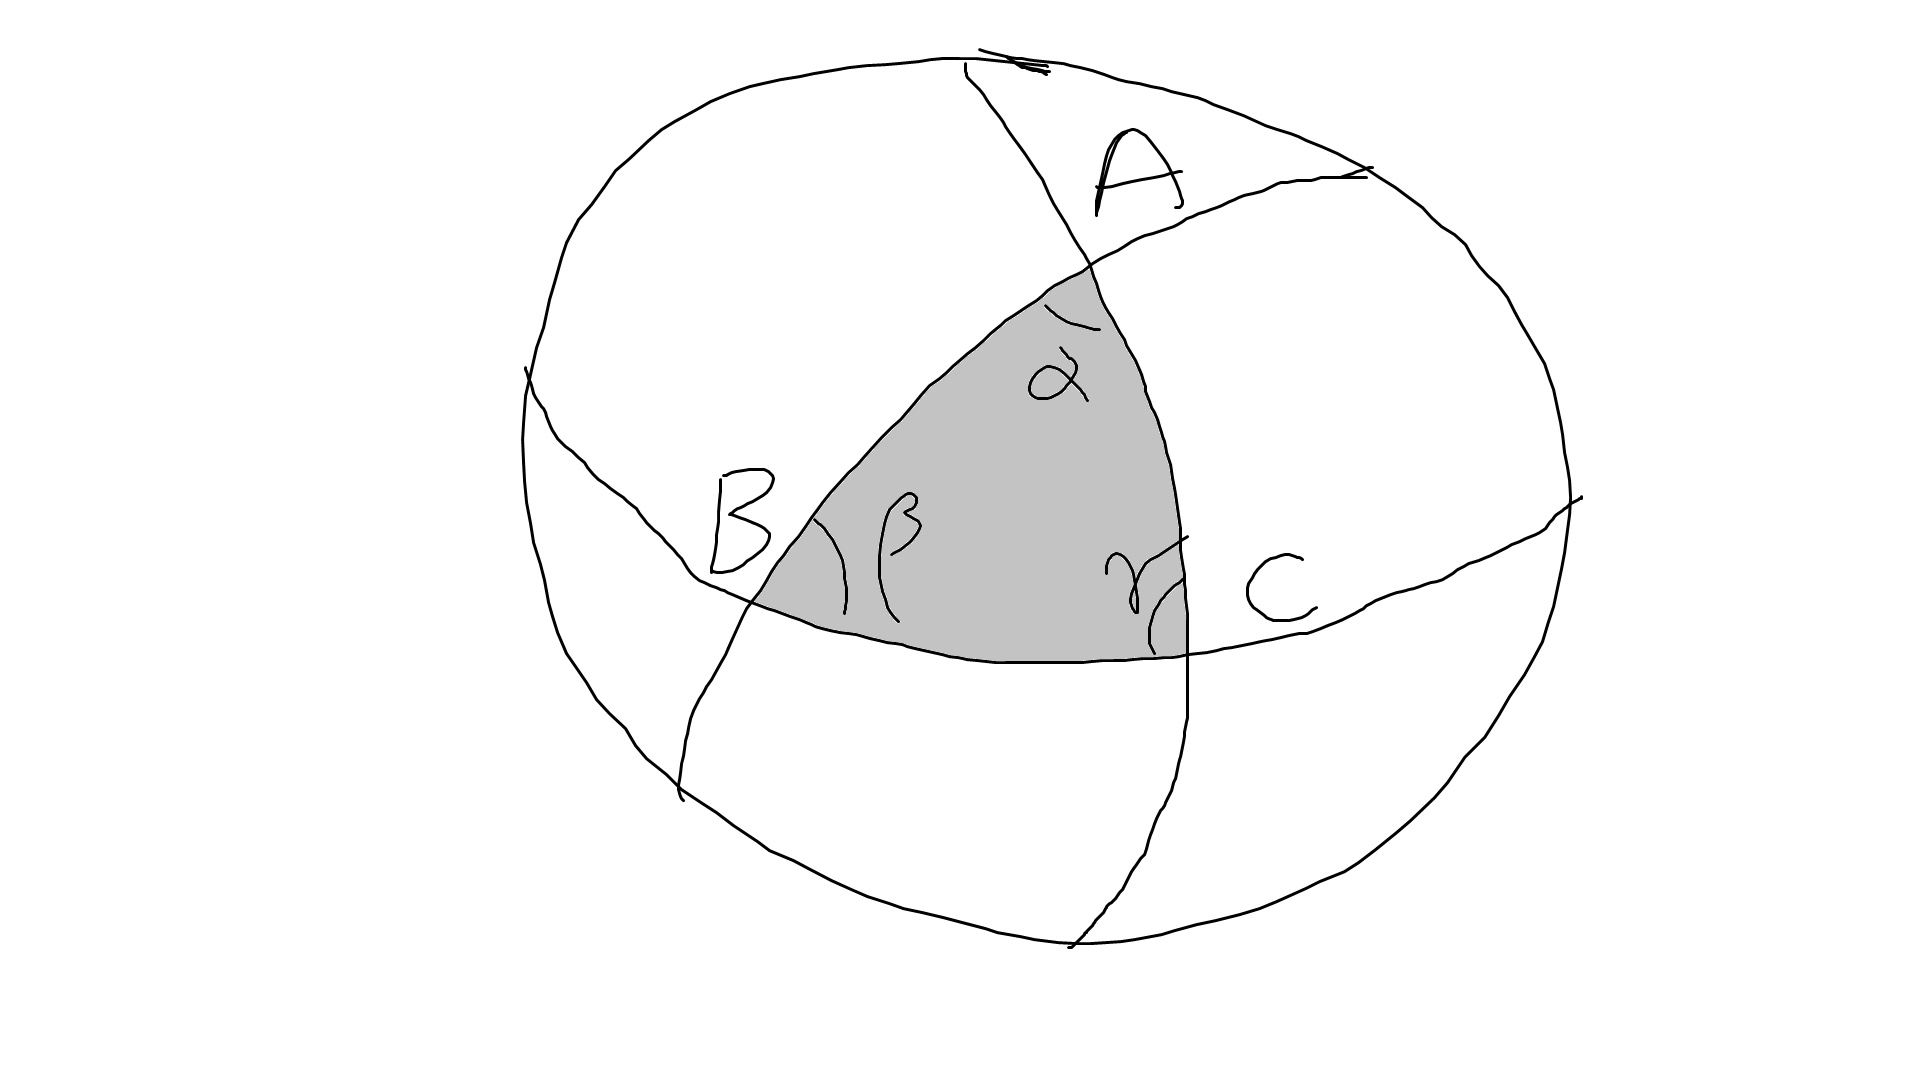
\includegraphics[scale=0.4]{Geometry_07}

$\Delta = ABC$ is the intersection of 3 single lunes. So $\Delta$ and its antipodal $\Delta'$ is a subset of each of 3 double lunes with angles $\alpha,\beta,\gamma$.

Any other $P \not\in \Delta \cup \Delta'$ is in only one double lune.

Thus $4(\alpha+\beta+\gamma) = 4\pi + 2\cdot (2\Delta)$ which gives the desired result.
\end{proof}
\end{prop}

\begin{rem}
(i) On $S$, we have $\alpha+\beta+\gamma>\pi$ ($\to \pi$ as $a,b,c \to 0$). \\
(ii) For convex $n$-gon, $area(M) = \sum_{i=1}^n \alpha_i - (n-2)\pi$ (cut into triangles).
\end{rem}

\subsection{M$\ddot{o}$bius geometry}
Consider $\C_\infty = \C \cup \{\infty\}$ with coordinates $\zeta=x+iy$.\\
The stereographic projection $\pi:S^2 \to \C_\infty$:

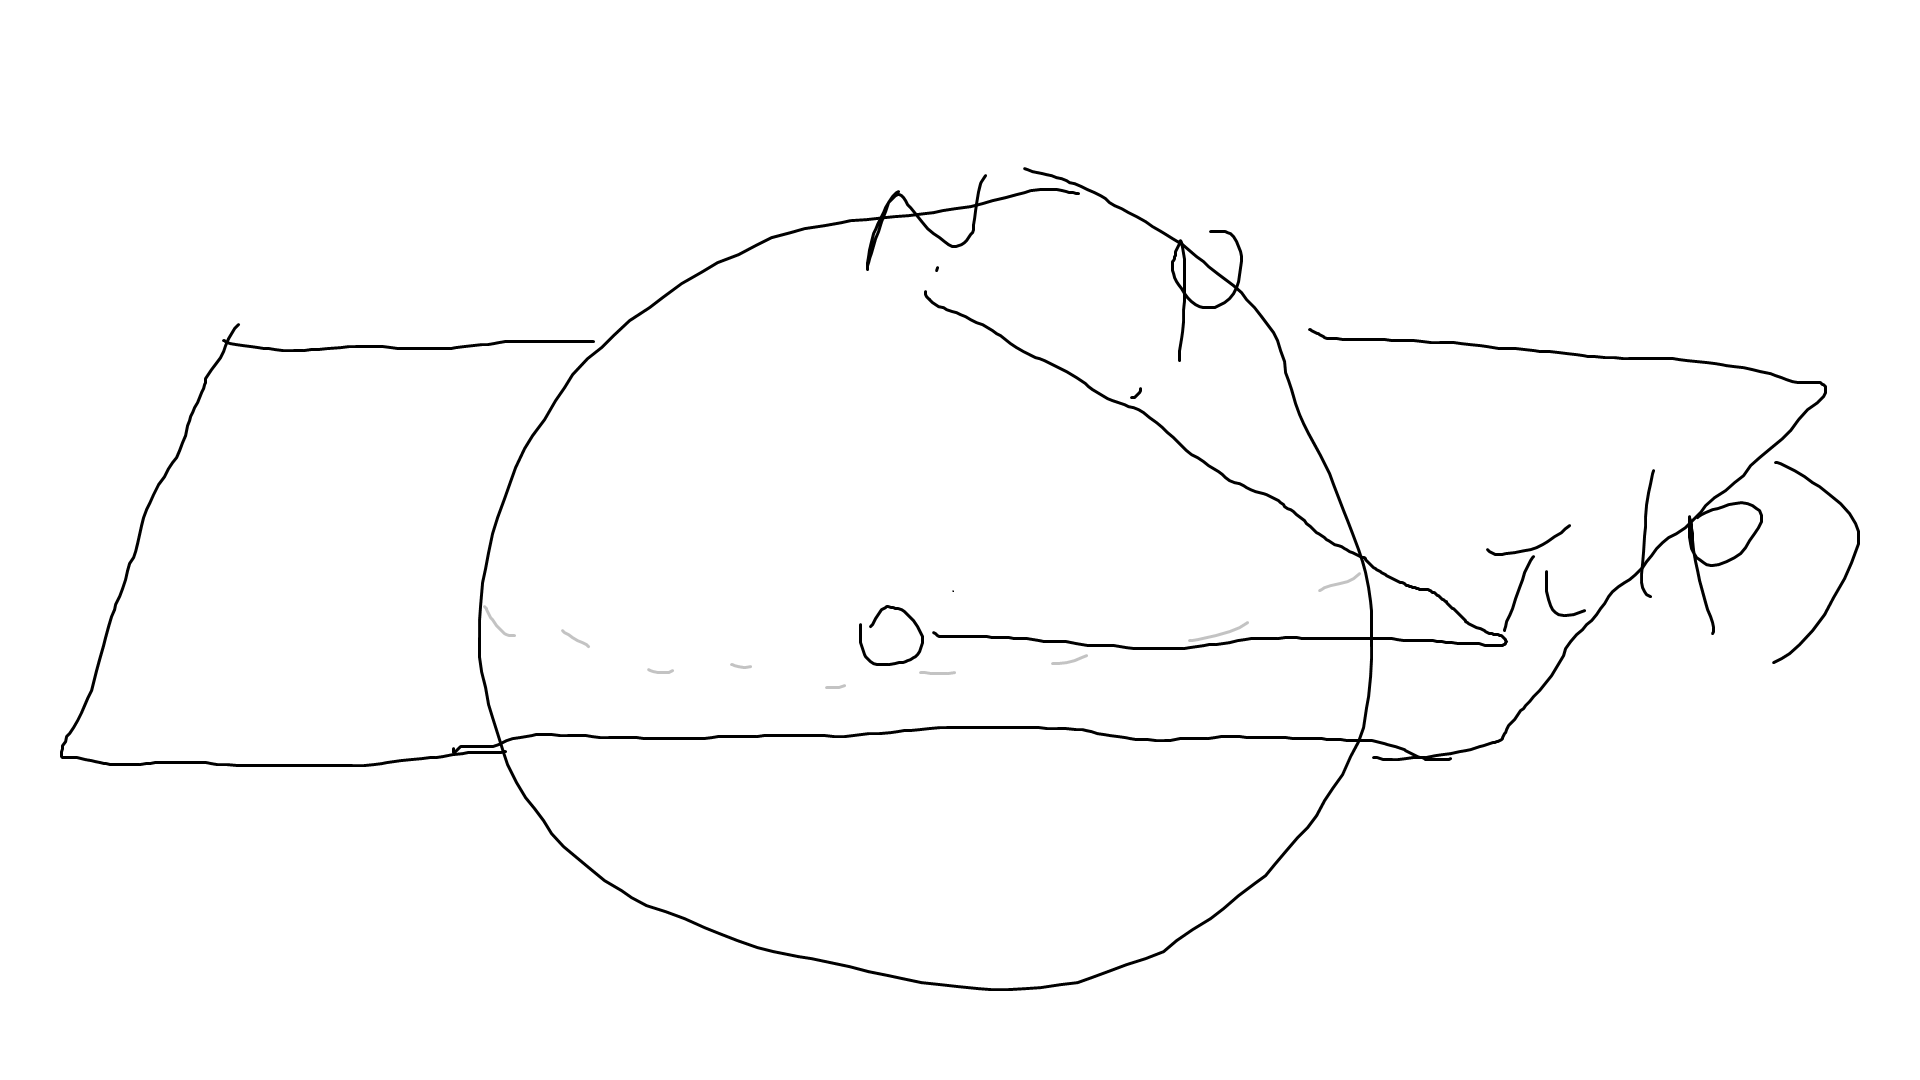
\includegraphics[scale=0.4]{Geometry_08}

is $\pi(P) = (NP) \cap \{z=0\} \cong \C \cong \R^2$, $\pi(N) =\infty$ where $N=(0,0,1)$.

By Euclidean geometry we can get
\begin{equation*}
\begin{aligned}
\pi(x,y,z) = \frac{x+iy}{1-z}
\end{aligned}
\end{equation*}

\begin{lemma} 2.7\\
If $\pi'$ is the stereographic projection from $(0,0,-1)$ (South pole), then
\begin{equation*}
\begin{aligned}
\pi'(P) = \frac{1}{\overline{\pi(P)}}
\end{aligned}
\end{equation*}
$\forall P \in S^2$.
\begin{proof}
Let $P=(x,y,z)$. Then $\pi(P) = \frac{x+iy}{1-z}$, $\pi'(P) = \frac{x+iy}{1+z}$. So
\begin{equation*}
\begin{aligned}
\overline{\pi(P)} \cdot \pi'(P) = \frac{x^2+y^2}{1-z^2} = 1
\end{aligned}
\end{equation*}
\end{proof}
\end{lemma}

Note: $\pi' \circ \pi^{-1}: \C \to \C$ takes $\zeta$ to $\frac{1}{\overline{\zeta}}$, the \emph{inversion in the unit circle} $\{x^2+y^2=1\} = \{|\zeta| = 1\}$.

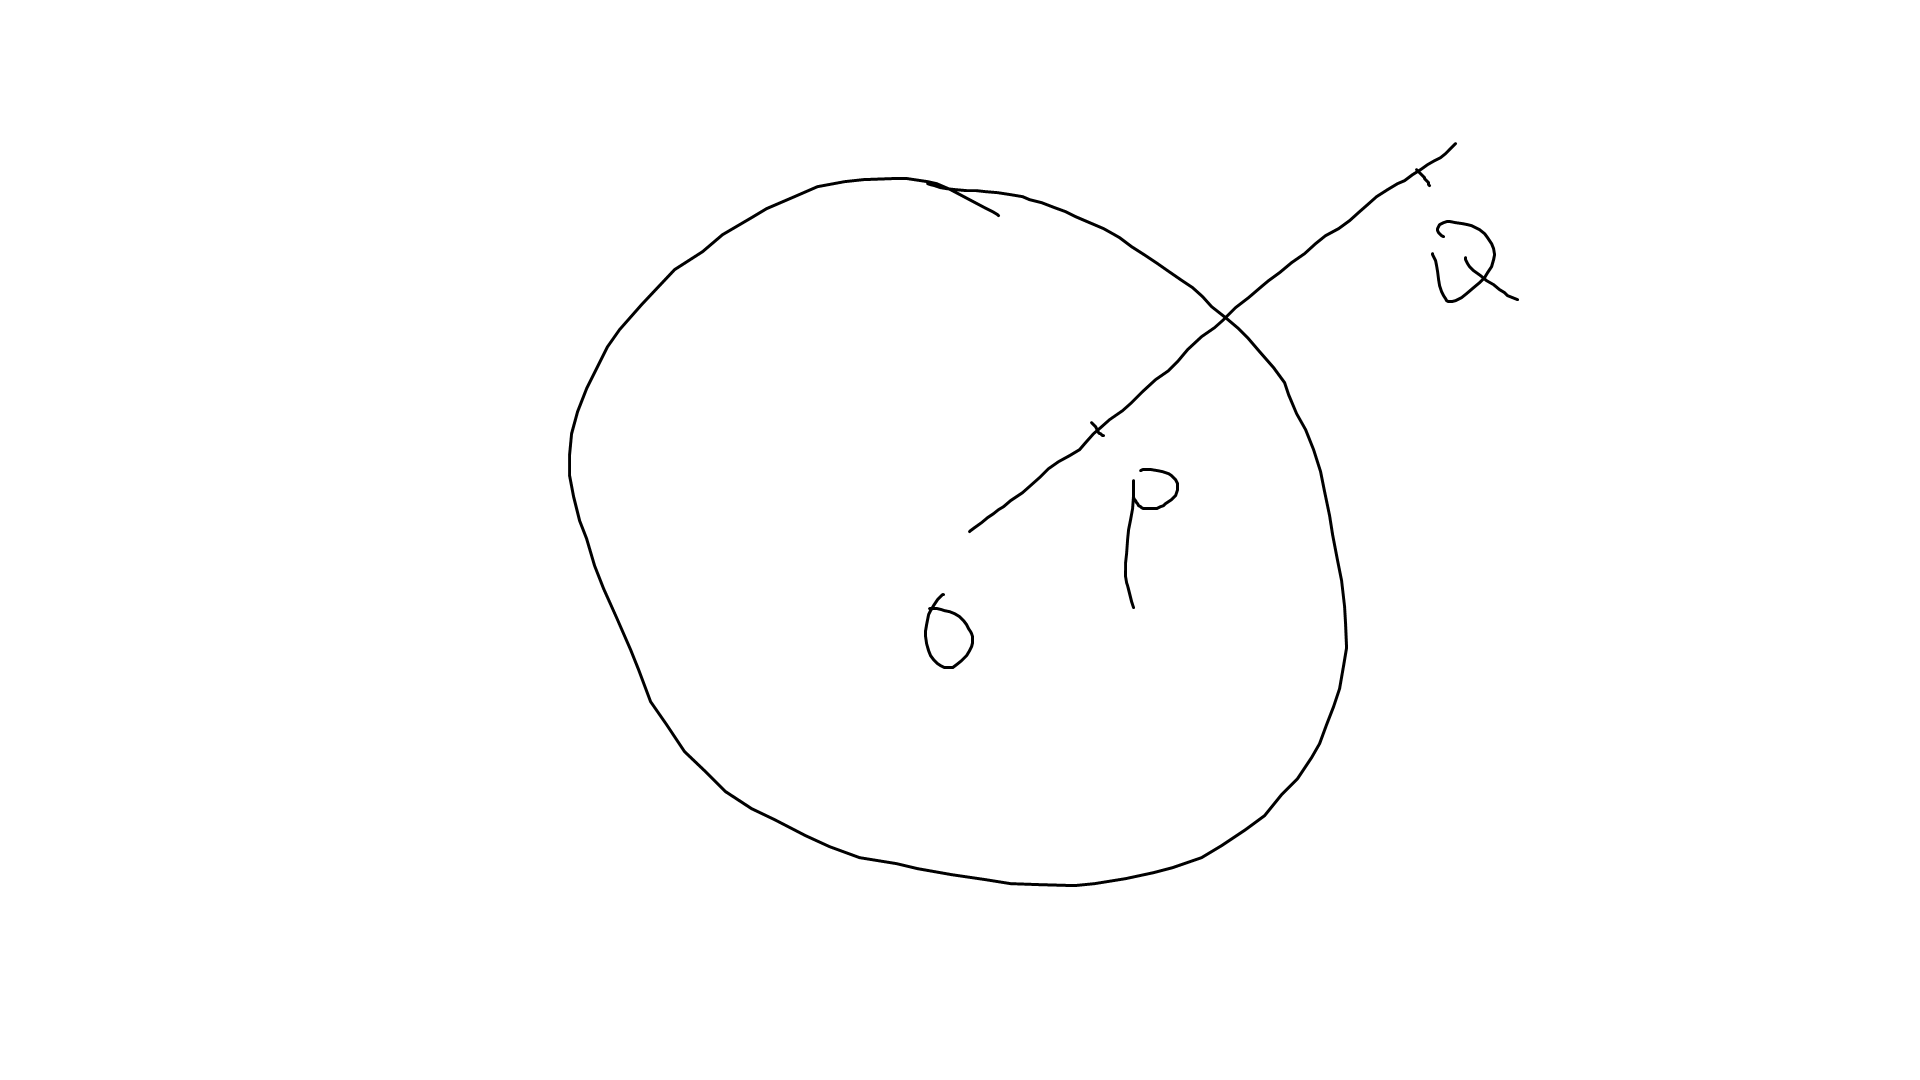
\includegraphics[scale=0.3]{Geometry_09}

If $P=(x,y,z) \in S^2$, $-P = (-x,-y,-z)$, then $\pi(P) = \frac{x+iy}{1-z}$, $\pi(-P) = \frac{-x-iy}{1+z}$. So
\begin{equation*}
\begin{aligned}
\pi(P) \cdot \overline{\pi(-P)} = \frac{-(x^2+y^2)}{1-z^2} = -1.
\end{aligned}
\end{equation*}
So $\pi(-P) = -\frac{1}{\zeta}$.

M$\ddot{o}$bius transformations act on $\C_\infty$ and form a group $G$ by composition. Any $A=\left(\begin{matrix}
a &b\\
c&d
\end{matrix}\right) \in GL(2,\C)$ defines a M$\ddot{o}$bius map
\begin{equation*}
\begin{aligned}
\zeta \to \frac{a\zeta + b}{c\zeta + d}.
\end{aligned}
\end{equation*}
For all $\lambda \in \C^* = \C \backslash\{0\}$, $\lambda A$ defines the same M$\ddot{o}$bius transformation.

Conversely, if $A_1$, $A_2$ give the same transformation, then $\exists \lambda \neq 0$ s.t. $A_1 = \lambda A_2$.

So $G \cong PGL(2,\C) = GL(2,\C)/\C^*$. i.e. $\C^* \cong \{\lambda I: \lambda \in \C^*\}$ is a normal subgroup.

It suffices to consider $\det A = 1$. If $\det \tilde{A} = 1$, $A = \lambda \tilde{A}$, then $1 = \det(\lambda \tilde{A}) = \lambda^2 \det A = \lambda^2$, i.e. $\lambda = \pm 1$.

So $G \cong PSL(2,\C) = SL(2,\C)/\pm I$ (group homomorphism $SL(2,\C) \to G$.

On $S^2$ we have rotations $SO(3)$ acting as isometries (see Q5 ES 1).

\begin{thm} 2.8\\
Via the stereographic projection $\pi$, every rotation of $S^2$ induces a M$\ddot{o}$bius map defined by a matrix in the subgroup $SU(2) \subset SL(2,\C)$ (the Special Unitary group of degree $n$ is the group of $n\times n$ orthogonal matrix with determinant 1). In the case $n=2$, we have
\begin{equation*}
\begin{aligned}
SU(2) = \left\{\left(\begin{matrix}
a & -b\\
\bar{b} & \bar{a}
\end{matrix}\right) : |a|^2+|b|^2 = 1\right\}
\end{aligned}
\end{equation*}
(Incidentally, $SU(2) \leftrightarrow S^3 \subset \R^4$).
\begin{proof}
(1) rotations $r(z,\theta)$ about the $z-$axis $\R(0,0,1)$ through angle $\theta$. The corresponding M$\ddot{o}$bius map is $\zeta \to e^{i\theta} \zeta$, i.e. a rotation of the complex plane, with matrix
\begin{equation*}
\begin{aligned}
\left(\begin{matrix}e^\frac{i\theta}{2} & 0\\
0 & e^{-\frac{i\theta}{2}} 
\end{matrix}\right)\in SU(2).
\end{aligned}
\end{equation*}

(2) rotation $r(y,\frac{\pi}{2})$ is
\begin{equation*}
\begin{aligned}
\left(\begin{matrix}
0 & 0 & 1\\
0 & 1 & 0\\
-1 & 0 & 0
\end{matrix}\right) \left(\begin{matrix}
x\\
y\\
z\\
\end{matrix}\right) = \left(\begin{matrix}
z\\
y\\
-x
\end{matrix}\right)
\end{aligned}
\end{equation*}
Which is rotation about $y-$axis through $\pm i$, sending $-1 \to \infty$, $1 \to 0$, $i \to i$. There is \emph{only one} such M$\ddot{o}$bius map
\begin{equation*}
\begin{aligned}
\zeta' = \frac{\zeta - 1}{\zeta + 1}
\end{aligned}
\end{equation*}
checking, this M$\ddot{o}$bius map gives $r(y,\frac{\pi}{2})$: $\zeta = \frac{x+iy}{1-z}$. So
\begin{equation*}
\begin{aligned}
\frac{\zeta-1}{\zeta+1} &= \frac{x+iy-1+z}{x+iy+1-z} = \frac{x-1+z+iy}{x+1-(z-iy)} = \frac{(z+iy)(x-1+z+iy)}{(x+1)(z+iy)+(x^2-1)}\\
&=\frac{(z+iy)(x-1+z+iy)}{(x+1)(z+iy+x-1)} = \frac{z+iy}{1+x} = \zeta'
\end{aligned}
\end{equation*}
$r(y,\frac{\pi}{2})$ corresponds to M$\ddot{o}$bius map with 
\begin{equation*}
\begin{aligned}
\frac{1}{\sqrt{2}} \left(\begin{matrix}
1 & -1\\
1 & 1
\end{matrix}\right) \in SU(2).
\end{aligned}
\end{equation*}

(3) $SO(3)$ is generated by $r(y,\frac{\pi}{2})$ and $r,(z,\theta)$ for $0\leq \theta < 2\pi$.

Observe $r(x,\varphi) = r(y,\frac{\pi}{2})r(z,\varphi)r(y,-\frac{\pi}{2})$ (we can see that by considering the image of $e_x$ under this map).

Also, $\forall\mathbf{v} \in S^2$ which is some unit vector, we can find $\varphi,\psi$ s.t. $g=r(z,\psi)r(x,\varphi):\mathbf{v} \to \left(\begin{matrix}
1\\0\\0
\end{matrix}\right)$.

$r(x,\varphi)$ rotates $\mathbf{v}
$ into the $(x,y)-$plane. Then for any given rotation we can write
\begin{equation*}
\begin{aligned}
r(\mathbf{v},\theta) = g^{-1} r(x,\theta) g
\end{aligned}
\end{equation*}

(4) Thus, via $\pi$, any rotation of $S^2$ correspond to a composition of M$\ddot{o}$bius maps of $\C_\infty$ with matrices in $SU(2)$.
\end{proof}
\end{thm}

This theorem gives a group homomorphism via $\pi$ of $SO(3)$ and $PSU(2) = SU(2) / \pm I$. This is injective. In fact it is also surjective, so this is an isomorphism.

\begin{thm} 2.9\\
The group $SO(3)$ of rotations of $S^2$ corresponds precisely with the subgroup $PSU(2) = SU(2) / \pm I$ of M$\ddot{o}$bius transformations acting on $\C_\infty$.
\begin{proof}
Let $g \in PSU(2) \subset G$. Then
\begin{equation*}
\begin{aligned}
g(z) = \frac{az-b}{\bar{b}z+\bar{a}}
\end{aligned}
\end{equation*}
Suppose first $g(0)=0$, so $b=0$, $a\bar{a} = 1$, $a=e^{\frac{i\theta}{2}}$ for some real $\theta$. Then $g$ corresponds to $r(z,\theta)$, i.e rotation about $z-$axis through $\theta$ (notation of the proof of Theorem 2.8).

In general, $g(0) = w \in \C_\infty$. Let $Q \in S^2$, $\pi(Q) = w$. Choose $A \in SO(3)$ with $A(Q) = \left(\begin{matrix}
0\\
0\\
-1
\end{matrix}\right)$. Let $\alpha \in PSU(2)$ the corresponding M$\ddot{o}$bius map (exists by Theorem 2.8). Then $\alpha(w)=0$, $\alpha \circ g$ fixes $0$. Hence $\alpha \circ g$ corresponds to $B = r(z,\tilde{\theta})$. Thus $g$ corresponds to $A^{-1}B$.
\end{proof}
\end{thm}

We've now shown that there is a $2-$to$-1$ map $SU(2) \to PSU(2) \cong SO(3)$ and a group homomorphism $SU(2) \cong S^3$.

\newpage

\section{Triangulations and the Euler number}
First, let's introduce one more 'geometry' - the \emph{locally Euclidean torus}.

\begin{defi}
The \emph{torus} $T$ is the set $\R^2/\Z^2$ of equivalence classes of $(x,y) \in \R^2$ with equivalence relation
\begin{equation*}
\begin{aligned}
(x_1,y_1) \sim (x_2,y_2) \iff \left\{\begin{array}{ll}
x_1-x_2 \in \Z\\
y_1-y_2 \in \Z
\end{array}\right.
\end{aligned}
\end{equation*}
Thus a point in $T$ represented by $(x,y)$ is a coset $(x,y)+\Z^2$ of the subgroup $\Z^2$ of the additive group $\R^2$.
\end{defi}

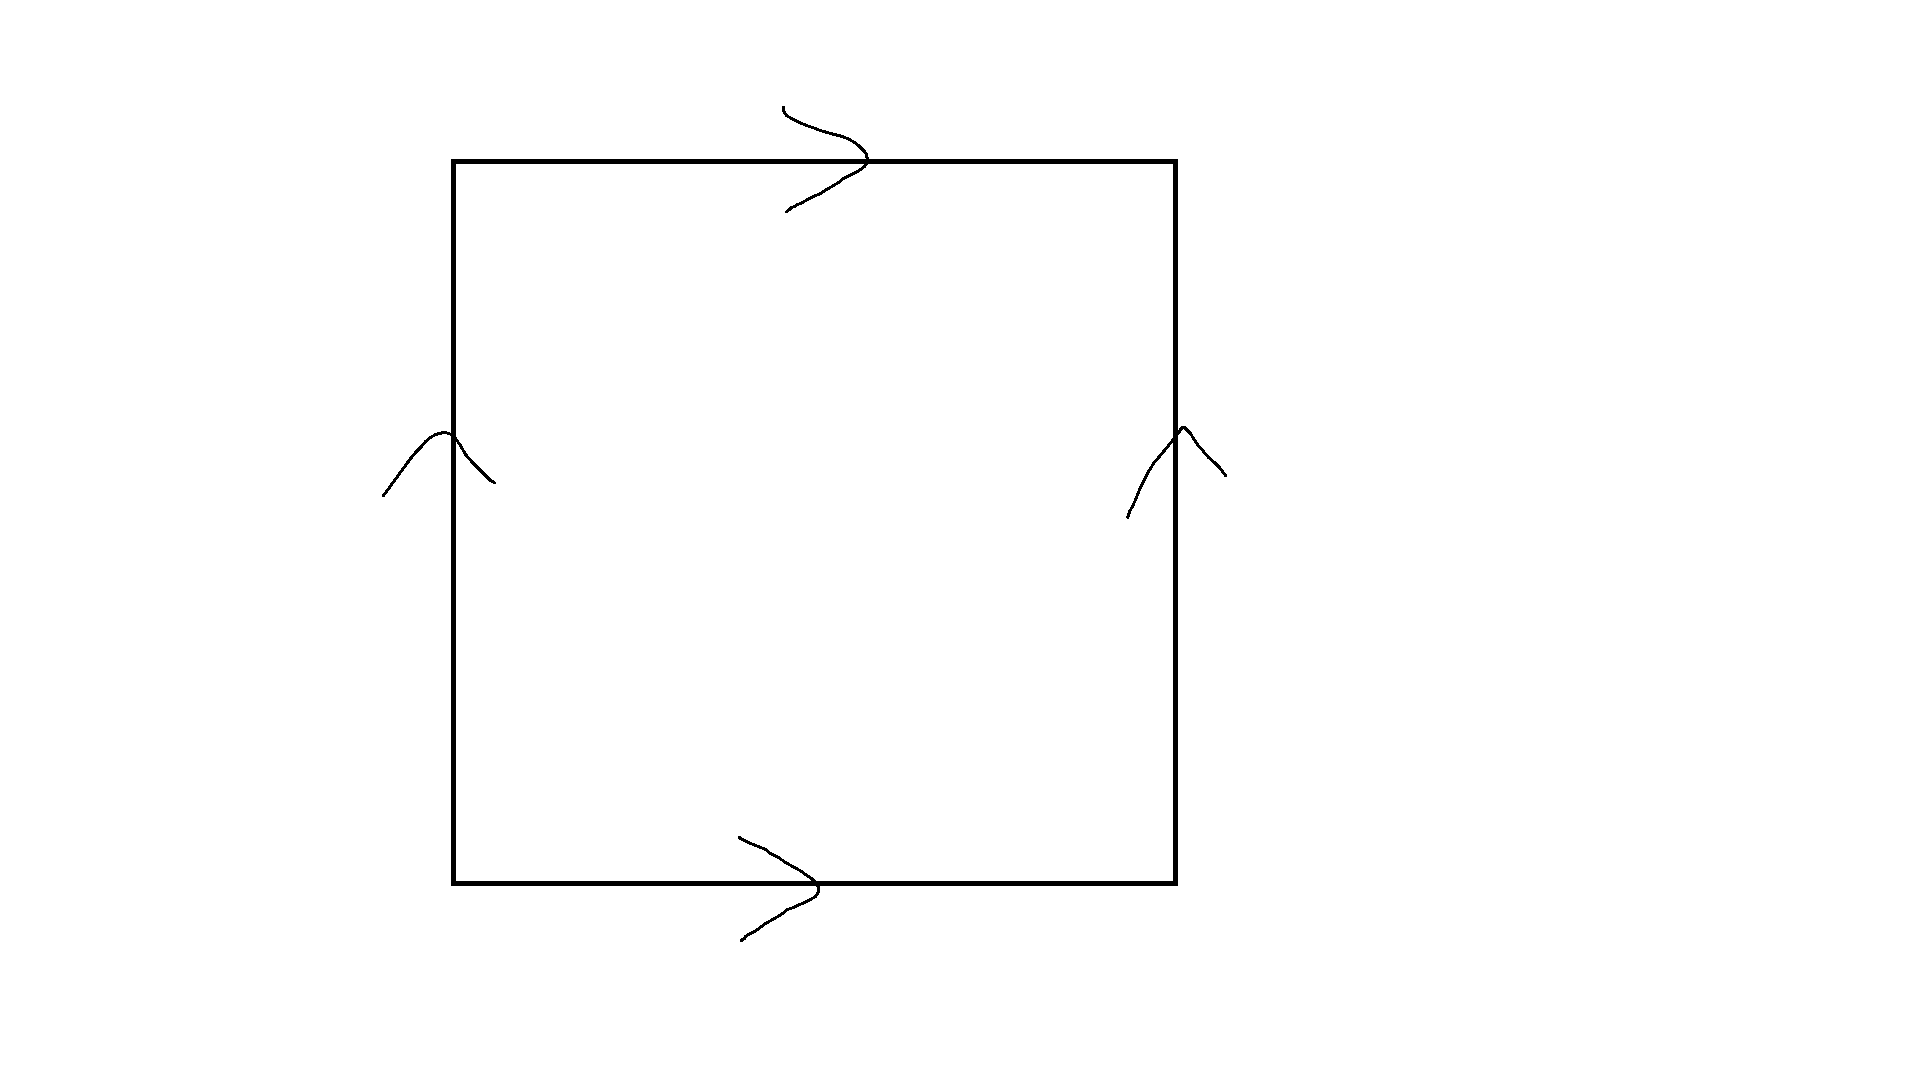
\includegraphics[scale=0.4]{Geometry_10}

For any closed square $Q \subset \R^2$ with side length $1$, define the \emph{distance} $d$, for $P_1,P_2 \in T$ to be
\begin{equation*}
\begin{aligned}
d(P_1,P_2) = \min \left\{|\mathbf{v}_1-\mathbf{v}_2| \mid \mathbf{v}_1,\mathbf{v}_2 \in \R^2, \mathbf{v}_i+\Z^2 = P_i \ \forall i\right\}.
\end{aligned}
\end{equation*}
It's easy to check that $(T,d)$ is a \emph{metric space}.

Let $Q^\circ$ denote the interior of $Q$. We have a natural map $f:Q^\circ \to T$ a natural bijection onto open $U \subset T$.

If $P \in Q^\circ$, then $f$ restricted to a small open disc about $P$ is an isometry. So $f:Q^\circ \to U$ is a homomorphism.

$d$ is said to be a \emph{locally Euclidean distance function} (for Euclidean metric).

\begin{rem}
$T$ may also be 'embedded' in $\R^3$.

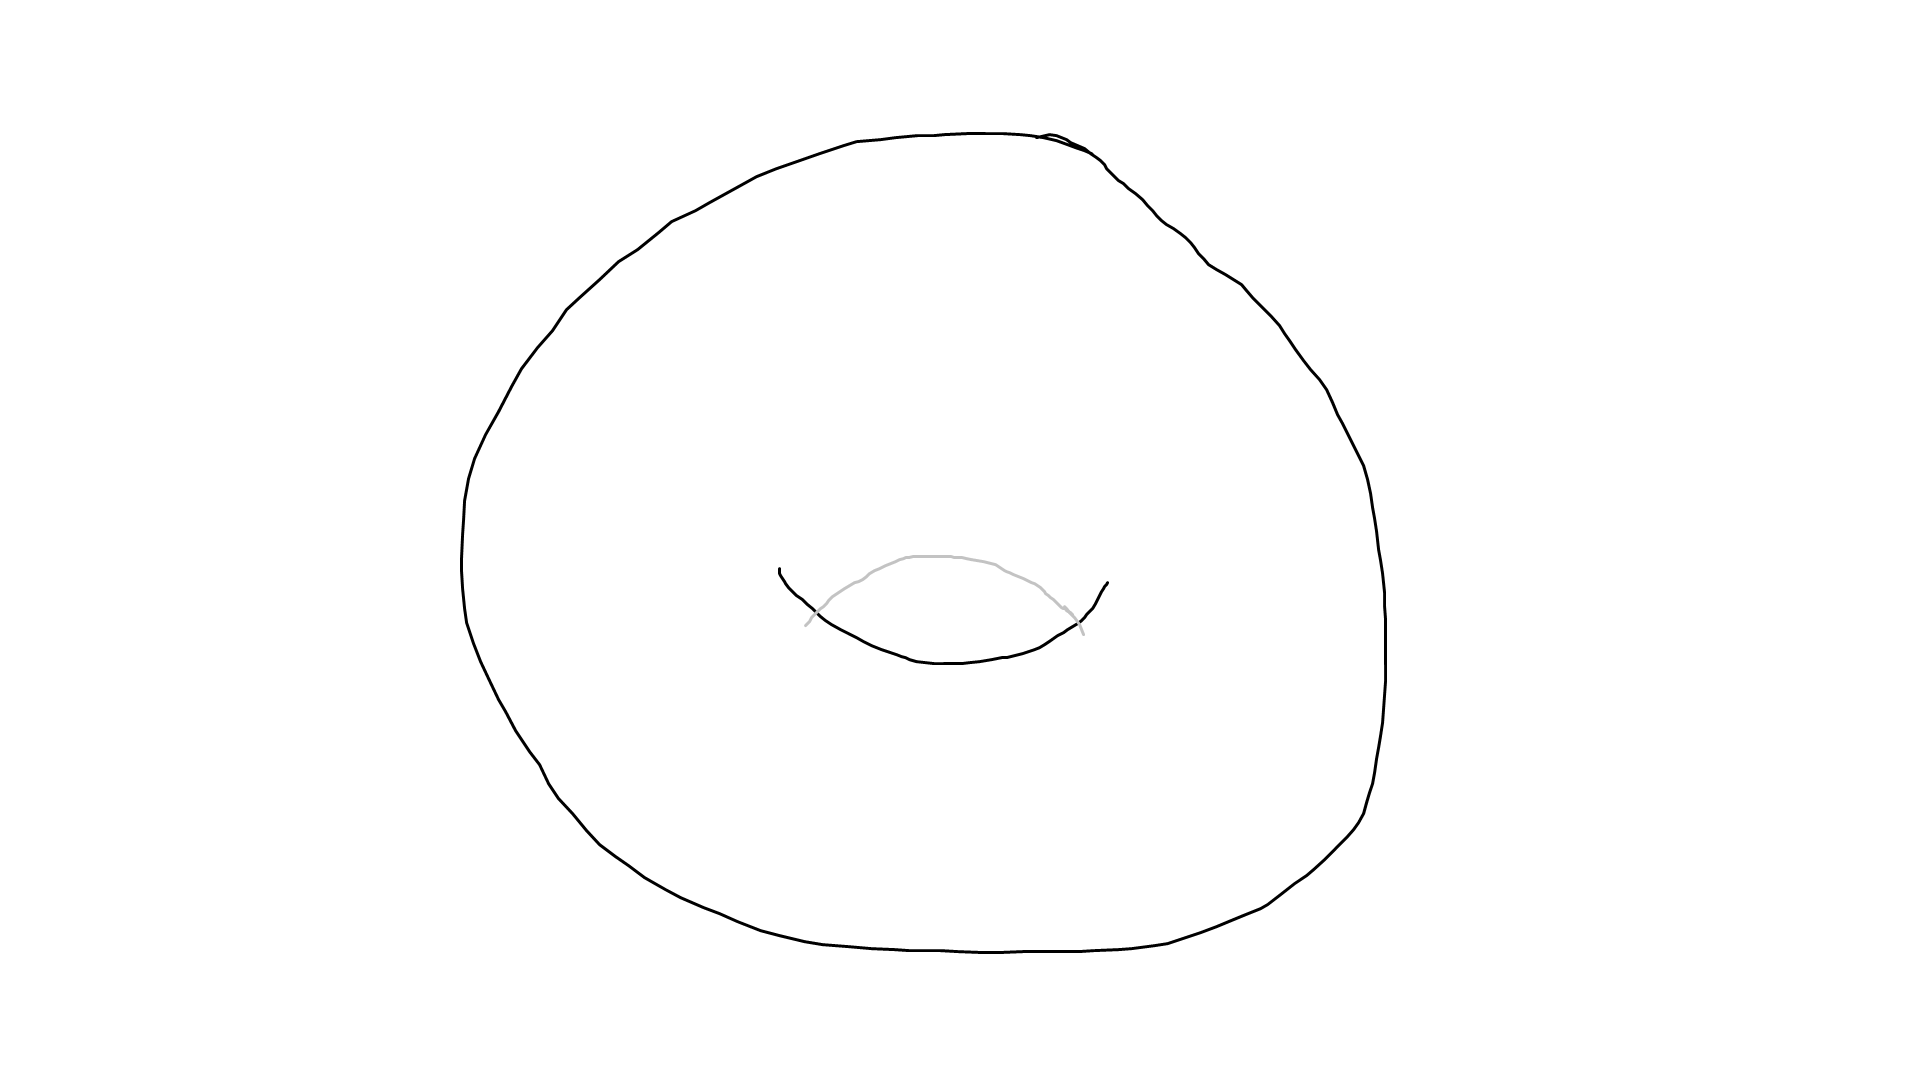
\includegraphics[scale=0.4]{Geometry_11}

The distance function we set by considering curves in $T \subset \R^3$ is \emph{not} the same.
\end{rem}

\begin{defi}
A \emph{topological triangle} on $X$ (here we usually consider $X$ being either $S^2$ or $T$) is the image $R \subset X$ of closed Euclidean triangle $\Delta \subset \R^2$ under a homomorphism $\Delta \to R$.
\end{defi}

\begin{eg}
A spherical triangle is a topological triangle (use a radial projection to a plane in $\R^3$ from $O$).
\end{eg}

\begin{defi}
A (topological) \emph{triangulation} $\tau$ of $X$ is a finite collection of topological triangles on $X$ s.t.\\
$\bullet$ $\forall$ two triangles are either disjoint or meet in exactly one edge or meet in exactly one vertex;\\
$\bullet$ each edge belongs to exactly two triangles.
\end{defi}

\begin{defi}
The \emph{Euler number} $e=e(X,\tau)$ is $e=F-E+V$ where $F$ is the number of triangles, $E$ is the number of edges, and $V$ is the number of vertices.

A fact from algebraic topology: $e$ is independent of the choice of $\tau$, so in fact $e=e(X)$.
\end{defi}

\begin{eg}
Consider $X=S^2$.

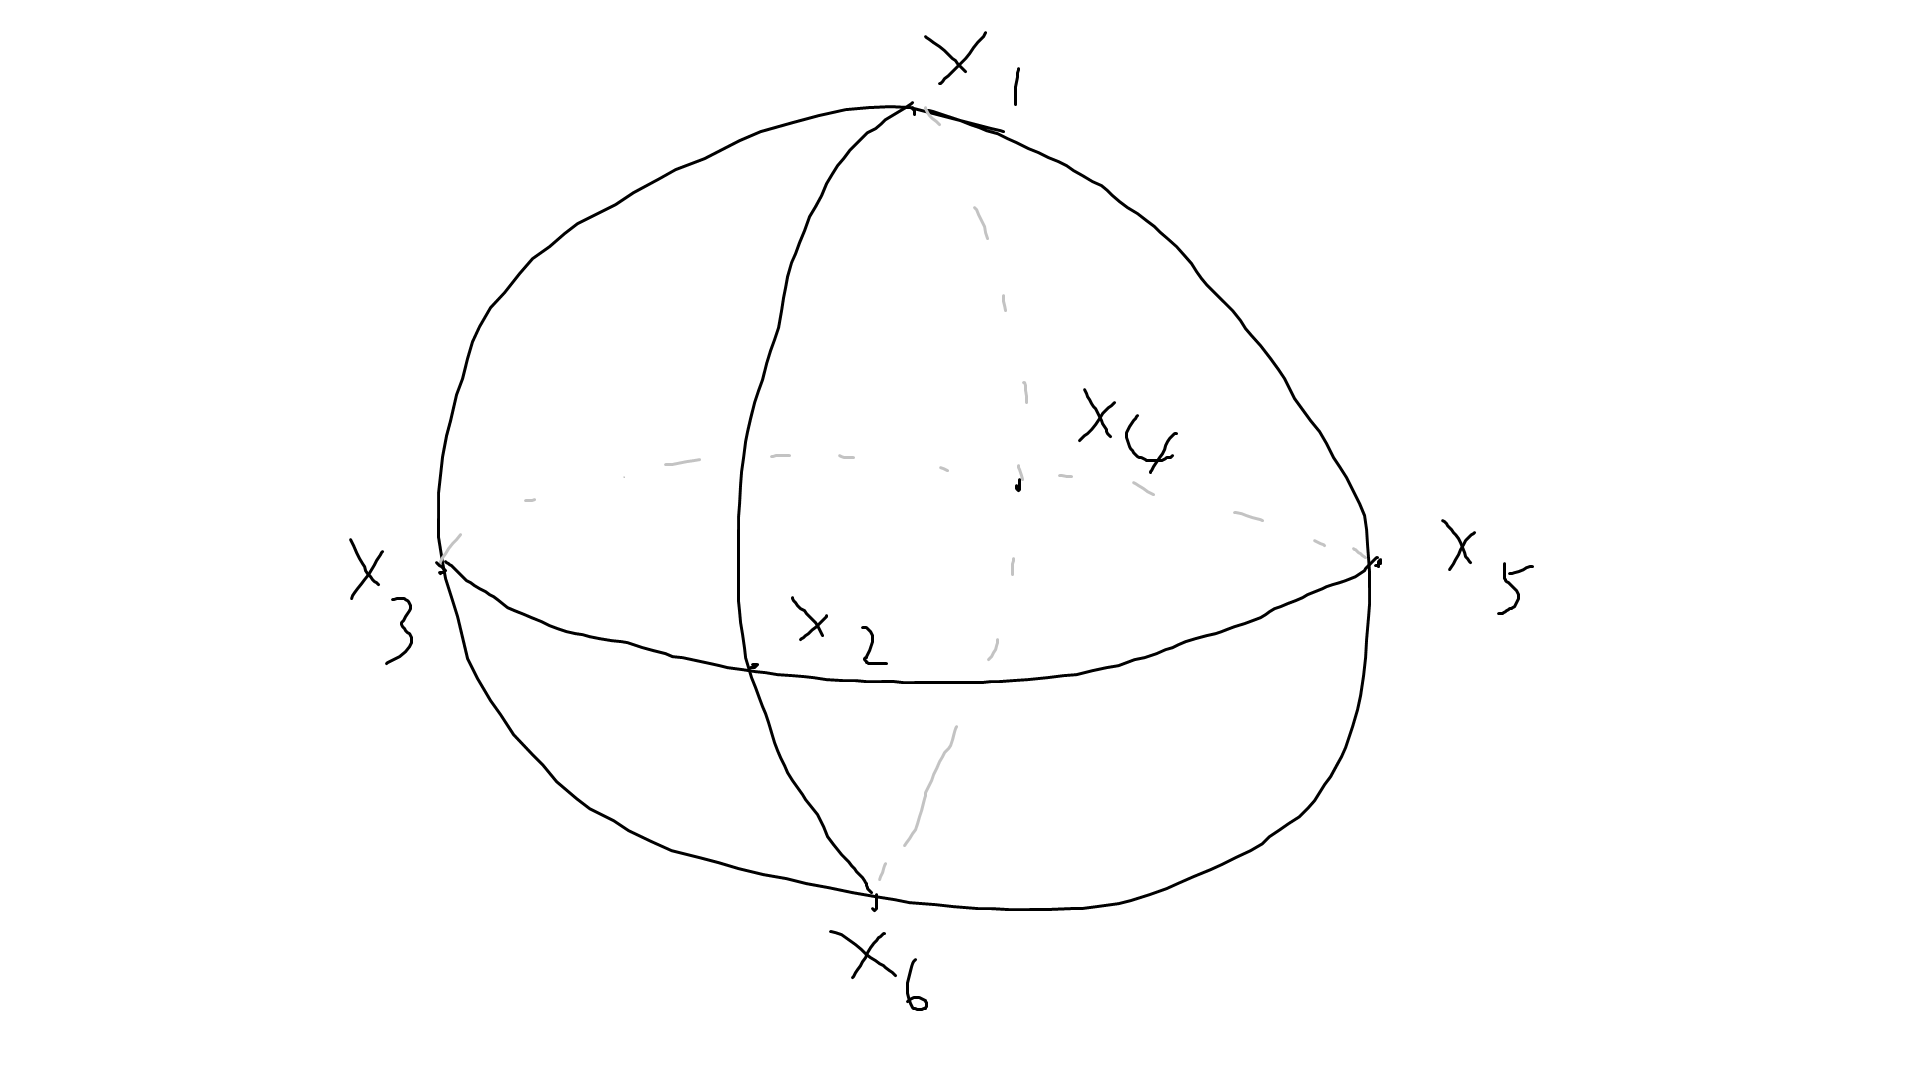
\includegraphics[scale=0.4]{Geometry_12}

We have $F=8$, $E=13$, $V=6$. So $e=2$.
\end{eg}

\begin{eg}
Consider $X=T$ (imagine the diagonals are straight lines).

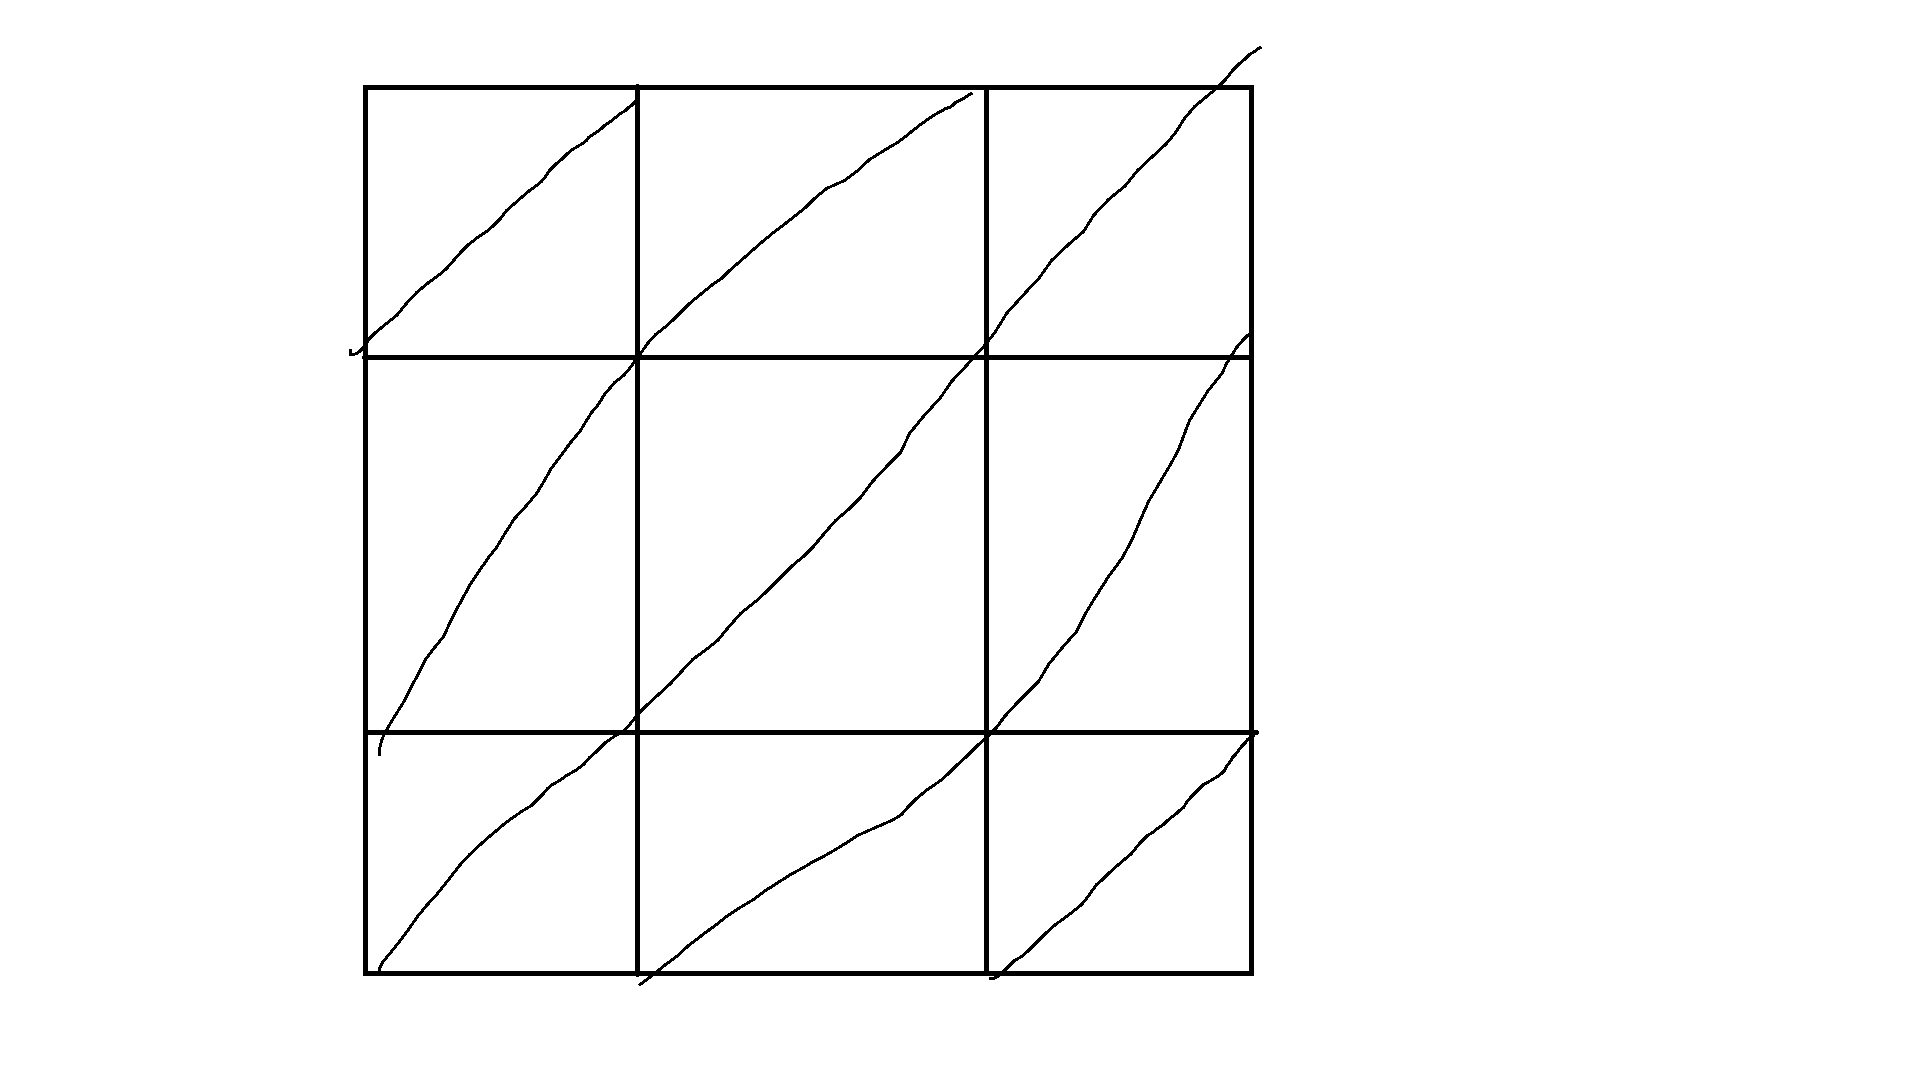
\includegraphics[scale=0.4]{Geometry_13}

We have $F=18$, $E=27$, $V=9$. So $e=0$.
\end{eg}

Note that in both cases we used \emph{geodesic triangles}, i.e. edges are spherical or Euclidean lines of $S^2$ or $T$ respectively.

\begin{rem} 
Take a look again at the definition of a \emph{triangulation}. We impose $X = \bigcup_{i=1}^F \Delta_i$ (can be deduced from other conditions -- exercise).
\end{rem}

\begin{prop} 3.1\\
For every geodesic triangles of $S^2$ or $T$, we have $e$ being $2$ or $0$ respectively.
\begin{proof}
Denote 'faces' of triangles $\Delta_1,...,\Delta_F$, and $\tau_i = \alpha_i + \beta_i + \gamma_i$, $i=1,...,F$, where $\alpha_i,\beta_i,\gamma_i$ are interior angles of the respective triangles. Then
\begin{equation*}
\begin{aligned}
\sum \tau_i = 2\pi V.
\end{aligned}
\end{equation*}
Also, $3F = 2E$ since every face has 3 edges and every edge is shared by 2 faces. So $F=2E-2F$.

In the case of $S^2$, by Gauss-Bonnet for $S^2$ (Proposition 2.6), area $\Delta_i = \tau_i - \pi$. So
\begin{equation*}
\begin{aligned}
4\pi &= \sum_{i=1}^F \Delta_i = \sum_{i=1}^F (\tau_i-\pi) = 2\pi V - \pi F\\
&= 2\pi V - 2\pi E + 2\pi F\\
&= 2\pi e
\end{aligned}
\end{equation*}
So $e=2$.

In the case of torus $T$, we have $\tau_i = \pi$ $\forall i$ as $T$ is locally Euclidean. So
\begin{equation*}
\begin{aligned}
2\pi V = \sum_{i=1}^F \tau_i = \pi F
\end{aligned}
\end{equation*}
So $2V=F = 2E-2F$. So $V-E+F=0$.
\end{proof}
\end{prop}

\begin{rem}
We may use topological polygonal decomposition (rather than topological triangles), and proposition 3.1 will still hold. Then considering $S^2$, obtain Euler's formula
\begin{equation*}
\begin{aligned}
V-E+F=2.
\end{aligned}
\end{equation*}
\end{rem}

\newpage

\section{Hyperbolic Geometry}

$\bullet$ Revision of derivatives and the chain rule: let $U \subset \R^n$ be open, $f=(f_1,...,f_n): U \to \R^m$ is smooth ($C^\infty$) if each $f_i$ has continuous partial derivatives of every order. This certainly implies differentiability (1st order partial derivatives are continuous).

The derivative of $f$ at $a \in U$ is a linear map $df_u:\R^n \to \R^m$ (i.e. $DF|_a$ in Analysis II), so that
\begin{equation*}
\begin{aligned}
\frac{||f(a+h)-f(a)-df_a \cdot h||}{||h||} \to 0
\end{aligned}
\end{equation*}
as $h \to 0$ in $\R^n$.

If $m=1$, then $df_n$ is expressed as $\left(\frac{\partial f}{\partial x_1}(a),...,\frac{\partial f}{\partial x_i}(a)\right)$ via
\begin{equation*}
\begin{aligned}
(h_1,...,h_n) \to \sum_{i=1}^n \frac{\partial f}{\partial x_i}(a) h_i
\end{aligned}
\end{equation*}

For general $m$, we may use the \emph{Jacobi matrix}
\begin{equation*}
\begin{aligned}
J(f)_a = \left(\frac{\partial f_i}{\partial x_j}(a)\right)
\end{aligned}
\end{equation*}
and $\mathbf{h} \to J(f)_a \mathbf{h}$.

\begin{eg}
Holomorphic (analytic) functions of complex variable $f:U \subset \C \to \C$. $f'(z)$ is defined by
\begin{equation*}
\begin{aligned}
\frac{|f(z+w)-f(z)-f'(z)w|}{|w|} \to 0
\end{aligned}
\end{equation*}
as $w \to 0$. Let $f'(z) = a+ib$, $w=h_1+ih_2$. Then
\begin{equation*}
\begin{aligned}
f'(z)w = (ah_1-bh_2)+i(ah_2+bh_1)
\end{aligned}
\end{equation*}
now $R^2 \cong \C$, $f: U \subset \R^2 \to \R^2$ then $df_z: \R^2 \to \R^2$ is given by
\begin{equation*}
\begin{aligned}
\left(\begin{matrix}
a & -b\\
b & a
\end{matrix}\right)
\end{aligned}
\end{equation*}
\end{eg}

Let $U \subset \R^n$, $v \subset \R^p$ be open, $f:U \to \R^m$, $g: V \to U$ be smooth functions. Then
\begin{equation*}
\begin{aligned}
f \circ g : V \to \R
\end{aligned}
\end{equation*}
has derivative
\begin{equation*}
\begin{aligned}
d(f\circ g)_p = (df)_{g(p)} \circ (dg)_p
\end{aligned}
\end{equation*}
for $p \in V$. Or, using the Jacobi matrices,
\begin{equation*}
\begin{aligned}
J(f \circ g)_p = J(f)_{g(p)} J(g)_p
\end{aligned}
\end{equation*}
by matrix multiplication.

\subsection{Riemannian metrics (on open sets of $\R^2$)}
We use coordinates $(u,v) \in \R^2$, let $V \subset \R^2$ be open. A Riemannian matrix is defined by giving $C^\infty$ functions $E,F,G: V \to \R$ s.t. 
\begin{equation*}
\begin{aligned}
\left(\begin{matrix}
E(p) & F(p)\\
F(p) & G(p)
\end{matrix}\right)
\end{aligned}
\end{equation*}
is a positive-definite matrix for every $p \in V$.

Thus $\forall p \in V$, the $2 \times 2$ matrix defines an inner product in $\R^2$(c.f. Linear Algebra), i.e.
\begin{equation*}
\begin{aligned}
\left<e_1,e_1\right>_p = E(p),\\
\left<e_2,e_2\right>_p = G(p),\\
\left<e_1,e_2\right>_p = F(p).
\end{aligned}
\end{equation*}
e.g. $E=G=1$, $F=0$ gives the standard Euclidean inner product.

\begin{notation}
We introduce the notation $Edu^2 + 2Fdudv + Gdv^2$, where $u:V \to \R$, $v:V \to \R$ the coordinates are $C^\infty$ functions.

$du_p, dv_p:\R^2 \to \R$ have derivatives $(h_1,h_2) \to h_1 , (h_1,h_2) \to h_2$.

Thus $du = du_p$, $dv = dv_p$ are elements of the dual space $(\R^2)^*$. Moreover they are LI. So they form a basis of $(\R^2)^*$, which is the dual basis to the standard basis of $\R^2$.

Thus $du^2,dudv,dv^2$ are bilinear forms on $\R^2$, with
\begin{equation*}
\begin{aligned}
du^2 (h,k) = du(h)du(k),\\
dudv(h,k)=\frac{1}{2}(du(h)dv(k)+du(k)dv(h),\\
dv^2(h,k) = dv(h)dv(k)
\end{aligned}
\end{equation*}
corresponding to the matrices
\begin{equation*}
\begin{aligned}
\left(\begin{matrix}
1 & 0\\
0 & 0
\end{matrix}\right),
\left(\begin{matrix}
0 & 1/2\\
1/2 & 0
\end{matrix}\right),
\left(\begin{matrix}
0 & 0\\
0 & 1
\end{matrix}\right)
\end{aligned}
\end{equation*}
\end{notation}
and so
\begin{equation*}
\begin{aligned}
Edu^2 + 2Fdudv+Gdv^2
\end{aligned}
\end{equation*}
is of the form
\begin{equation*}
\begin{aligned}
\left(\begin{matrix}
E & F\\
F & G
\end{matrix}\right).
\end{aligned}
\end{equation*}

\begin{defi}
The \emph{length} of a smooth curve $\gamma = (\gamma_1(t),\gamma_2(t)) : [0,1] \to V \subset \R^2$ is
\begin{equation*}
\begin{aligned}
\int_0^1 \left(E\dot{\gamma}_1^2 + 2F\dot{\gamma}_1\dot{\gamma}_2 + G\dot{\gamma}_2^2\right)^{1/2} dt
\end{aligned}
\end{equation*}
where the dot represents derivatievs with respect to $t$. Note that the integrand is just $\left<\dot{\gamma}(t),\dot{\gamma}(t)\right>_{\gamma(t)}$ (c.f. proposition 1.2).

The \emph{area} of a region $W \subset V$ is defined as
\begin{equation*}
\begin{aligned}
\int_W (EG-F^2)^{1/2} dudv
\end{aligned}
\end{equation*}
which is the Gram determinant.
\end{defi}

\begin{eg}
Consider $V = \R^2$ with Riemmanian metric
\begin{equation*}
\begin{aligned}
\frac{4(du^2+dv^2)}{(1+u^2+v^2)^2}
\end{aligned}
\end{equation*}
we shall see that via stereographic projection, $\pi:S^2 \setminus \{N\} \to \R_{u,v}^2$.
\end{eg}

Recap on the Riemannian metrics. Suppose we have an open $V \subset \R^2$. We may think of $\R^2$ as an affine space $A^2$, or a vector space $\R^2$. It's easy to have identification $A^2 \cong \R^2$ (need to choose where to map the $\mathbf{0} \in \R^2$). We can attach a copy of $\R^2$ at $P \in A^2$.

Now $P \in S^2 \setminus \{N\}$, $P \neq N$. The tangent plane to $S^2$ at $P$ is
\begin{equation*}
\begin{aligned}
\{ \mathbf{x} \in \R^3: \mathbf{x} \cdot \overrightarrow{OP} = 0\}
\end{aligned}
\end{equation*}
$\mathbf{x} = \overrightarrow{OX} - \overrightarrow{OP}$. Consider $\pi(P) = (u,v) \in \R^2$ where $\pi$ is the stereographic projection.

\begin{eg} (see sheet 3)\\
For all $x_1, x_2 \perp \overrightarrow{OP}$, $\mathbf{x}_1 \cdot \mathbf{x}_2 = \left<d\pi|_P(\mathbf{x}_1),d\pi |_P(\mathbf{x}_2)\right>_{\pi(P)}$.

This formula defines an inner product $\left<\cdot,\cdot\right>_{\pi(P)}$ on a 'copy of $\R^2$' at $\pi(P)$. Thus we induced an instance of Riemannian metric on $V=\R^2$ using $d\pi_P$ for $P \in S^2 \setminus \{N\}$.
\end{eg}

\begin{defi}
Let $V,\tilde{V} \subset \R^2$ be open and endowed with Riemannian metrics. Denote $\left<\cdot,\cdot\right>_P$, $O \in V$ and $\left<\cdot,\cdot\right>^{\sim}_Q$, $Q \in \tilde{V}$ the respective inner products.

A \emph{diffeomorphism} $\varphi:V \to \tilde{V}$ is called an \emph{isometry} iff for all $P \in V$, $Q = \varphi(p)$ we have
\begin{equation*}
\begin{aligned}
\left<\mathbf{x},\mathbf{y}\right>_P = \left<d\varphi_P(\mathbf{x}),d\varphi_P(\mathbf{y})\right>^\sim_{\varphi(P) =Q}
\end{aligned}
\end{equation*}
for all $\mathbf{x},\mathbf{y} \in \R^2$.
\end{defi}

If $\gamma:[0,1]\to V$ be a $C^1$ curve, then $\tilde{\gamma} = \varphi \circ \gamma: [0,1] \to \tilde{V}$ is also a $C^1$ curve. Let $P=\gamma(t)$, so $\varphi(P) = \tilde{\gamma}(t)$. We have
\begin{equation*}
\begin{aligned}
\left<\tilde{\gamma}'(t),\tilde{\gamma}'(t)\right>_{\tilde{\gamma}(t)} = \left<d\varphi_P (\gamma'(t)),d\varphi_P (\gamma'(t))\right>_{\varphi(P)}
\end{aligned}
\end{equation*}
by chain rule. If $\varphi$ is an isometry then the above is equal to
\begin{equation*}
\begin{aligned}
\left<\gamma'(t),\gamma'(t)\right>_{\gamma(t)}
\end{aligned}
\end{equation*}
Then (by integrating)
\begin{equation*}
\begin{aligned}
length(\tilde{\gamma}) = length(\gamma) = \int_0^1 \left<\gamma'(t),\gamma'(t)\right>^{1/2}_{\gamma(t)} dt.
\end{aligned}
\end{equation*}
So isometries preserve lengths of curves, and so distances.

\subsection{Two models for the hyperbolic plane}
\begin{defi}
The \emph{Poincare's disc model} for the hyperbolic plane is given by $D \subset \C \cong \R^2$, $D = \{|\zeta|<1\}$ and a Riemannian metric
\begin{equation*}\tag{*}
\begin{aligned}
\frac{4(du^2+dv^2)}{(1-u^2-v^2)^2} = \frac{4|d\zeta|^2}{(1-|\zeta|^2)^2}
\end{aligned}
\end{equation*}
where $\zeta = u+iv$, $d\zeta = du+idv$ (e.g. $d\zeta:\C \to \C$ linear map). Thus element of the dual complex vector space(??). $|d\zeta|^2 = du^2 + dv^2$.
\end{defi}

(*) is a scaling of the Euclidean metric $du^2+dv^2$ by a factor depending on the polar radius $r=|\zeta|$: distances are scaled by $\frac{2}{1-r^2}$ and areas by $\frac{4}{(1-r^2)^2} = \sqrt{EG-F^2}$.

The upper half plane is $H = \{z \in \C: \Im(z) > 0\}$. $D$ bijects to $H$ via M$\ddot{o}$bius transformation $\zeta \in D \to \frac{i(1+\zeta)}{1-\zeta} \in H$.

We fix notation $z \in H$, $z=x+iy$, $z = \frac{1(i+\zeta)}{1-\zeta}$, $\zeta \in D$, $\zeta = u+iv$, $\zeta = \frac{z-i}{z+i}$.

We shall prove this induces a Riemann metric on $H$, so that $\zeta \to z$ as the above M$\ddot{o}$bius map is an isometry $D \to H$.

The Euclidean product on $\C(\cong \R^2)$ is $\left<w_1,w_2\right> = \Re(w_1\bar{w}_2) = \frac{w_1\bar{2}_2+\bar{w}_1w_2}{2}$.

So if $\left<\cdot,\cdot\right>$ is Euclidean at $\zeta$, then at $z$ s.t. $\zeta = \frac{z-i}{z+i}$ we require
\begin{equation*}
\begin{aligned}
\left<w_1,w_2\right>_z = \left<\frac{d\zeta}{dz}w_1,\frac{d\zeta}{dz} w_2\right>_{Eud} = \left|\frac{d\zeta}{dz}\right|^2 \Re(w_1\bar{w}_2)
\end{aligned}
\end{equation*}
i.e. on $H$, we obtain a Riemannian metric
\begin{equation*}
\begin{aligned}
\left|\frac{d\zeta}{dz}\right|^2 (dx^2+dy^2) = |dz^2|
\end{aligned}
\end{equation*}
We compute
\begin{equation*}
\begin{aligned}
\frac{d\zeta}{dz} = \frac{1}{z+i} - \frac{z-i}{(z+i)^2} = \frac{2i}{(z+i)^2},
\end{aligned}
\end{equation*}
\begin{equation*}
\begin{aligned}
1-|\zeta|^2 = 1-\frac{|z-i|^2}{|z+i|^2}
\end{aligned}
\end{equation*}
so
\begin{equation*}
\begin{aligned}
\frac{1}{1-|\zeta|^2} = \frac{|z+i|^2}{|z+i|^2-|z-i|^2} = \frac{|z+i|^2}{4\Im z}
\end{aligned}
\end{equation*}
Putting everything together, the metric on $H$ corresponding $\frac{4|d\zeta|^2}{(1-|\zeta|^2)^2}$ is
\begin{equation*}
\begin{aligned}
4 \cdot \frac{4}{|z+i|^4} \cdot \left(\frac{|z+i^2}{4\Im z}\right)^2 \cdot |dz|^2 = \frac{|dz|^2}{(\Im z)^2} = \frac{dx^2 + dy^2}{y}
\end{aligned}
\end{equation*}
Note that on $H$ we got a scaling of Euclidean matric: distances scaled by $1/y$ and areas scaled by $1/y^2$.

\begin{defi}
The \emph{upper half-plane} model for the hyperbolic plane is $H$ with metric
\begin{equation*}
\begin{aligned}
\frac{dx^2+dy^2}{y^2}
\end{aligned}
\end{equation*}
\end{defi}
Consider $PSL(2,\R) = \left\{z \to \frac{az+b}{cz+d}:a,b,c,d \in \R,ad-bc = 1\right\}$, the subgroup of M$\ddot{o}$bius transformations sending $\R \cup \{\infty\} \to \R \cup \{\infty\}$ and $H \to H$.

\begin{prop} 4.1\\
The elements of $PSL(2,\R)$ are \emph{isometries} of $H$ and thus preserve lengths of curves.
\begin{proof}
Easy to check that $PSL(2,\R)$ is generated by:\\
$z \to z+a$, $a \in \R$;\\
$z \to az$, $a\in R^+$;\\
$z \to -1/z$.

It suffices to show that every of these three maps preserves the Riemannian metric
\begin{equation*}
\begin{aligned}
\frac{|dz|^2}{(\Im z)^2} = \frac{dx^2+dy^2}{y^2}
\end{aligned}
\end{equation*}
\end{proof}
\end{prop}

The first two are clear. We check the third one $f(z) = -1/z$:\\
$w \to f'(z)w$, $f'(z) = 1/z^2$, so
\begin{equation*}
\begin{aligned}
d\left(\frac{-1}{z}\right) = \frac{dz}{z^2},\\
\left|d\left(\frac{-1}{z}\right)\right|^2 = \frac{|dz|^2}{|z|^4},\\
\Im \left(\frac{-1}{z}\right) = \frac{-1}{|z|^2} \Im \bar{z} = \frac{\Im z}{|z|^2}
\end{aligned}
\end{equation*}
Thus
\begin{equation*}
\begin{aligned}
\frac{|d(-1/z)|^2}{|\Im (-1/z)|^2} = \frac{1/|z|^4 |dz|^2}{(\Im z)^2 / |z|^4} = \frac{|dz|^2}{(\Im z)^2}
\end{aligned}
\end{equation*}

\begin{rem}
Each $z \to az+b$ for $a,b \in \R$, $a>0$ in $PSL(2,\R)$ Hence $PSL(2,\R)$ acts \emph{transitively} on $H$.
\end{rem}
Each M$\ddot{o}$bius transformation preserves the set of circles and straight lines in $\C$. If $L=i\R$, $g \in PSL(2,\R)$, then $g(L)$ is either a circle centred at a point in $\R$ or straight line perpendicular to $\R$.

Put $L^+ = \{it:t>0\}$. Then $g(L^+)$ is either a semicircle with ends in $\R$ or vertical half line starting at a point in $\R$. We call these lines the hyperbolic lines in $H$.

\begin{lemma} 4.2\\
Through any two points $z_1,z_2 \in H$, there is a unique hyperbolic line $l$.
\begin{proof}
This is clear when $\Re z_1 = \Re z_2$. If not, then the perpendicular bisector of $z_1z_2$ intersect $\R$ at one point, which is the centre of the semicircle.

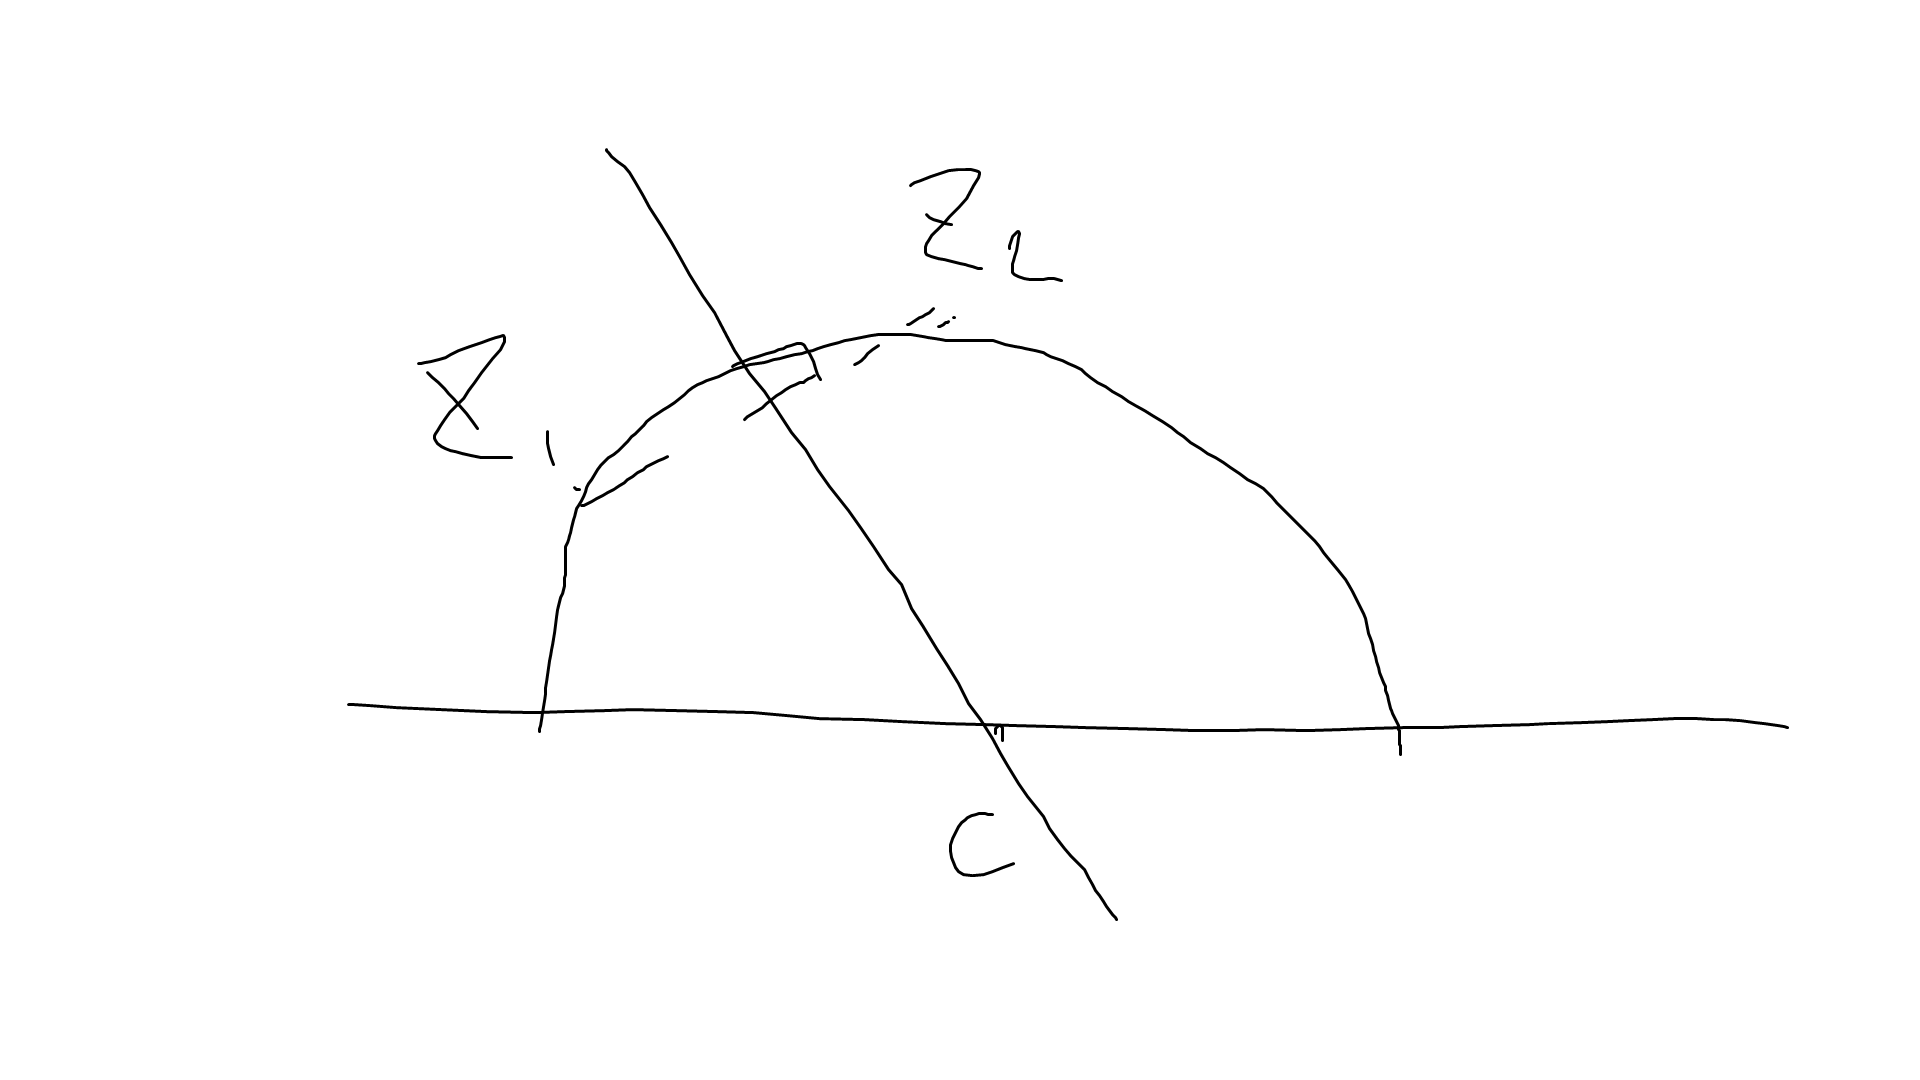
\includegraphics[scale=0.4]{Geometry_14}
\end{proof}
\end{lemma}

\begin{lemma} 4.3\\
$PSL(2,\R)$ acts \emph{transitively} on the set of hyperbolic lines.
\begin{proof}
It suffices to show that for all hyperbolic lines $l$, there exists $g \in PSL(2,\R)$ s.t. $g(l)=L^+$. This is clear when $l$ is a vertical half line. If $l$ is a semicircle, endpoints $s<t\in \R$, then $g(z) = \frac{z-t}{z-s}$ which is valid as the determinant of the corresponding matrix is positive. Also, $g(t) = 0$, $g(s) = \infty$, and the only half line through them is $L^+$.
\end{proof}
\end{lemma}

\begin{rem}
Furthermore, we can achieve $g(s)=0$, $g(t) = \infty$ by composing with $z \to -1/z$. Also we can map all given point $P \in l$ to $g(P) = i \in L^+$ (compose with $z \to az$, $a>0$).
\end{rem}

\begin{defi}
Given two points $z_1,z_2 \in H$, the \emph{hyperbolic distance}, $\rho(z_1,z_2)$, is the length of segment $[z_1,z_2] \subset l$ of the unique hyperbolic line through $z_1,z_2$. Then $PSL(2,\R)$ preserves $\rho$ (by Lemma 4.2, Proposition 4.1 and some previous theory).
\end{defi}

\begin{prop} 4.4\\
If $\gamma:[0,1] \to H$ is piece-wise $C^1$-norm with $\gamma(0) =z_1,$, $\gamma(1) = z_2$, then $length(\gamma) \geq \rho(z_1,z_2)$ with equality holds iff $\gamma$ is the hyperbolic line through $z_1$ and $z_2$ parameterized monotonically (i.e. no going back).
\begin{proof}
We assume $\gamma$ is $C^1$. $\exists$ $g \in PSL(2,\R)$ that takes $g(l) to L^+$ (which is an isometry). So WLOG let $z_1 = iu$, $z_2 = iv$, $u<v \in \R$. Then write $\gamma(t) = x(t) + iy(t)$, we have
\begin{equation*}
\begin{aligned}
length(\gamma) &= \int_0^1 \frac{1}{y} \sqrt{\dot{x}^2 + \dot{y}^2} dt\\
&\geq \int_0^1  \frac{|\dot{y}|}{y}dt\\
&\geq \left|\int_0^1 \frac{\dot{y}}{y} dt\right|\\
&\geq \log y(t) |_0^1
\end{aligned}
\end{equation*}
Thus
\begin{equation*}
\begin{aligned}
\rho(z_1,z_2) = \log \frac{v}{u}
\end{aligned}
\end{equation*}
Equality holds only if $\dot{x} \equiv 0$, $\dot{y} \geq 0$, i.e. monotonic.
\end{proof}
\end{prop}

\begin{rem}
This proposition implies triangle inequality for $\rho(\cdot,\cdot)$: $length(\gamma) = \rho(z_1,z_2) \leq \rho(z_1,z_3) + \rho(z_3,z_2)$, with equality iff $z_3 \in \gamma$.

Thus $(H,\rho)$ is a metric space.
\end{rem}

Now consider the Geometry of the disc model.

Recall $\zeta \in D \to z = \frac{1+\zeta}{1-\zeta} \in H$.\\
$z \in H \to \zeta = \frac{z-i}{z+i}\in D$.

So (i) $PSL(2,\R) \cong$ the group of M$\ddot{o}$bius transformations sending $|\zeta| = 1$ to itself and $D \to D$. Call this group $G$.\\
(ii) Hyperbolic lines in $D$ are segments of circles meeting  $|\zeta| = 1$ orthogonally including diameters.\\
(iii) $G$ acts transitively on hyperbolic lines in $D$.\\
(iv) The length minimizing curves are segments of hyperbolic lines parameterized monotonically.

Let $\rho$ denote the hyperbolic distance.

\begin{lemma} 4.5\\
(i) Rotations $z \to e^{i\theta} z$ ($\theta \in \R$) are in $G$;\\
(ii) if $a \in D$, then $g(z) = \frac{z-a}{1-\bar{a}z}$ is in $G$.
\begin{proof}
It's easy to see as these are linear maps, $|e^{i\theta} z| = |z|$, $d(e^{i\theta} z)| = dz$ (recall the metric $\frac{4|dz|^2}{(1-|z|^2)^2}$).\\
(iii) $g$ sends the set $\{|z|=1\}$ to itself: if $|z| =1$, then
\begin{equation*}
\begin{aligned}
|1-\bar{a}z| = |\bar{z}(1-\bar{a}z)| =|\bar{z}-\bar{a}| = |z-a| \neq 0
\end{aligned}
\end{equation*}
So $\left|\frac{z-a}{1-\bar{a}z}\right| = 1$, and $|z|=1 \implies |g(z)| = 1$. Also $g(a) = 0$.
\end{proof}
\end{lemma}

\textbf{Exercise.} (c.f. Q9 sheet 2, Complex Analysis sheet 1)\\
We can show conversely that every element $G$ is of the form $g(z) = e^{i\theta} \frac{z-a}{1-\bar{a}z}$ for some real $\theta$ and $|a|<1$.

\begin{prop} 4.6\\
If $0\leq r < 1$, then
\begin{equation*}\tag{*}
\begin{aligned}
\rho(0,re^{i\theta}) = \rho(0,r)  = 2\tanh^{-1} r
\end{aligned}
\end{equation*}
In general, for $z_1,z_2 \in D$,
\begin{equation*}
\begin{aligned}
\rho(z_1,z_2) = 2\tanh^{-1} \left| \frac{z_1-z_2}{1-\bar{z}_1z_2}\right|
\end{aligned}
\end{equation*}
\begin{proof}
The first equality of (*) is clear from lemma 4.5(i). For the second one, use $\gamma(t) = t$, $0\leq t \leq r$, then from definition of length we get
\begin{equation*}
\begin{aligned}
\rho(0,r) = \int_0^r \frac{2dt}{1-t^2} = 2\tanh^{-1} r
\end{aligned}
\end{equation*}
which gives the first part.

For the general case, let $l$ be the unique hyperbolic line through $z_1,z_2$. Apply the isometry $g(z) = \frac{z-z_1}{1-\bar{z}_1z}$ (by lemma 4.5(ii)), we get $g(z_1)=0$, so $g(l)$ is a segment of a diameter. We may further rotate about $0$, and get $g(z_2) = r \in \R_+$. Thus
\begin{equation*}
\begin{aligned}
r=\left|\frac{z_2-z_1}{1-\bar{z}_1z_2}\right|
\end{aligned}
\end{equation*}
and the proposition follows.
\end{proof}
\end{prop}

\begin{rem}
When there is a 'distinguished' point, it's often convenient to map it to zero and use the Disc model.
\end{rem}

\begin{eg}
We show $\forall P$ and for all hyperbolic line $l$, $P \not\in l$, there exists unique hyperbolic line $l'$ s.t. $l'$ meets $l$ orthogonally, say $l \cap l' = Q$, and $\rho(P,Q) \leq \rho(P,Q')$ $\forall Q' \in l$.

WLOG let $P=0 \in D$. Then just note the triangle inequality.

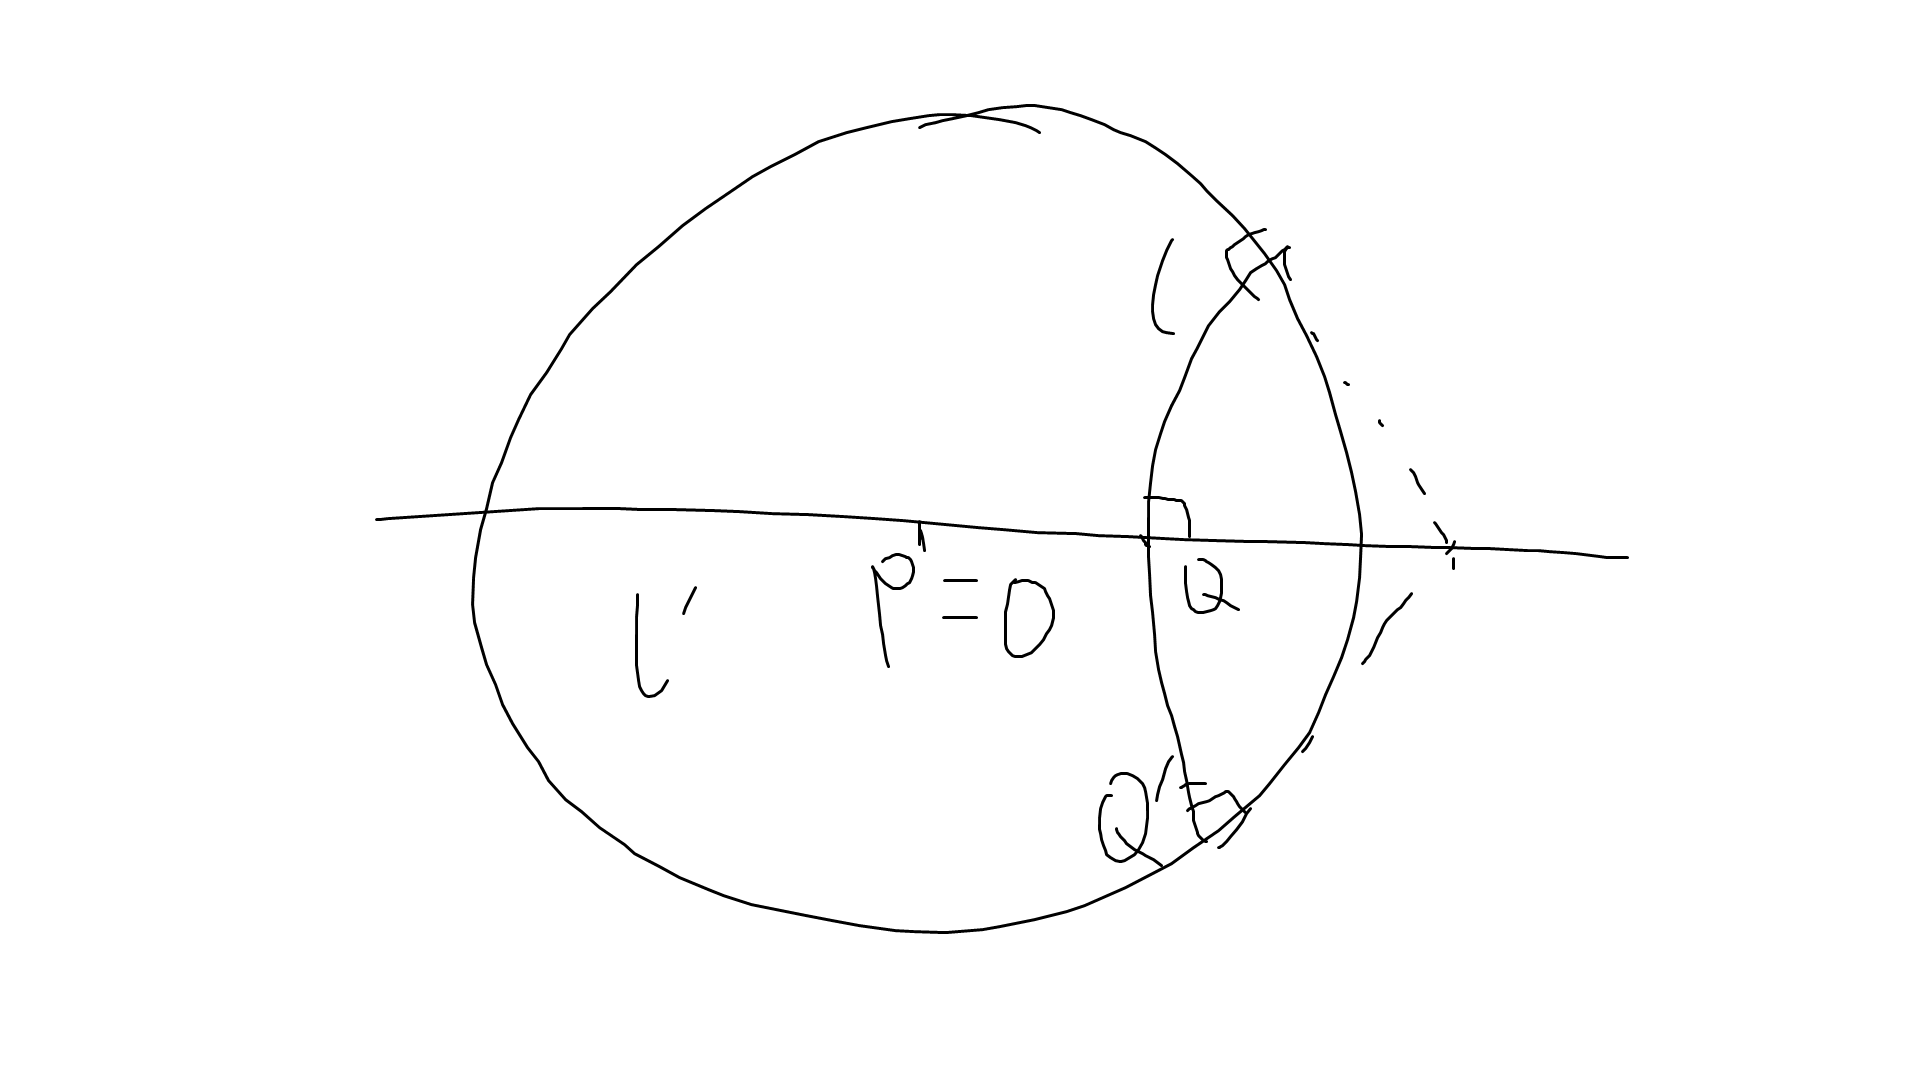
\includegraphics[scale=0.4]{Geometry_15}
\end{eg}

\begin{lemma} 4.7\\
Suppose $g$ is an isometry of $H$, and $g$ fixes every point $L^+$. Then either $g=id_H$, or $g(z) - -\bar{z}$ $\forall z \in H$, i.e. a reflection in the $y-$axis.
\begin{proof}
Let $P \in H$, $P \not\in L^+$. Then there is a unique line $l'$ through $P$ with $l' \perp L^+$, so $l'$ is a semi-circle. Let $Q=l' \cap L^+$. Then
\begin{equation*}
\begin{aligned}
\rho(P,Q) = \rho(g(P),Q)
\end{aligned}
\end{equation*}
as $g(Q)=Q$.

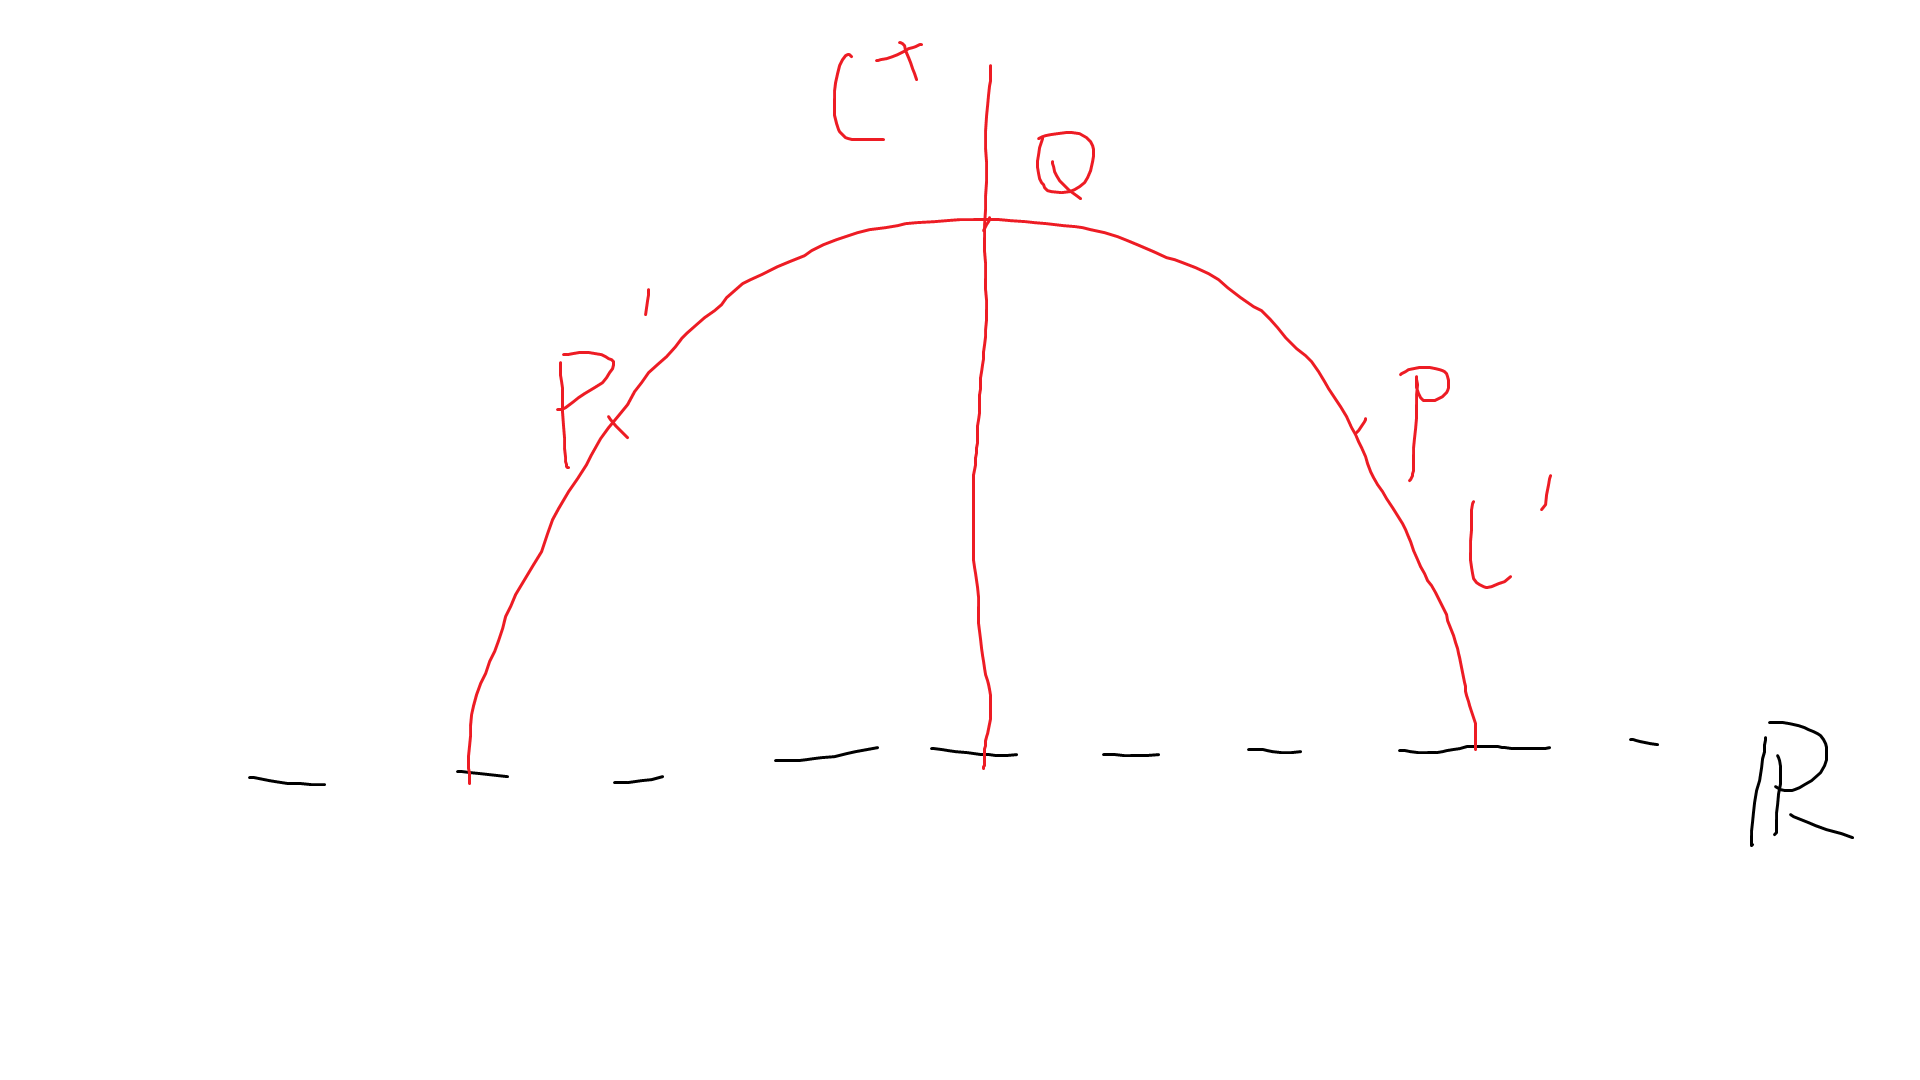
\includegraphics[scale=0.4]{Geometry_16}

Then $g(P) \in l'$ by the uniqueness of $l'$, and either $g(P) = P$ or $g(P) = P'$, where $P'$ is the image of $P$ under the reflection $z \to -\bar{z}$. Now s.t.p. if $g(P) = P$, then $g=id_H$ (for if $g(P) = P'$ then compose $g$ with $z \to -\bar{z}$ (an ieometry) to obtain $g$ is $z \to -\bar{z}$).

Let $A \neq P$, $A \not\in L^+$, $g(A) = A'$. WLOG let $P \in H^+ = \{z \in H | Re(z)>0\}$. Let $A \in H^+$.

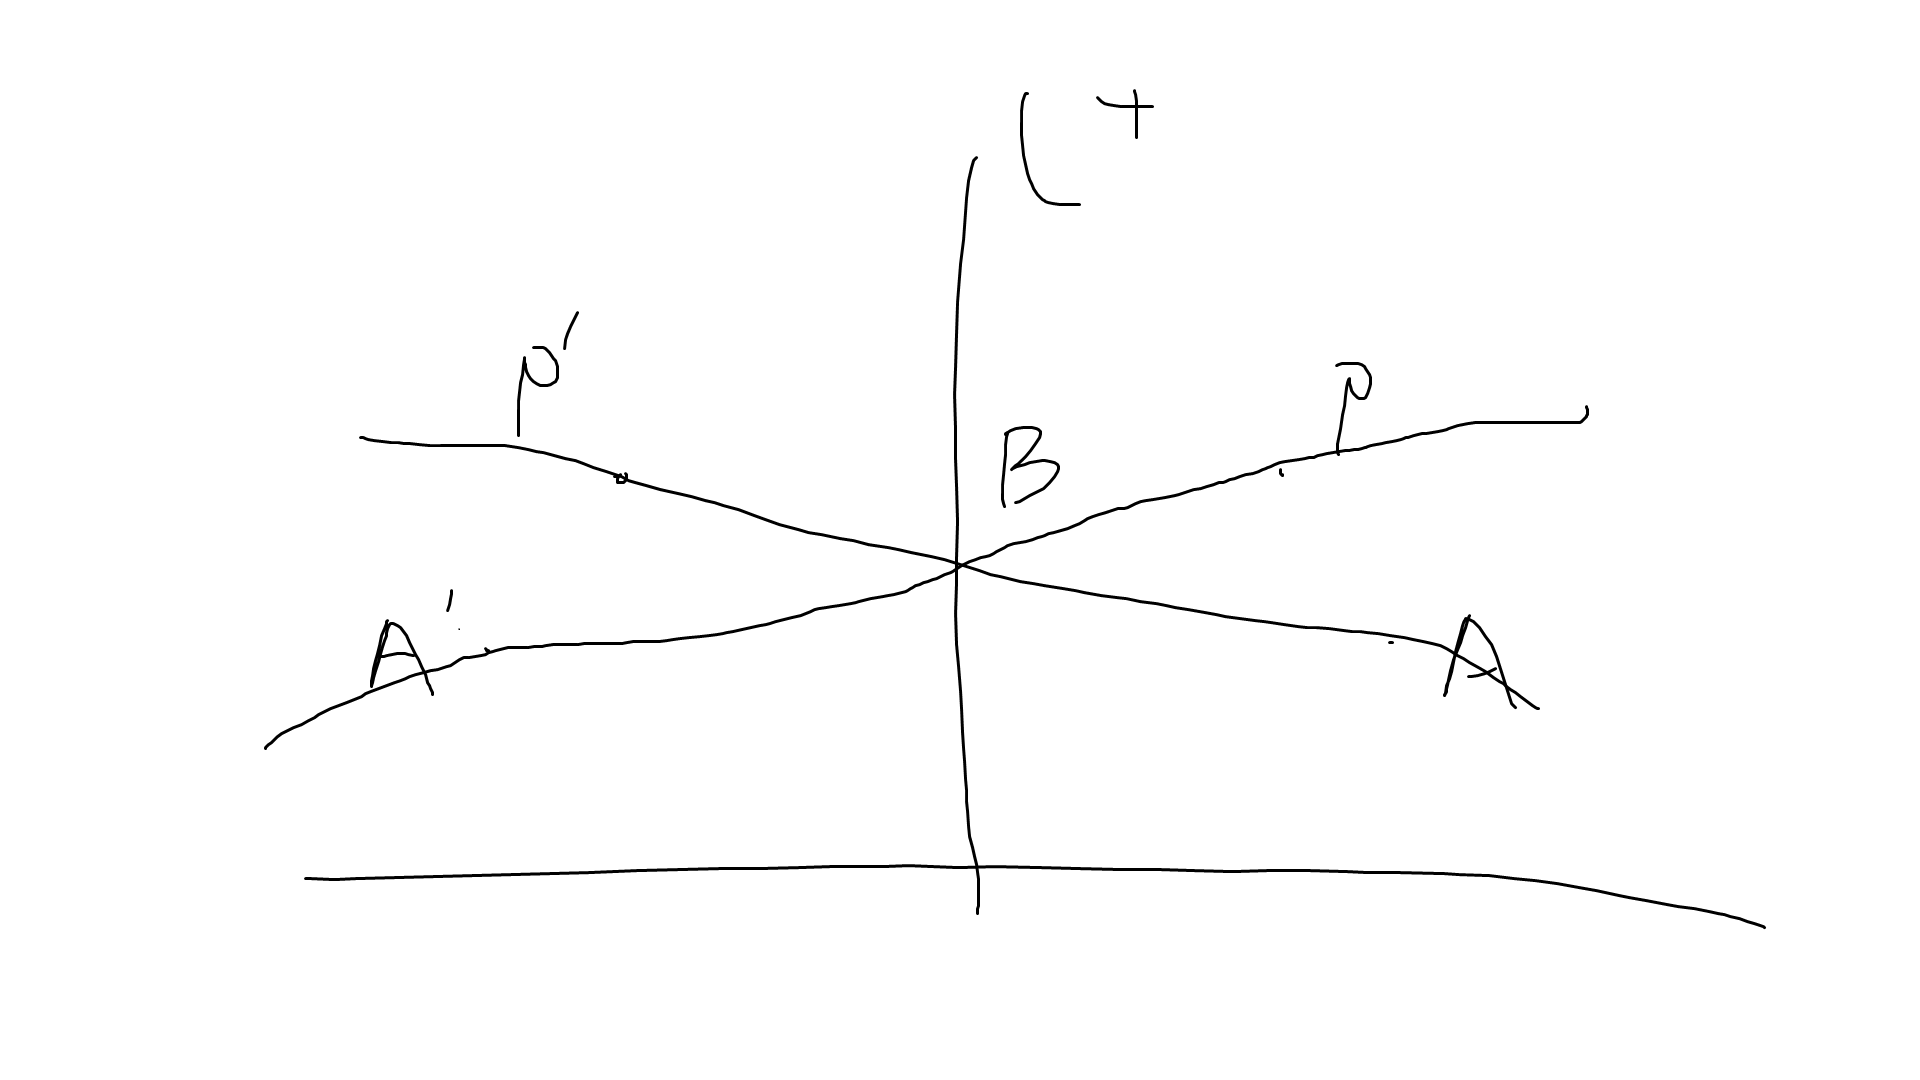
\includegraphics[scale=0.4]{Geometry_17}

then $\rho(A',P) = \rho(A,P)$ (as $g$ is isometry and $g(P)=P$). But $\rho(A',P) = \rho(A',B)+\rho(B,P) = \rho(A,B) + \rho(B,P)$, contradicts with triangle inequality $B \not\in line(AP)$. Thus $g(A)=A$, i.e. $g$ is identity.
\end{proof}
\end{lemma}

We call $R: z \in H \to -\bar{z} \in H$ the hyperbolic reflection in $L^+$, and for any hyperbolic line $l$ in $H$ with $T \in PSL(2,\R), T(l)=L^+$, call $R_l := T^{-1}RT$ the reflection (hyperbolic) in $l$.

By proposition 4.7, $R_l$ is the unique isometry fixing points in $l$ but is not the identity.

\textbf{Exercise.} Write out the reflections using the disc model.

\subsection{Hyperbolic triangles}
\begin{defi}
A hyperbolic triangle $\Delta ABC$ is the region determined by 3 hyperbolic line segments.

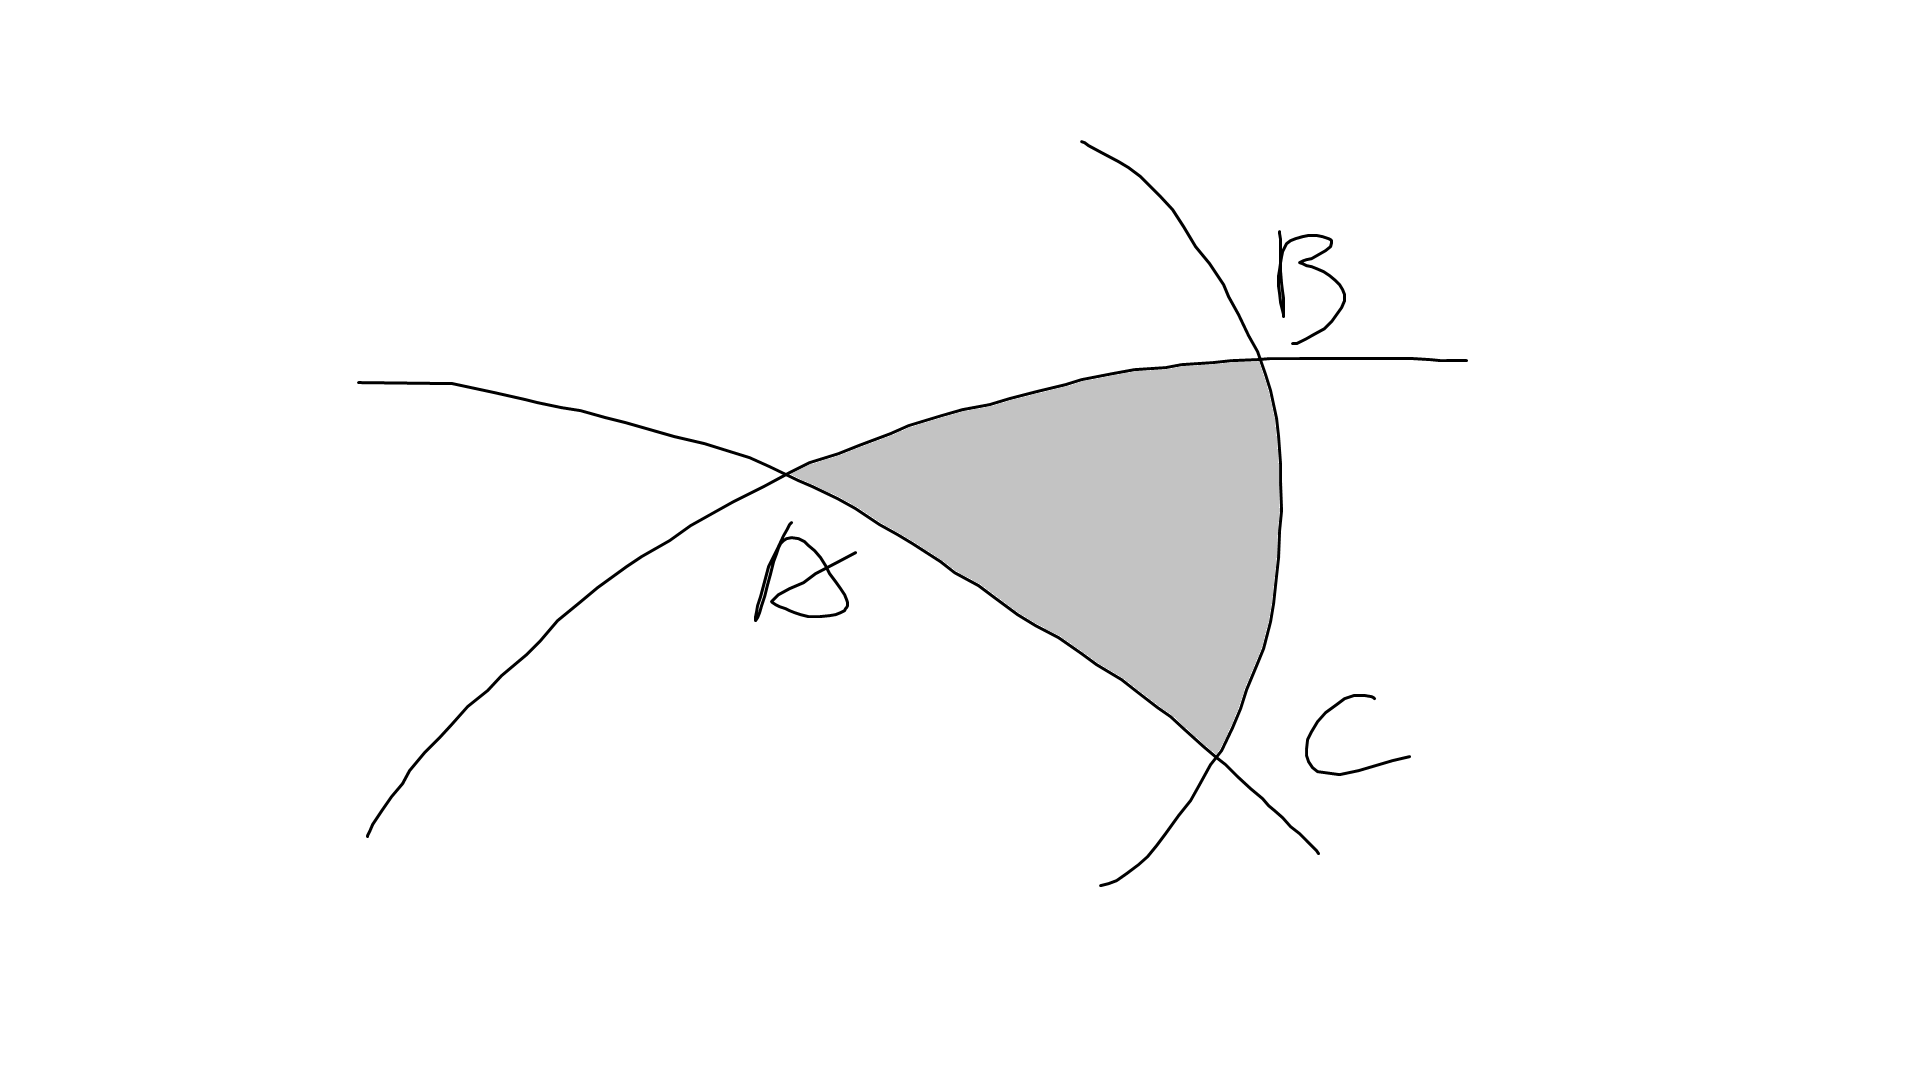
\includegraphics[scale=0.4]{Geometry_18}

Including cases when one vertex, say $A$, is at 'infinity', i.e. $A \in \R \cup \{\infty\}$ for $H$, $A \in \{|z|=1\}$ for $D$, then $\alpha = 0$.
\end{defi}

We shall prove that the area of $\Delta ABC$ = $\pi-\alpha-\beta-\gamma$.

\begin{thm} 4.8 (Gauss-Bonnet for hyperbolic triangles)\\
For each hyperbolic triangle $T=\Delta ABC$ with angles $\alpha,\beta,\gamma \geq 0$,
\begin{equation*}
\begin{aligned}
area \ T =\pi-\alpha-\beta-\gamma.
\end{aligned}
\end{equation*}
\begin{proof}
First, do the case $\gamma=0$, so $C$ is at infinity. Use the H model, WLOG let $C=\infty$ (apply ($g \in PSL(2,\R)$ if needed). Use $z \to z+a$, $a \in \R$, to centre the semicircle $AB$ at $0$ (noting $AC,BC$ are in the vertical half-lines).

Use $z \to bz$ to arche the radius of semicircle of $AB$ to be 1.

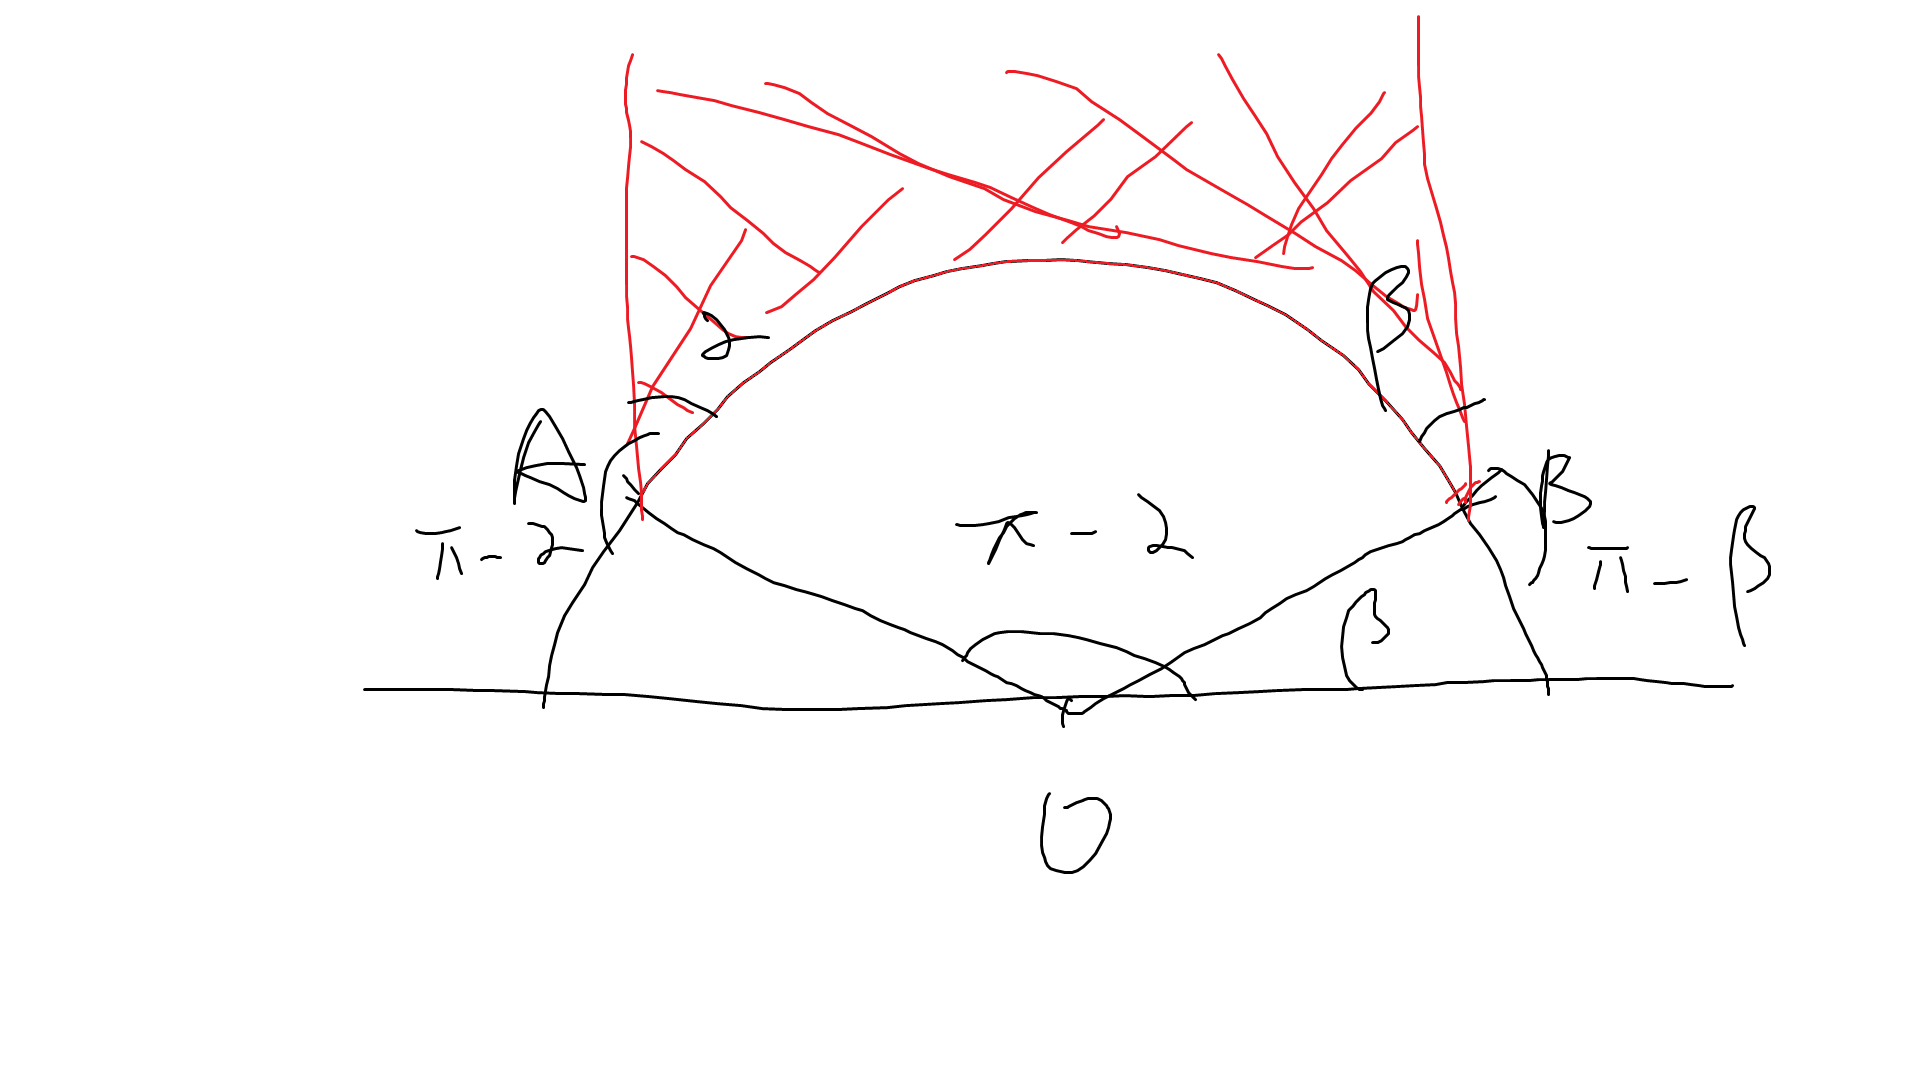
\includegraphics[scale=0.4]{Geometry_19}

Thus WLOG $AB \subset \{x^2+y^2=1,y>0\}$ and then
\begin{equation*}
\begin{aligned}
area \ T &= \int_{\cos(\pi-\alpha)}^{\cos \beta} \left(\int_{(1-x^2)^{1/2}}^\infty \frac{dy}{y^2}\right)dx\\
&= \int_{\cos(\pi-\alpha)}^{\cos\beta} \frac{dx}{(1-x^2)^{1/2}}\\
&= (-\arccos x)|_{\cos(\pi-\alpha)}^{\cos\beta} = (\pi-\alpha)-\beta
\end{aligned}
\end{equation*}
noting $\arcsin x + \arccos x = \frac{\pi}{2}$, $\arccos:[-1,1] \to [0,\pi]$, and as $\gamma=0$.

In general, using the H model again, we can apply $g \in PSL(2,\R)$ to move $AC$ into a vertical line. Then as before move (with isometry) $AB$ into a $\{x^2+y^2=1\}$ ($AC$ will remain vertical).

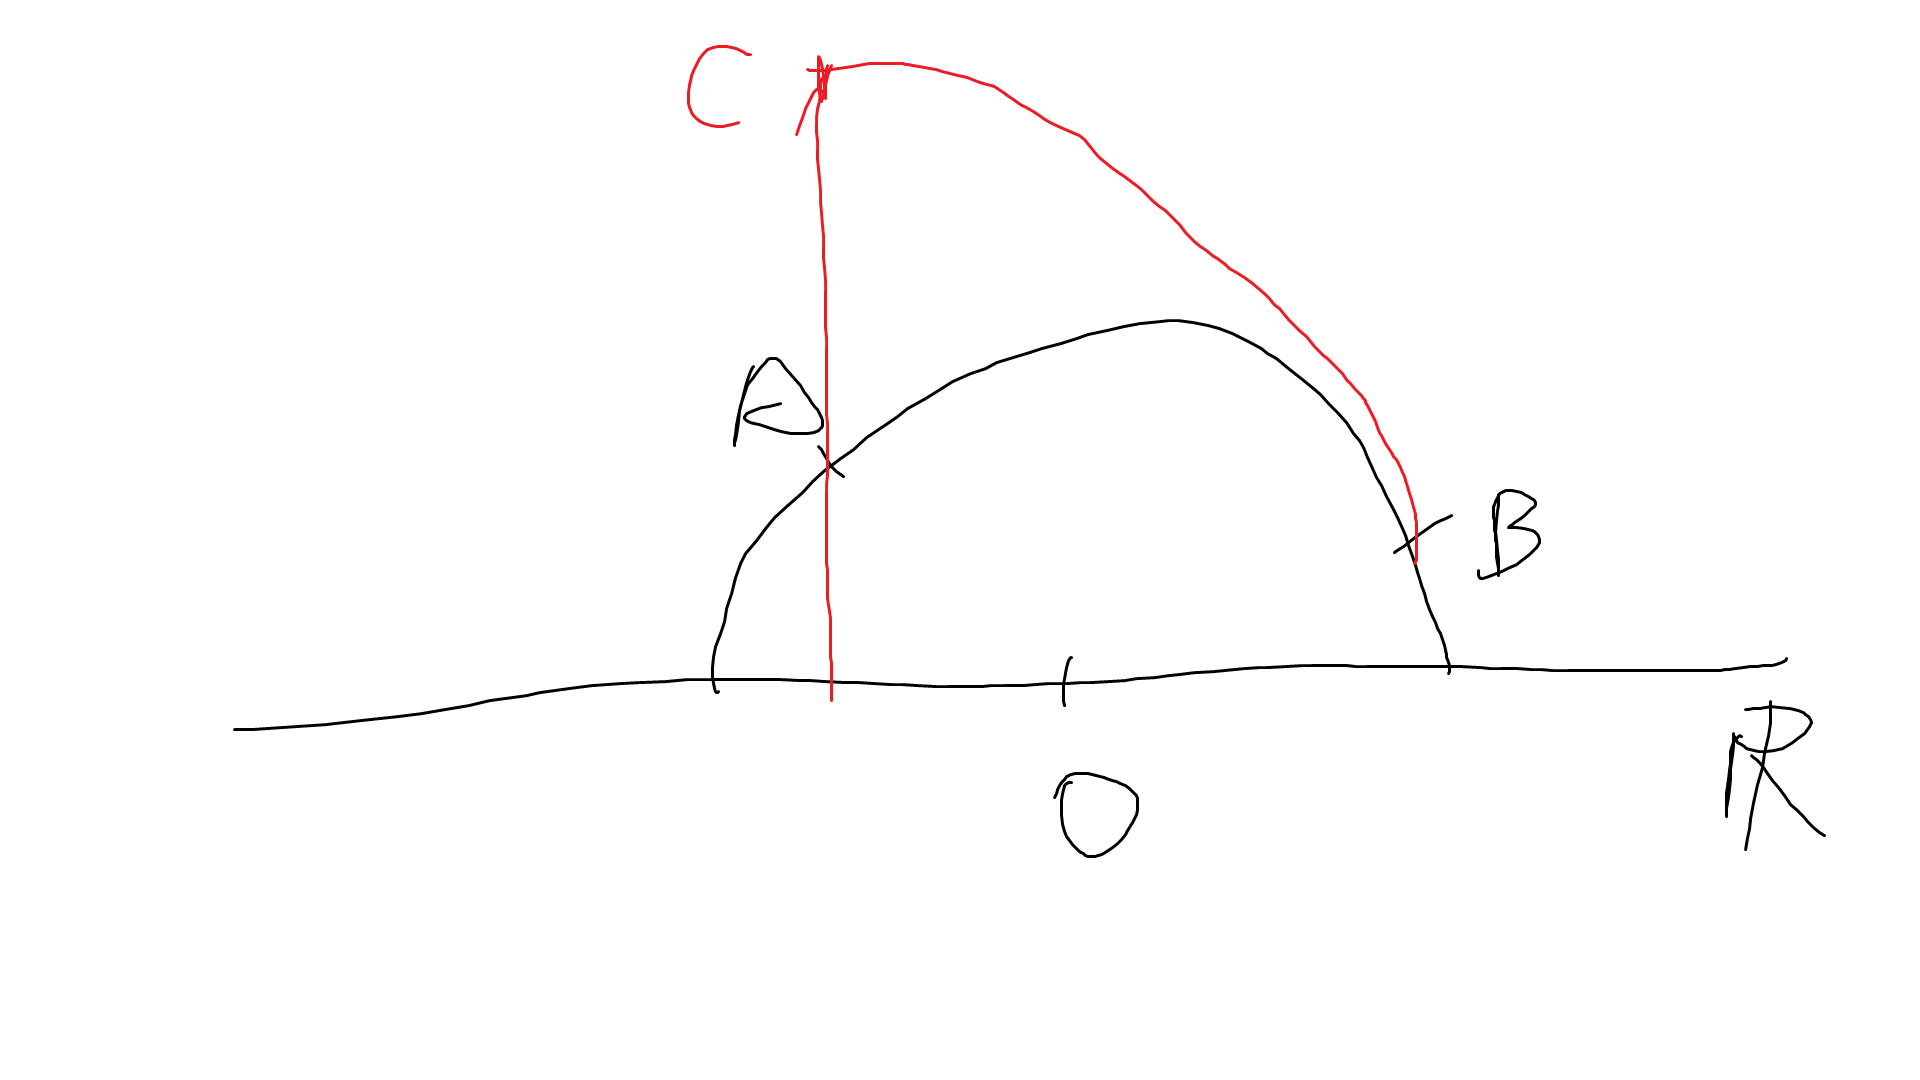
\includegraphics[scale=0.4]{Geometry_20}

Consider $\Delta_1 = AB\infty$, $\Delta_2 = BC\infty$. Then
\begin{equation*}
\begin{aligned}
area \ \Delta_1 = \pi-\alpha-(\beta+\gamma), area \ \Delta_2 = \pi-\delta - (\pi-\gamma)
\end{aligned}
\end{equation*}
So
\begin{equation*}
\begin{aligned}
area \ T &= area \Delta_1 - area \Delta_2\\
&= \pi-\alpha-\beta-\delta-\pi+\delta+\pi-\gamma\\
&= \pi-\alpha-\beta-\gamma.
\end{aligned}
\end{equation*}
\end{proof}
\end{thm}

There is hyperbolic version of sine and cosine rules (see Q16 sheet 2).

Every two lines on $S^2$ (i.e. great circles) meet, in 2 points; every two lines on $\R^2$ meet (in 1 point) if and only if they are not parallel.

\begin{defi}
Use the $D$ model of hyperbolic plane, two hyperbolic lines $l_1,l_2$ are parallel iff they only meet at $\{|\zeta| = 1\}$, and are ultraparallel iff they do not meet anywhere in $\{\zeta|\leq 1\}$.
\end{defi}

Euclid's parallel axiom (the 5th axiom) says that, given a line $l$ and $P \not\in l$, there exists unique line $l'$ s.t. $P \in l'$ with $l \cap l' = \infty$. This fails both on $S^2$ and on the hyperbolic plane -- but for a very different reason.

\subsection{Thy hyperbolic model}
Consider the \emph{Lorenzian} inner product $\left<x,y\right>$ on $\R^2$ with matrix
\begin{equation*}
\begin{aligned}
\left(\begin{matrix}
1 & 0 & 0\\
0 & 1 & 0\\
0 & 0 & -1
\end{matrix}\right)
\end{aligned}
\end{equation*}
Set $q(\mathbf{x}):=\left<x,x\right> = x^2+y^2-z^2$ for all $\mathbf{x} = (x,y,z)$. Let
\begin{equation*}
\begin{aligned}
S := \{\mathbf{x} \in \R^3 : q(\mathbf{x}) = -1\}
\end{aligned}
\end{equation*}
this is the $2$-sheet hyperboloid, with
\begin{equation*}
\begin{aligned}
S^+ = S \cap \{z>0\}
\end{aligned}
\end{equation*}
the upper sheet. Let $\pi:S^+ \to D \subset \C$ be
\begin{equation*}
\begin{aligned}
\pi(x,y,z) = \frac{x+iy}{1+z} = u+iv
\end{aligned}
\end{equation*}
the stereographic projection from $(0,0,-1)$.

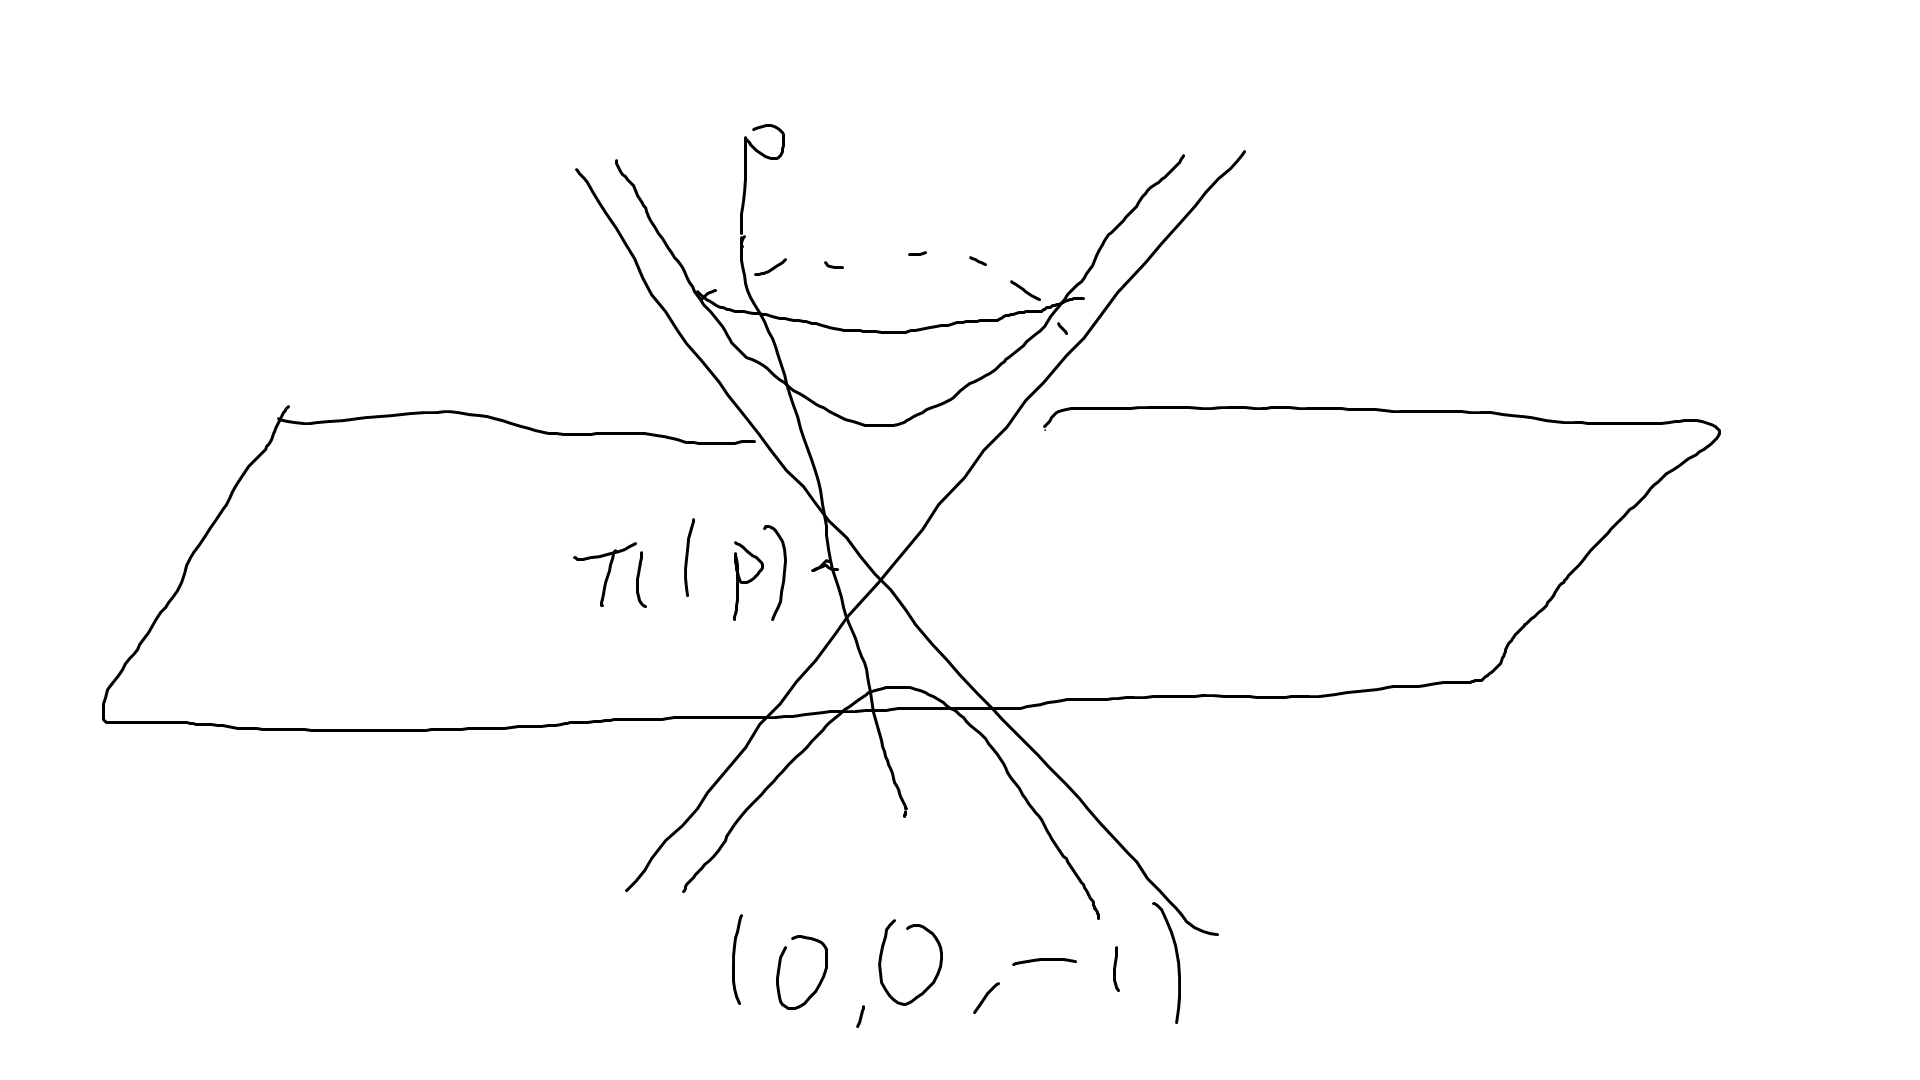
\includegraphics[scale=0.4]{Geometry_21}

Put $r^2 = u^2+v^2$, and $\sigma=\pi^{-1}: D_{u,v} \to S^+ \subset \R^3$:
\begin{equation*}
\begin{aligned}
\sigma(u,v) = \frac{1}{1-r^2} (2u,2v,1+r^2)
\end{aligned}
\end{equation*}
Now check the inner product on the tangent plane to $S^+$ at $\sigma(u,v)$ spanned by $\sigma_n:= \frac{\partial \sigma}{\partial u} = d\sigma(e_1)$, $\sigma_v = \frac{\partial \sigma}{\partial v} = d\sigma (e_2)$, $e_1,e_2$ are the standard basis of $\R^2$. Then
\begin{equation*}
\begin{aligned}
\sigma_u = \frac{2}{(1-r^2)^2} (1+u^2-v^2,2uv,2u)\\
\sigma_v = \frac{2}{(1-r^2)^2} (2uv,1+v^2-u^2,2v)
\end{aligned}
\end{equation*}
we restrict Lorenzian $\left<\cdot,\cdot\right>$ to $span\left<\sigma_u,\sigma_v\right>$ we get a symmetric bilinear form on $\R^2$ at each $(u,v) \in D$, $E du^2+2Fdudv + Gdv^2$, with
$E=\left<\sigma_u,\sigma_u\right> = \frac{4}{(1-r^2)^2}$, $F=0,G=E$,i.e.

\newpage

\section{Smooth embedded surfaces (in $R^3$)}

\begin{defi}
Let $S \subset \R^3$. $S$ is a \emph{parameterised smooth embedded surface} if each $Q \in S$ has an open neighbourhood $Q \in U = W \cap S$ for $W$ open in $R^3$ (subset topology) and a map $\sigma: V \to U$ from open $V \subset\ \R^2_{u,v}$ s.t.\\
$\bullet$ $\sigma$ is a homomorphism of $V$ onto $U$;\\
$\bullet$ $\sigma = \sigma(u,v)$ is $C^\infty$ (all partial derivatives of all orders exist and are continuous);\\
$\bullet$ at each $Q = \sigma(P)$, the vectors $\frac{\partial \sigma}{\partial u}(P), \frac{\partial \sigma}{\partial v}(P)$ are linearly independent.
\end{defi}

Now $\sigma(u,v) = \left(\begin{matrix}
x(u,v)\\
y(u,v)\\
z(u,v)
\end{matrix}\right)$. Then $$\sigma_u(P) = \frac{\partial \sigma}{\partial u}(P) = \left(\begin{matrix}
\partial x / \partial u\\
\partial y / \partial u\\
\partial z / \partial u
\end{matrix}\right)(P) = d\sigma_P(e_1), \sigma_v(P) = d\sigma_P(e_2)$$
where $e_1,e_2$ are standard basis of $\R^2$. $(u,v)$ are \emph{smooth coordinates} on $U \subset S$.

The subspace $span_\R\left<\sigma_u(P),\sigma_u(p)\right>$ is the \emph{tangent plane} $T_Q S$ to $S$ at $Q=\sigma(P)$.

$\sigma$ is a smooth ($C^\infty$) parameterisation of $U \subset S$.

\begin{prop} 5.1\\
Suppose $\sigma:V \to U$, $\tilde{\sigma}:\tilde{V} \to U$ are two $C^\infty$ parameterisations of $U$. Then the homomorphism $\varphi = \sigma^{-1} \circ \tilde{\sigma}: \tilde{V} \to V$ is a diffeomorphism.
\begin{proof}
It suffices to consider $\varphi$ on a small neighbourhood of some $P = (u_0,v_0) \in \tilde{V}$. The Jacobi matrix of $\left(\begin{matrix}
x_u & x_v\\
y_u & y_v\\
z_u & z_v
\end{matrix}\right)$ has rank 2 for each $(u,v) \in V$ by the definition of $\sigma$. WLOG let $(x_u,x_v)$ and $(y_u,y_v)$ be linearly indepnedent at $(u_0,v_0)$. Let $F(u,v) = \left(\begin{matrix}
x(u,v)\\
y(u,v)
\end{matrix}\right)$. Then by inverse function theorem (from Analysis II), $F$ maps some open neighbourhood of $(u_0,v_0) \in N$ diffeomorphically onto the image (open) $N' \subset \R^2$. Now $\sigma(N)$ is open, $\tilde{N} \subset U = \tilde{\sigma}^{-1} (\sigma(N)) \subset \tilde{V}$ is open (by homomorphism property). $\sigma_1 F$ is bijective, so $\pi = F \circ \sigma^{-1}$ is also bijective. So $\tilde{F} = \pi \circ \tilde{\sigma}$.

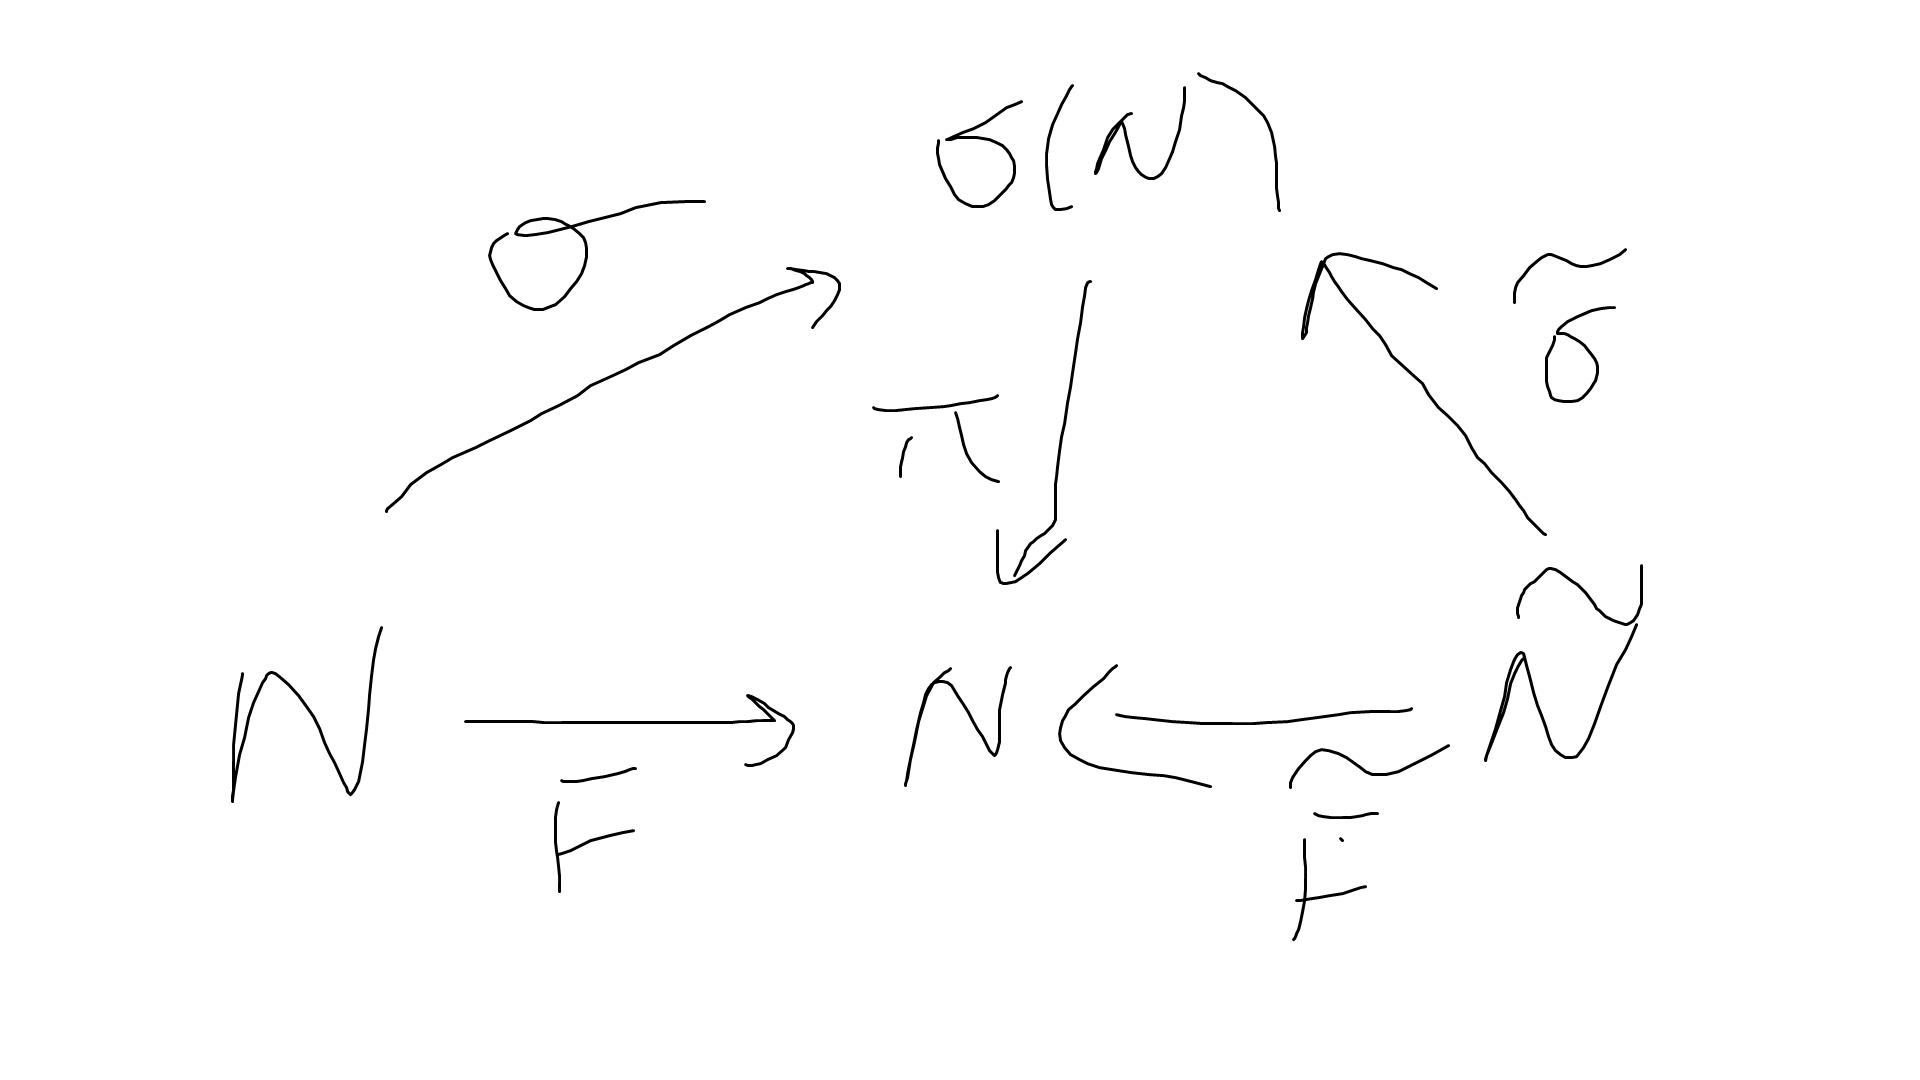
\includegraphics[scale=0.3]{Geometry_22}

Furthermore, $\pi(x,y,z) = (x,y)$ is certainly smooth since it's a linear map. Now $\varphi = \sigma^{-1} \circ \tilde{\sigma} = \sigma^{-1} \circ \pi^{-1} \circ \pi \circ \tilde{\sigma} = F^{-1} \circ \tilde{F}$ on $\tilde{N}$ a smooth map as $F^{-1}$ and $\tilde{F}$ are so. By symmetry, $\varphi^{-1}$ is also $C^\infty$ on $N$. So done.
\end{proof}
\end{prop}

\begin{coro}
the tangent plane $T_Q S$ is independent of the choice of parameterisation $\sigma$.
\begin{proof}
Let $\tilde{\sigma}(\tilde{u},\tilde{v}) = \sigma(\varphi(\tilde{u},\tilde{v}),\varphi_2(\tilde{u},\tilde{v}))$, $\varphi = (\varphi_1,\varphi_2)$. By chain rule, $$\tilde{\mathbf{\sigma}}_{\tilde{u}} =(\varphi_1)_{\tilde{u}} \mathbf{\sigma}_u + (\varphi_2)_{\tilde{u}}\mathbf{\sigma} v,\\ 
\tilde{\mathbf{\sigma}}_{\tilde{v}} =(\varphi_1)_{\tilde{v}} \mathbf{\sigma}_u + (\varphi_2)_{\tilde{v}}\mathbf{\sigma} v$$. Then the Jacobi matrix for $\varphi$ is
\begin{equation*}
\begin{aligned}
J(\varphi)=\left(\begin{matrix}
\varphi_{1,\tilde{u}} & \varphi_{2,\tilde{u}}\\
\varphi_{1,\tilde{v}} & \varphi_{2,\tilde{v}}
\end{matrix}\right)
\end{aligned}
\end{equation*}
which is invertible as $\varphi$ is a diffeomorphism.
\end{proof}
\end{coro}

\begin{rem}
We can compute $\tilde{\mathbf{\sigma}}_{\tilde{u}} \times \tilde{\mathbf{\sigma}}_{\tilde{v}} = \det(J\varphi) \sigma_u \times \sigma_v$.
\end{rem}

\begin{defi}
The \emph{unit normal} to $S$ at $Q$ is 
\begin{equation*}
\begin{aligned}
N = N_Q := \frac{\sigma_u \times \sigma_v}{||\sigma_u \times \sigma_v||}
\end{aligned}
\end{equation*}
Note that $N$ is well-defined up to a sign.

$\theta:= \sigma^{-1}: U \subset S \to V \subset \R^2$ is called a \emph{chart}.
\end{defi}

\begin{eg}
Consider on $S^2$ the two stereographic projections from the North and South poles; they are both charts with domains covering $S^2$.
\end{eg}

If $S \subset \R^3$ is an embedded surface, then each $T_Q S$ ($Q \in S$ inherits an inner product from $\R^3$ - i.e. we get a \emph{family} of inner products depending on $Q \in S$. This family is the \emph{first fundamental form of $S$}.

Given a parameterisation $\sigma: V \to U \subset S$ and $P \in V$, $a,b \in \R^2$, $\left<a,b\right>_P:=\left<d\sigma_P(a),d\sigma_P(b)\right>_{\R^3}$ w.r.t. standard basis $e_1,e_2$ of $\R^2$, the RHS becomes $E du^2 +2Fdudv+Gdv^2$ with $E = \left<\sigma_u,\sigma_u\right>_{\R^3}$, $F = \left<\sigma_u,\sigma_v\right>_{\R^3}$, $G = \left<\sigma_v,\sigma_v\right>_{\R^3}$. Here $\sigma_u = d\sigma (e_1)$, $\sigma_v = d\sigma (e_2)$.

This Riemannian metric of $V$ is also called the first fundamental form w.r.t $\sigma$ (especially in practical examples).

Fact: if $\tilde{\sigma} = \sigma \circ \varphi: \tilde{V} \to \tilde{U}$ as in proposition 5.1, then $\varphi$ is an isometry of the respective Riemannian metric on $V $ and $\tilde{V}$.

\begin{defi}
Given a smooth curve $\Gamma:[a,b] \to S \subset \R^3$,
\begin{equation*}
\begin{aligned}
length(\Gamma) := \int_a^b ||\Gamma'(t)|| dt\\
energy(\Gamma) := \int_a^b ||\Gamma'(t)||^2 dt.
\end{aligned}
\end{equation*}
\end{defi}

When $\Gamma([a,b]) \subset U = \sigma(V)$, then there exists unique $\gamma:[a,b] \to V$ open in $\R^2$ s.t. $\Gamma = \sigma \circ \gamma$ (we use these coordinates in $\R^2$ to express the curve in terms of $u$ and $v$). So $\gamma=(\gamma_1,\gamma_2)$, $\Gamma'(t) = (d\sigma)_{\gamma(t)} (\dot{\gamma}_1 (t) e_1 + \dot{\gamma}_2(t) e_2) = \dot{\gamma}_1 \sigma_u + \dot{\gamma}_2 \sigma v$. So
\begin{equation*}
\begin{aligned}
length(\Gamma) = \int_a^b \left(E \dot{\gamma}_1^2 + 2F\dot{\gamma}_1\dot{\gamma}_2 + G\dot{\gamma}_2^2\right)^{1/2} dt
\end{aligned}
\end{equation*}

\begin{defi}
Given a $C^\infty$ parameterisation $\sigma:V \to U \subset S$ of surface $S$ and a region $T \subset U$. Then 
\begin{equation*}
\begin{aligned}
area(T) = \int_{\theta(T)} (EG-F^2)^{1/2} dudv
\end{aligned}
\end{equation*}
where $\theta(T) = \sigma^{-1}$ is the respective \emph{chart}.
\end{defi}

\begin{prop} 5.3\\
The area is well defined, i.e. $area(T)$ is independent of the partamerisation $\sigma$. Thus we may extend the definition of $area(T)$ to more general $T$ which is not necessarily contained in one parameterized neighbourhood.
\end{prop}

\begin{rem}
In practical examples, $\sigma(V) = U$ is often \emph{dense} in $S$. Then it suffices to use just this $U$ to compute $area(S)$.

Areas and lengths are invariant under isometries.
\end{rem}

\newpage

\section{Geodesics}

Let $V \subset \R^2_{u,v}$ open and we are given a Riemannian metric $Edu^2+2Fdudv+Gdv^2$. Suppose $\gamma=(\gamma_1,\gamma_2):[a,b] \to V$ is a $C^\infty$ curve.

\begin{defi}
$\gamma$ is a \emph{geodesic} if:\\
(1) $\frac{d}{dt} (E \dot{\gamma}_1 + F \dot{\gamma}_2 ) = \frac{1}{2} (E_u \dot{\gamma}_1^2 + 2 F_u \dot{\gamma}_1 \dot{\gamma}_2 + G_u \dot{\gamma}_2^2 )$ and\\
(2) $\frac{d}{dt}(F \dot{\gamma}_1 + G\dot{\gamma}_2) = \frac{1}{2}(E_v \dot{\gamma}_1^2 + 2F_v \dot{\gamma}_1 \dot{\gamma}_2 + G_v \dot{\gamma}_2^2)$\\
hold for all $t \in [a,b]$.
\end{defi}

Let $\gamma(a) = p$, $\gamma(b) = q$. A \emph{proper variation} of $\gamma$ is a $C^\infty$ map $h:[a,b] \times (-\varepsilon,\varepsilon) \to V \subset \R^2$ s.t. $h(t,0) = \gamma(t)$, $t \in [a,b]$, $h(a,\tau) = p$, $h(b,\tau) = q$ for all $\tau \in (-\varepsilon,\varepsilon)$. So for all $\tau$, $\gamma_\tau:[a,b] \to V$, $\gamma_\tau = h(t,\tau)$ is a $C^\infty$ curve.

\begin{prop} 6.1\\
$\gamma$ satisfies the geodesic ODEs iff $\gamma$ is the stationary point of for the energy function for all proper variations, i.e. $\frac{d}{d\tau}|_{\tau=0} E(\gamma_\tau) = 0$.
\begin{proof}
We write $\gamma(t) = (i(t),v(t))$. Then
\begin{equation*}
\begin{aligned}
energy(\Gamma) &= \int_a^b \left(E(u,v) \dot{u}^2 + 2F(u,v) \dot{u}\dot{v} + G(u,v) \dot{v}^2\right) dt\\
&= \int_a^b I(u,v,\dot{u},\dot{v} dt.
\end{aligned}
\end{equation*}

Euler-Lagrange equations: a solution $\gamma$ is stationary iff
\begin{equation*}
\begin{aligned}
\frac{d}{dt} \left(\frac{\partial I}{\partial \dot{u}}\right) = \frac{\partial I}{\partial u},\\
\frac{d}{dt} \left(\frac{\partial I}{\partial \dot{v}}\right) = \frac{\partial U}{\partial v}
\end{aligned}
\end{equation*}
But LHS of the first equation is just $2E\dot{u}+2F \dot{v}$ and RHS is $e_u \dot{u}^2 + 2F_u \dot{u} \dot{v} + G_u \dot{v}^2$. So we get the first geodesic equation. The second is obtained similarly.
\end{proof}
\end{prop}

Now let $S \subset \R^3$ be an embedded surface. $\sigma: V \to U \subset S$ a parameterisation, $\theta = \sigma^{-1}:U \to V$ the chart, and let $\Gamma:[a,b] \to S$ a smooth curve in $S$, $\gamma = \theta\circ \Gamma$ a smooth curve in $V$.

Define $\Gamma$ to be a \emph{geodesic} on $S$ iff $\gamma$ is a geodesic in $V$, i.e. iff $\Gamma$ is a startionary point of $\int_a^b ||\Gamma'(t)||^2 dt$. This is independent of choice of $\sigma$.

\begin{coro} 6.2\\
If a curve $\Gamma$ in $S$ minimizes the energy among all the curves with the same end-points, then $\Gamma$ is a geodesic.
\begin{proof}
Let $\Gamma:[a,b] \to S$. For all $a<a_1<b_1<b$, $\Gamma_1 = \Gamma|_{[a_1,b_1]}$ then minimizes the energy among all curves from $\Gamma(a_1)$ to $\Gamma(b_1)$.

If $a_1,b_1$ are such that $\Gamma[(a_1,b_1]) \subset U$ for some parameterized neighbourhood, then $\Gamma_1$ must be a geodesic by proposition 6.1, $\Gamma_1$ is a geodesic. Now vary $a_1,b_1$ to get a cover of $[a,b]$.
\end{proof}
\end{coro}

\begin{lemma} 6.3\\
Let $V \subset \R^2$, $P,Q \in V$, $V$ is endowed with a Riemannian metric. Consider $C^\infty$ curve $\gamma_0$, $\gamma_0(0) = P$, $\gamma_0(1) = Q$. Then $\gamma_0$ minimizes the energy iff $\gamma_0$ minimizes the length and has constant speed $\dot{\gamma}_0$.
\begin{proof}
Cauchy-Schwartz for $f,g\in C[0,1]$ says
\begin{equation*}
\begin{aligned}
\left(\int_0^1 fg\right)^2 \leq \int_0^1 f^2\int_0^1 g^2
\end{aligned}
\end{equation*}
with equality attained iff $g=\lambda f$ for some $\lambda \in \R$, or alternatively $f=0$.

Put $f \equiv 1$, $g = ||\dot{\gamma}||$. Then
\begin{equation*}
\begin{aligned}
(length(\gamma))^2 \leq energy(\gamma)
\end{aligned}
\end{equation*}
with equality attained only if $||\dot{\gamma}||$ is a constant.

If $length(\gamma) = l$, then the minimum of energy $l^2$ does occur exactly when $||\dot{\gamma}||$ is a constant.
\end{proof}
\end{lemma}

\begin{rem}
We can show that a curve $\gamma$ is geodesic precisely if $\Gamma$ locally minimizes energy, also iff $\gamma$ locally minimizes length and has constant speed. By locally minimizing we mean that $\forall t_0$, $\exists \varepsilon > 0$ s.t. $\gamma|_{t_0-\varepsilon,t_0+\varepsilon]}$ minimizes length/energy.
\end{rem}

\begin{rem}
Geodesic ODEs actually imply $||\Gamma'(t)||$ is a constant (see example sheet 3 Q7).
\end{rem}

Further properties of the geodesics:

Recall that the defining ODEs are of the form
\begin{equation*}
\begin{aligned}
\frac{d}{dt} \left(\left(\begin{matrix}
E & F\\
F & G
\end{matrix}\right)\left(\begin{matrix}
\dot{u}\\
\dot{v}
\end{matrix}\right)\right) = \text{ terms with derivative of lower order}
\end{aligned}
\end{equation*}
The matrix $\left(\begin{matrix}
E & F\\
F & G
\end{matrix}\right)$ is invertible, thus the ODE is of the form $(\ddot{u},\ddot{v}) = \mathcal{F}(u,v,\dot{u},\dot{v})$. Standard theory of ODEs (Analysis II, application of the contraction mappings) show that for all $P=(u_0,v_0) \in V \subset \R^2$, for all $\mathbf{a} = (p_0,q_0) \in \R^2$, there exists unique geodesic $\gamma(t) = (u(t),v(t))$, for $|t|<\varepsilon$, with $\gamma(0) = P$, $\dot{\gamma}(0) = \mathbf{a}$.

\begin{eg}
Consider $S^2 \subset \R^3$, for all $P \in S^2$, all tangent direction (at $P$), there exists a unique great circle.

As arcs of great circles of length $<\pi$ are length minimizing, we find from Corollary 6.2 and Lemma 6.3, that the great circles are \emph{all} the geodesics on $S^2$.

Similarly, on the hyperbolic plane, the hyperbolic lines are \emph{all} the geodesics.

This can also be verified directly -- see Q7 sheet 3.
\end{eg}

We can use the geodesics on a surface $S \subset \R^3$ to construct around each point $P \in S$ the \emph{geodesic polar coordinates} (a coordinate chart simplifying the coefficients of the first fundamental form($E,F,G$)).

Sketch of proof:\\
Solutions of the geodesic ODEs depend on $C^\infty$ on the initial conditions.\\
Let $\psi:U \to V \subset \R^2$ where $V$ is open, and a coordinate chart $P \in U \subset S$ where $U$ is open, and $\psi(P) = 0 \in V$.

For all value $\theta$, there exists a unique geodesic $\gamma^\theta:(-\varepsilon,\varepsilon) \to V$ with $\gamma^\theta(0) =0$, $\dot{\gamma}^\theta(0) = $the unit vector in the direction of $|tehta$.

Set $\sigma(r\theta) := \gamma^\theta(r)$. We can show:\\
1) $\sigma$ is smooth in $(r,\theta)$;\\
2) For all $\theta_0$, $\psi^{-1} \circ \sigma: \{(r,\theta): 0 < r < \varepsilon, \theta_0 < \theta < \theta_0+2\pi\} := W \to S$, i.e. $\sigma: W \to V \setminus\{0\}$, $\\psi^{-1}: V \setminus\{0\} \to U \setminus\{P\} \subset S$.

$\psi^{-1} \circ \sigma$ is a valid parameterisation, so $\sigma^{-1} \circ \psi$ is a valid \emph{chart}.

The values $(r,\theta)$ of this chart are the \emph{geodesic polar coordinates} at $P$.

Gauss lemma says the geodesic circles $\{r = r_0\} \subset W$ are perpendicular to their radii, i.e. to $\gamma^\theta$, and the Riemmanian metric on $W$ is
\begin{equation*}
\begin{aligned}
dr^2 + G(r,\theta)d\theta^2.
\end{aligned}
\end{equation*}

An \emph{atlas} is a collection of charts (with domains) covering $S$. For example, geodesic polar coordinates define an atlas.

Other good atlases are given in sheet 3 (for $S = S^2$).

\subsection{Surface of Revolution}
We consider $S \subset \R^3$ that can be obtained by rotating a plane curve $\eta$ around a straight line $l$.

WLOG let $l$ be the $z-$axis and $\eta$ in the $(x,z)-$plane, i.e.
\begin{equation*}
\begin{aligned}
\eta:(a,b) \subseteq \R, \eta(u) = (f(u),0,g(u)).
\end{aligned}
\end{equation*}

We require:\\
(1) $||\eta'(u)|| = 1$ for all $u$. This basically requires the 'velocity' to be 1, and can be always obtained by parameterising using length;\\
(2) $f(u)>0$;\\
(3) $\eta$ is a homomorphism onto its image. This rules out some weird examples that we don't want, for example,

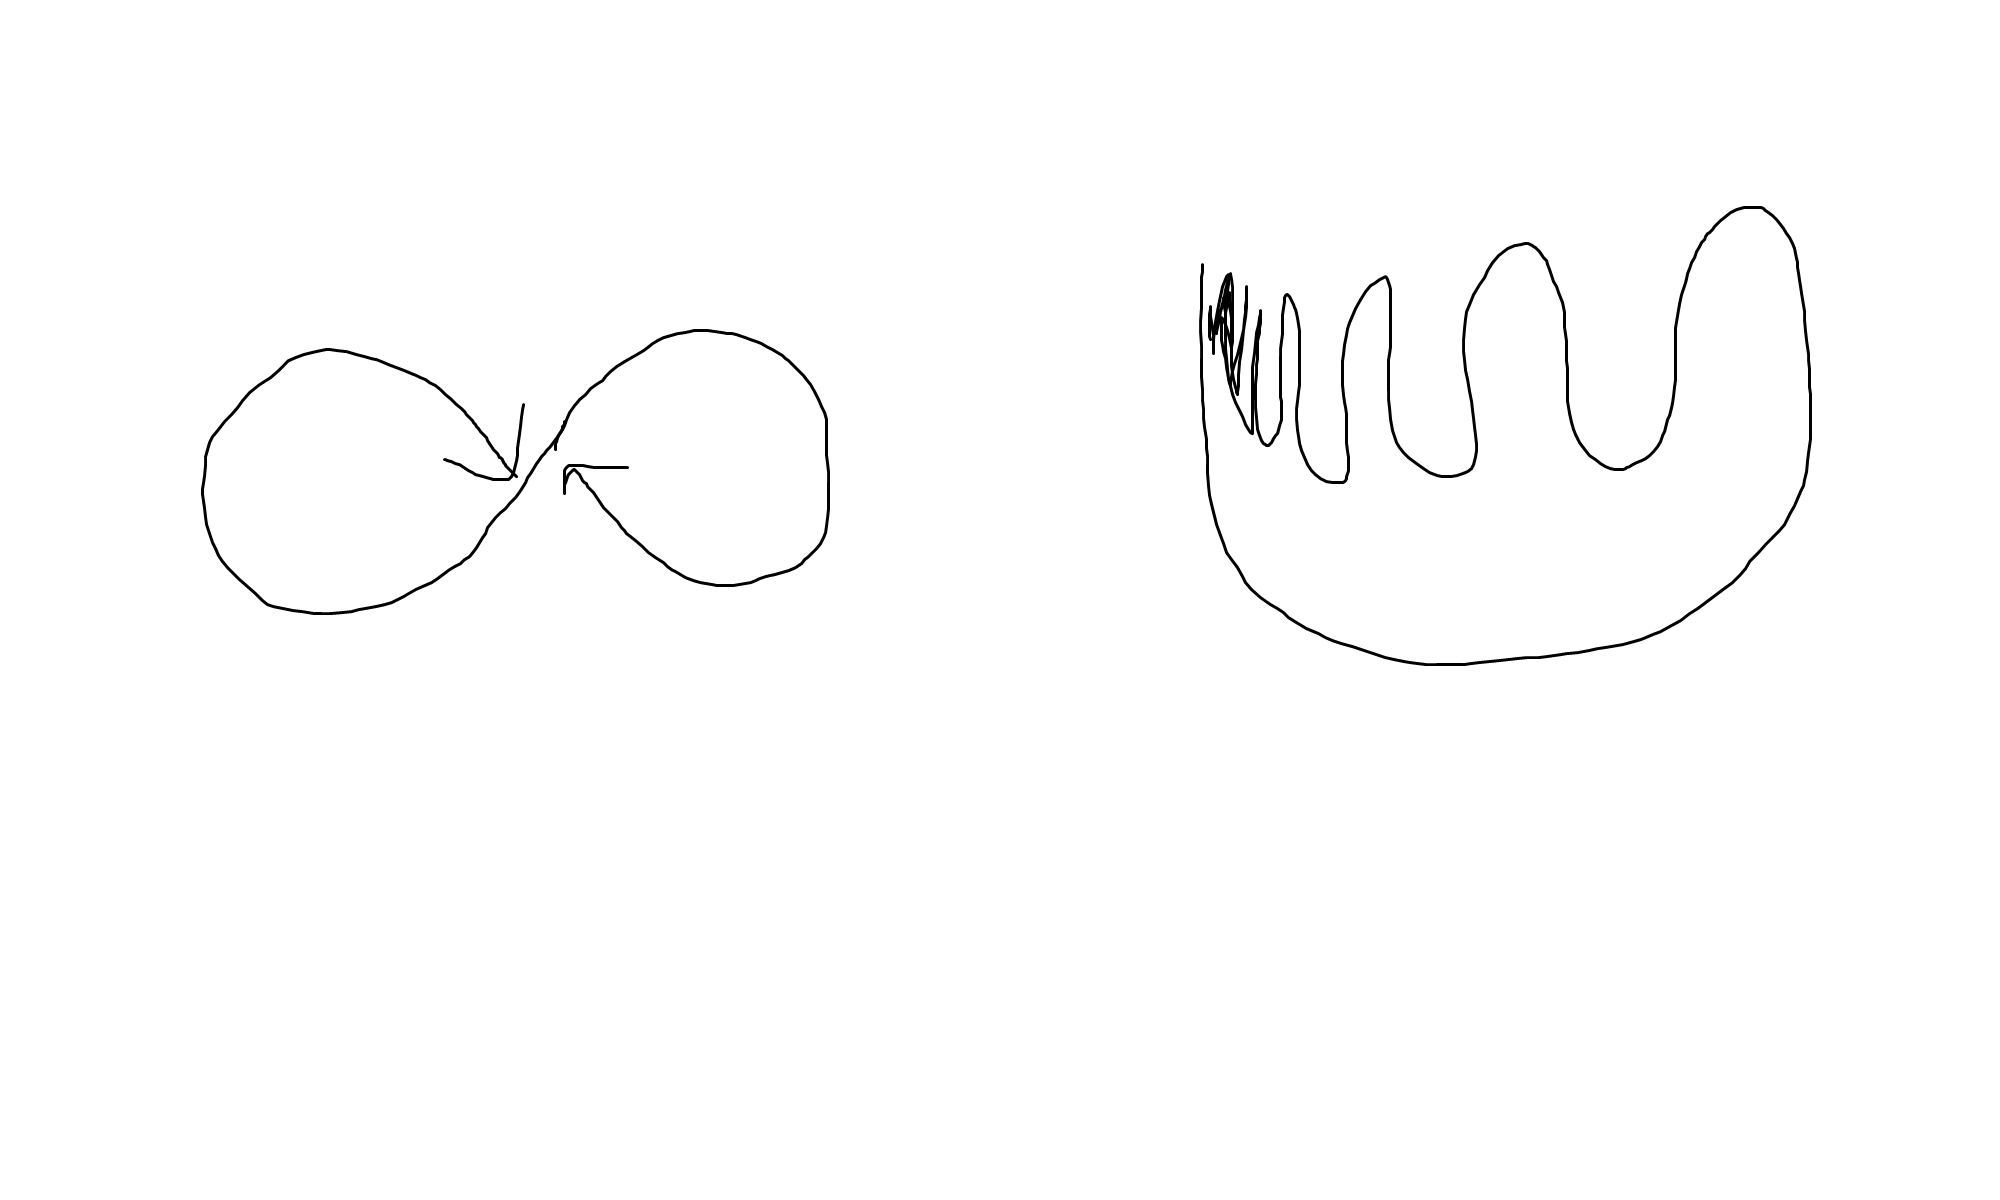
\includegraphics[scale=0.4]{Geometry_23}

Define $S$ as the image of $\sigma(u,v) = (f(u) \cos v, f(u) \sin v, g(u))$, $a<u<b$, $0 \leq v \leq 2\pi$, and for all $\alpha \in \R$, $\sigma^\alpha:(a,b) \times (\alpha,\alpha+2\pi)$ is a homomorphism onto its image (see Q1 sheet 3). Then
\begin{equation*}
\begin{aligned}
\sigma_u^\alpha = (f'\cos v, f'\sin v, g'),\\
\sigma_v^\alpha = (-f\sin v, f\cos v, 0)
\end{aligned}
\end{equation*}
so
\begin{equation*}
\begin{aligned}
\sigma_u \times \sigma_v =(-fg'\cos v, -fg' \sin v, ff'),\\
||\sigma_u^\alpha \times \sigma_v^\alpha||^2 = f^2(f'^2+g'^2) = f^2 > 0 (\neq 0)
\end{aligned}
\end{equation*}
Thus $\sigma^\alpha$ is a valid parameterisation. so $S$ is a valid embedded surface. The first fundamental form w.r.t. $\sigma^\alpha$ is
\begin{equation*}
\begin{aligned}
E &= ||\sigma_u||^2 = f'^2+g'^2 = 1,\\
F &= \sigma_u \cdot \sigma_v = 0,\\
G &= ||\sigma_v||^2 = f^2.
\end{aligned}
\end{equation*}
So the Riemannian metric is $du^2 + f^2 dv^2$.

\begin{defi}
Curves on $S$ of the form $\gamma(t) = \sigma(t,v_0)$ are called \emph{meridians}, $\gamma(t) = \sigma(u_0,t)$ are called \emph{parallels}.
\end{defi}

Then the geodesic ODEs for $\gamma=(u,v)$ in $V \subset \R^2$ are
\begin{equation*}
\begin{aligned}
\left\{\begin{array}{ll}
\ddot{u} &= f \cdot \frac{df}{du} \cdot \dot{v}^2\\
\frac{d}{dt}(f^2 \dot{v}) &= 0
\end{array}\right.
\end{aligned}
\end{equation*}

\begin{prop} 6.4\\
Assume $||\dot{\gamma}||=1$, i.e. $\dot{u}+f^2(u)\dot{v}^2=1$. Then\\
(i) Every unit speed meridian $\gamma(t) = \sigma(t,v_0)$ is a geodesic;\\
(ii) A unit speed parallel $\gamma(t) = \sigma(u_0,t)$ is a geodesic precisely when $\frac{df}{du}(u_0)=0$, i.e. $u_0$ is a stationary point.
\begin{proof}
(i) $v=v_0=$constant. So the second equation holds. Also we have $\dot{u}$ is a constant since $\dot{v} = 0$. So the first equation holds as well.\\
(ii) $u=u_0=$constant so $||\dot{\gamma}||^2 = f^2(u_0) \dot{v}^2 = 1$. So $\dot{v} = \pm \frac{1}{f(u_0)} \neq 0$ is a constant. Then the second equation holds. Now the first equation only holds if $\frac{df}{du}(u_0) = 0$ as $\ddot{u} = 0$.
\end{proof}
\end{prop}

\newpage

\section{Gaussian Curvature}
Recall the curves $\eta:[0,l] \to \R^2$ a $C^\infty$ curve with $||\eta'||=1$. Recall the curvature $\kappa$ at $\eta(s)$ is determined by
\begin{equation*}
\begin{aligned}
\eta'' = \kappa \mathbf{n}
\end{aligned}
\end{equation*}
where $\mathbf{n}$ is a norm along $\eta$ ($\mathbf{n} \cdot \eta'=0$, $||\\mathbf{n}=1$, and $\kappa \geq 0$.

Let $f:[c,d] \to [0,l]$ be smooth, $f'(t)>0$, so we may reparameterize $\gamma(t) = \eta(f(t))$. Then $\dot{\gamma} = \dot{f}\cdot \eta'(f(t))$, $||\dot{\gamma}||^2 = f^2$. Also $\eta''(f(t)) = \kappa \mathbf{n}$. $\kappa = $the curvature at $\gamma(t)$. By Taylor's theorem, $$\gamma(t+\Delta t) - \gamma(t) = \dot{f} \cdot \eta' (f(t)) \Delta t + \frac{1}{2} [ \ddot{f} \cdot \eta'(f(t))+\dot{f}^2 \cdot \eta'' (f(t))](\Delta t)^2 + ...$$ So $$\gamma(t+\Delta t) - \gamma(t)) \cdot \mathbf{n} = \frac{1}{2} ||\dot{\gamma}||^2 \kappa (\Delta t)^2 + ...$$
\begin{equation*}
\begin{aligned}
\gamma(t+\Delta t)-\gamma(t)||^2 = ||\dot{\gamma}||^2 (\Delta t)^2 + ...
\end{aligned}
\end{equation*}
Thus $\frac{1}{2} \kappa$ = the ratio of the leading (quadratic) terms (above), and is independent of parameterisation.

Now let $\sigma: V \to U \subset S$ a parameterisation of surface $S \subset \R^3$. Apply Taylor's theorem, $$\sigma(u+\Delta u,v+\Delta v) - \sigma(u,v) = \sigma_u \Delta u + \sigma_v \Delta v + \frac{1}{2} (\sigma_{uu} (\Delta u)^2 + 2\sigma_{uv} \Delta u \Delta v + \sigma_{vv} (\Delta v)^2) + ...$$

Recall
\begin{equation*}
\begin{aligned}
\mathbf{N} = \frac{\sigma_u \times \sigma_v}{||\sigma_u \times \sigma_v||}
\end{aligned}
\end{equation*}
Deviation from the tangent plane is
\begin{equation*}
\begin{aligned}
(\sigma(u+\Delta u,v+\Delta v) - \sigma(u,v)) \cdot \mathbf{N} = \frac{1}{2} (L (\Delta u)^2 + 2M \Delta u Delta v + N (\Delta v)^2)+...
\end{aligned}
\end{equation*}
where $L=\sigma_{uu} \mathbf{N}$, $M=\sigma_{uv} \mathbf{N}$, $N=\sigma_{vv} \mathbf{N}$.

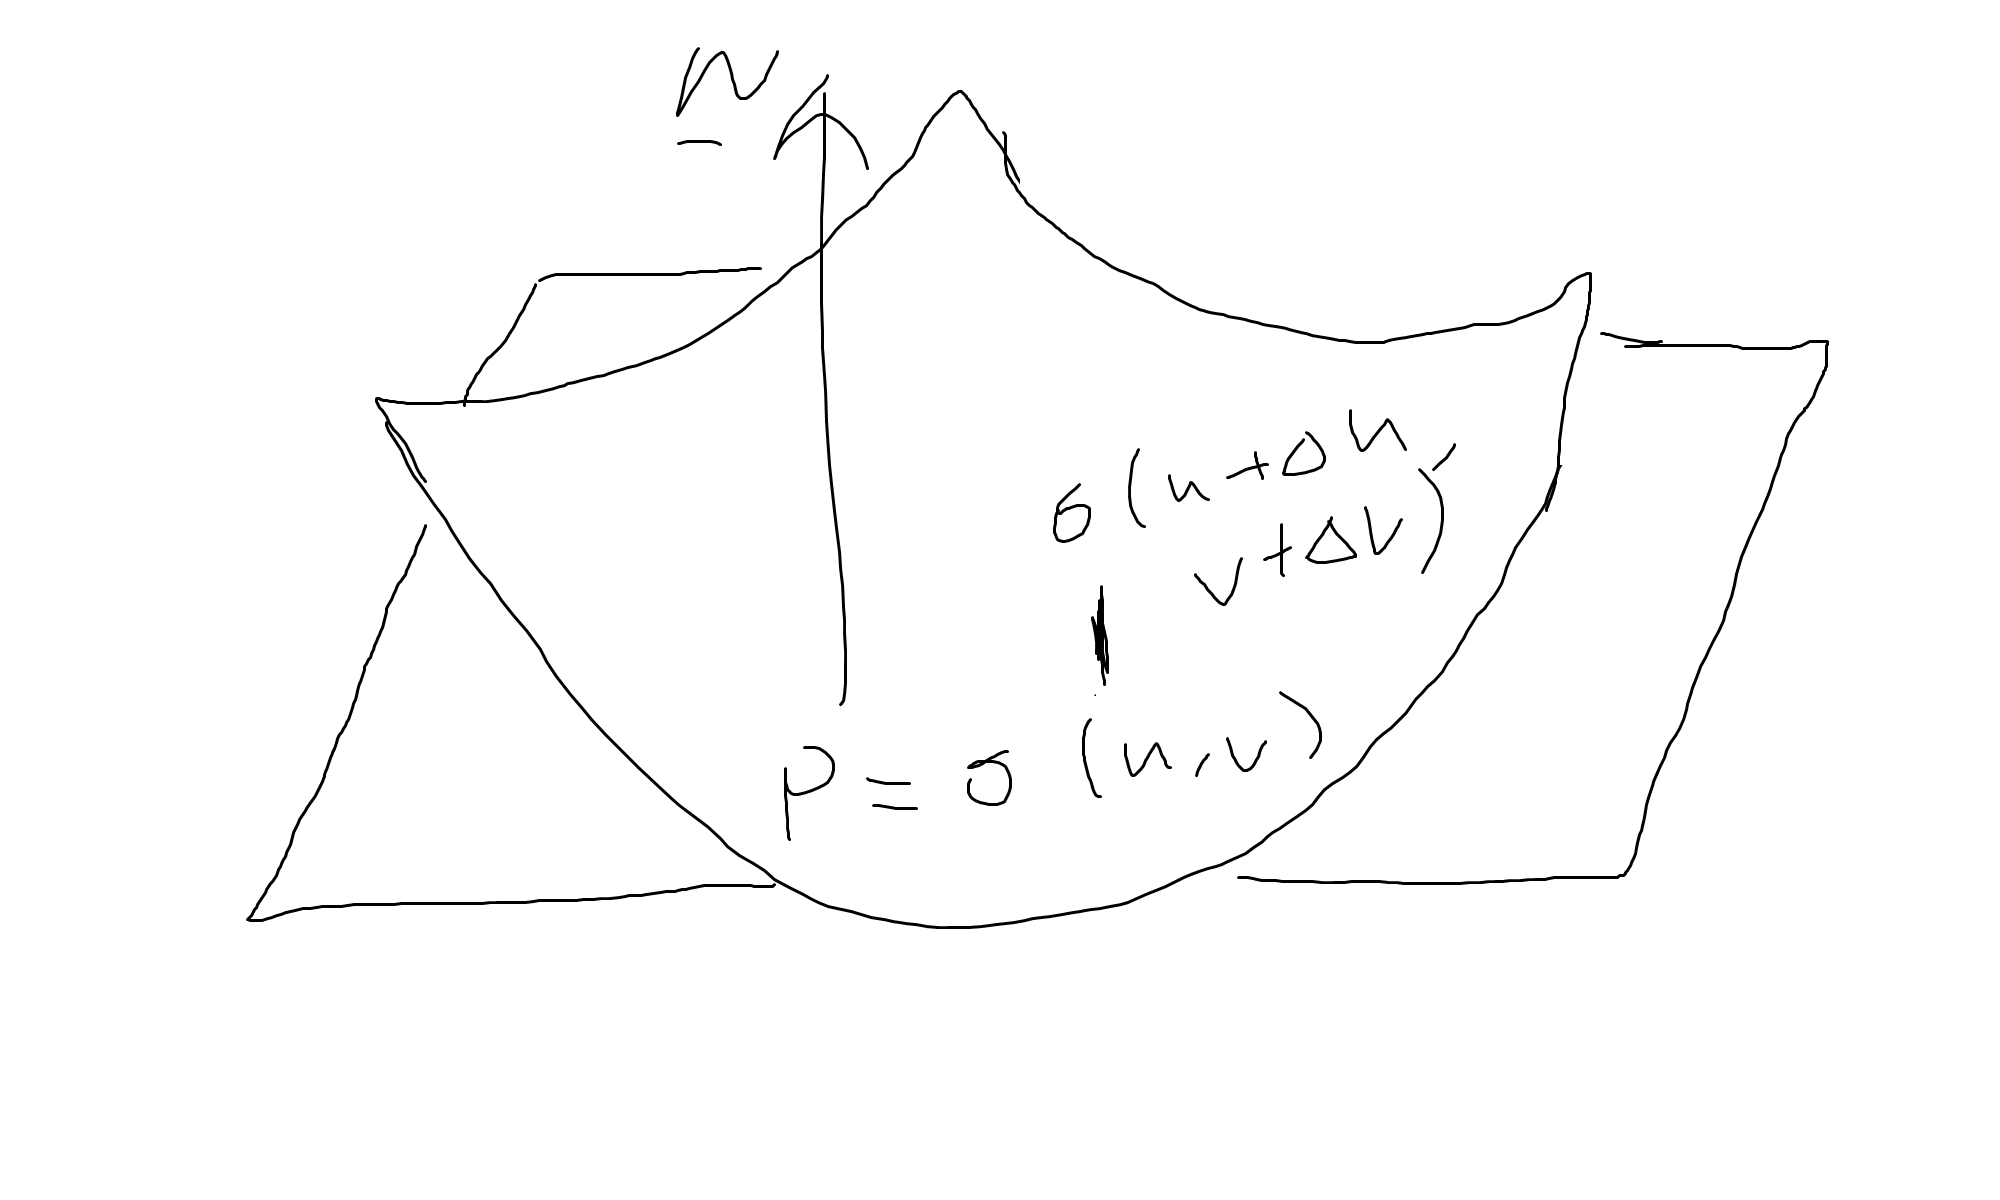
\includegraphics[scale=0.4]{Geometry_24}

Recall
\begin{equation*}
\begin{aligned}
||\sigma(u+\Delta u,v+\Delta v) - \sigma(u,v)||^2 = E(\Delta u)^2 + 2F(\Delta u) (\Delta v) + G(\Delta v)^2 + ...
\end{aligned}
\end{equation*}

\begin{defi}
The second fundamental form on $V$ (for $S$) is
\begin{equation*}
\begin{aligned}
L du^2 + 2M dudv + N dv^2
\end{aligned}
\end{equation*}
with $L,M,N \in C^\infty(N)$ as just defined.
\end{defi}

\begin{defi}
The \emph{Gaussian curvature} $\mathcal{K}$ of $S$ at $P$ is 
\begin{equation*}
\begin{aligned}
\mathcal{K} = \frac{LN-M^2}{EG-F^2}
\end{aligned}
\end{equation*}
If $\mathcal{K}>0$, the second fundamental form is either positive definite or negative definite.\\
On the other hand, if $\mathcal{K}<0$, then the second fundamental form is indefinite.\\
If $\mathcal{K}=0$, the second fundamental form is semi-definite.
\end{defi}

\begin{eg}
The unit sphere has $\mathcal{K}>0$, the Pringle crisp has $\mathcal{K}<0$.
\end{eg}

\begin{rem}
It can be checked, similar to the curves story, that $\mathcal{K}$ does not depend on parameterisation.
\end{rem}

\begin{prop} 7.1\\
Write $\mathbf{N}$ for the unit normal
\begin{equation*}
\begin{aligned}
\frac{\sigma_u \times \sigma_v}{||\sigma_u \times \sigma_v||}
\end{aligned}
\end{equation*}
Then at each point, $\mathbf{N}_u = a \sigma_u + b\sigma_v$, $\mathbf{N}_v = c\sigma_u + d\sigma_v$(*), where
\begin{equation*}\tag{**}
\begin{aligned}
-\left(\begin{matrix}
L & M\\
M & N
\end{matrix}\right) = \left(\begin{matrix}
a & b\\
c & d
\end{matrix}\right) \left(\begin{matrix}
E & F\\
G & H
\end{matrix}\right)
\end{aligned}
\end{equation*}
in particular, $\mathcal{K} = ad-bc$.
\begin{proof}
$\mathbf{N} \cdot \mathbf{N}=1$, so $\mathbf{N} \cdot \mathbf{N}_u = 0$ and $\mathbf{N} \cdot \mathbf{N}_v=0$. So (*) holds for some $a,b,c,d$.
\begin{equation*}
\begin{aligned}
&\mathbf{N} \cdot \mathbf{\sigma}_u = 0 \\&\implies \mathbf{N}_u \cdot \mathbf{\sigma}_u + \mathbf{N} \cdot \mathbf{\sigma}_{uu} = 0 \\
&\implies \mathbf{N}_u \cdot \mathbf{\sigma}_u = -L
\end{aligned}
\end{equation*}
similarly, $\mathbf{N}_u \cdot \mathbf{\sigma}_v = -M = \mathbf{N}_v \cdot \mathbf{\sigma}_u$, $\mathbf{N}_v \cdot \mathbf{\sigma}_v = -N$
dot (*) with $\sigma_u$ and with $\sigma_v$, we get
\begin{equation*}
\begin{aligned}
-L = aE+bF,\\
-M = cE+dF
\end{aligned}
\end{equation*}
\begin{equation*}
\begin{aligned}
-N=aF+bG,\\
-N=cF+dG
\end{aligned}
\end{equation*}
which is (**). Take the determinants to obtain
\begin{equation*}
\begin{aligned}
\mathcal{K} = \det \left(\begin{matrix}
a & b\\
c & d
\end{matrix}\right).
\end{aligned}
\end{equation*}
\end{proof}
\end{prop}

\begin{thm} 7.2\\
Suppose for a $\sigma:V \to U \subset S \subset \R^3$. The first fundamental form $du^2+G(u,v)dv^2$ ($G \in C^\infty(v)$). Then
\begin{equation*}
\begin{aligned}
\mathcal{K} =\frac{-(\sqrt{G})_{uu}}{\sqrt{G}}
\end{aligned}
\end{equation*}
\begin{proof}
To show $K=-\frac{(\sqrt{G}_{uu}}{\sqrt{G}}$ when the first fundamental form (Riemannian metric) is of the form $du^2 + G(u,v) dv^2$, set $e=\sigma_u$, $f=\frac{\sigma_v}{\sqrt{G}}$, $\mathbf{N} = e \times f$ an orthonormal basis of $\R^3$ depending on $(u,v)$ ($\sigma(u,v)$ is a parameterisaion as before).

$e\cdot e=1 \implies e \cdot e_u = 0 \implies e_u = \alpha f + \lambda_1 N$.

Similarly, $e_v = \beta f + \lambda_2 N$, $f_u = -\tilde{\alpha} e + \mu_1 \N$, $f_v = -\tilde{\beta} e + \mu_2 N$($+$). Then
$e \cdot f = 0 \implies e_u \cdot f + e \cdot f_u = 0 \implies \alpha = \tilde{\alpha}$. Similar calculation shows $\beta = \tilde{\beta}$. Now
\begin{equation*}
\begin{aligned}
\alpha &= e_u \cdot f\\
&= \sigma_{ii} \cdot \frac{\sigma v}{\sqrt{G}}\\
&= \left[(\sigma_u \cdot \sigma_v)_u - \frac{1}{2} (\sigma_u \cdot \sigma_u)_u \right] \frac{1}{\sqrt{G}}\\
&= 0.
\end{aligned}
\end{equation*}
\begin{equation*}
\begin{aligned}
\beta &= e_v \cdot f\\
&= \sigma_{uv} \cdot \frac{\sigma v}{\sqrt{G}}\\
&= \frac{1}{2} G_u / \sqrt{G}\\
&= (\sqrt{G})_u
\end{aligned}
\end{equation*}
Also from $(+)$, 
\begin{equation*}
\begin{aligned}
\lambda_1 u_2 - \lambda_2 u_1 \\
&= e_u \cdot f_v - e_v \cdot f_u \\
&= (e \cdot f_v)_u - (e \cdot f_u)_v\\
&= -\beta_u\\
&= -(\sqrt{G})_{uu}.
\end{aligned}
\end{equation*}

From Proposition 7.1,
\begin{equation*}
\begin{aligned}
\mathbf{N}_u \times \mathbf{N}_v &= (ad-bc) \sigma_u \times \sigma_v\\
&= \mathcal{K} \sigma_u \times \sigma_v\\
&= \mathcal{K} \sqrt{G}(e \times f)
\end{aligned}
\end{equation*}
So by VC identities
\begin{equation*}
\begin{aligned}
K\sqrt{G} &= (\mathbf{N}_u \times \mathbf{N}_v) \cdot (e \times f)\\
&= (\mathbf{N}_u \cdot e) (\mathbf{N} \cdot f) - (\mathbf{N}_u \cdot f) (\mathbf{N}_v \cdot e)
\end{aligned}
\end{equation*}
But
\begin{equation*}
\begin{aligned}
(N\cdot e)_u = 0 = N_u \cdot e + N \cdot e_u.
\end{aligned}
\end{equation*}
So the above equals
\begin{equation*}
\begin{aligned}
(N \cdot e_u) (N \cdot f_u) - (N \cdot f_u) (N \cdot e_v) &= \lambda_1\mu_2 - \lambda_2 \mu_1 \ -(\sqrt{G})_{uu}
\end{aligned}
\end{equation*}
So done.
\end{proof}
\end{thm}

\begin{defi}
An \emph{Abstract smooth surface} $S$ is a metric space (or Hausdorf topological space) with coflection of homeomorphism called \emph{charts} $\theta_i: U_i \to V_i$ on open $V_i \subset \R^2$, s.t.\\
(i) $S \cup_i U_i$;\\
(ii) $\forall i,j$, $\varphi_{ij} = \theta_i \circ \theta_j^{-1} : \theta_j (U_i \cap U_j) \to \theta_i (U_i \cap U_j)$ is a diffeomorphism.

A \emph{Riemmanian metric} on $S$ is given by a Riemmanian metric on each $V_i = \theta_i(U_i)$ subject to compatibility condition
\begin{equation*}
\begin{aligned}
\left<d\varphi_P(\mathbf{a}),d\varphi_P(\mathbf{b})\right>_{\varphi(P)} = \left<\mathbf{a},\mathbf{b}\right>_P
\end{aligned}
\end{equation*}
where $\varphi = \varphi_{ij}$, $\mathbf{a},\mathbf{b} \in \R^2$.
\end{defi}

Then length, areas, energy, geodesics, etc are all well-defined on $S$ via charts and first fundamental form $E,F,G$ using formulae as before.

It can be shown that for all $P \in S$, we can construct the geodesic polar coordinates $(\rho,\theta) = (u,v)$ around $P$ s.t. metric is $du^2 + G(u,v) dv^2$.

Now we \emph{define} the \emph{curvature} at $P$ to be
\begin{equation*}
\begin{aligned}
\mathcal{K} = -\frac{(\sqrt{G}_{uu}}{\sqrt{G}}.
\end{aligned}
\end{equation*}

\begin{eg}
(i) $\R^2$ with $du^2+dv^2$.\\
(ii) $S^2 \subset \R^3$ embedded surface -- Q3 sheet 3.\\
(iii) $D$ unit in $\R^2$ with $\frac{4(dx^2+dy^2)}{(1-x^2-y^2)^2}$ isometric to $H$ with $\frac{dx^2 + dy^2}{y^2}$.

N.B. \\
$\bullet$ just one char suffices for (i) and (ii);\\
$\bullet$ hyperbolic plane \emph{cannot} be realized as embedded surface in $\R^3$ (theorem of Hilbert).

(i) $dx^2+dy^2$, $G=1$ shows that $\mathcal{K} = 0$.\\
(ii) $S^2 \subset \R^3$ -- exercise Q1 Sheet 3. Use spherical polars (fix radius $=1$), get
\begin{equation*}
\begin{aligned}
& \sigma(\rho,\theta) = (\sin \rho \cos \theta, \sin \rho \sin \theta, \cos \rho),\\
& d\rho^2 + \sin^2 \rho d \theta^2
\end{aligned}
\end{equation*}
(First fundamental form). $\sqrt{G} = \sin \rho$, $\mathcal{K} \equiv 1$.\\
(iii) Hyperbolic disc. Change $x,y$ to Euclidean polars $(r,\theta)$. Then
\begin{equation*}
\begin{aligned}
\frac{4(dx^2+dy^2)}{(1-(x^2+y^2))^2} = \frac{4(d\rho^2 + \rho^2 d\theta^2}{(1-\rho^2)^2}
\end{aligned}
\end{equation*}
Let $\rho=2\tanh^{-1} r$. Hyperbolic metric becomes
\begin{equation*}
\begin{aligned}
d\rho^2 + \sinh^2 \rho d\theta^2,\\
\sqrt{G} = \sinh \rho
\end{aligned}
\end{equation*}
So $\mathcal{K} \equiv -1$.
\end{eg}

\emph{Triangulations} make sense for abstract surfaces $S$ too when $S$ is compact.

Set $e(S) = F-E+V$ the Euler Number.

\begin{thm} (Gauss-Bonnet)\\
(1) If the sides of triangle $\Delta = ABC$ are geodesic segments, then
\begin{equation*}
\begin{aligned}
\int_{\Delta} K dA = (\alpha+\beta+\gamma) - \pi
\end{aligned}
\end{equation*}
where $\alpha,\beta,\gamma$ are angles, $dA = \sqrt{EG-F^2} dudv$ in each chart. So\\
(2) If $S$ is compact, then
\begin{equation*}
\begin{aligned}
\int_S K dA = 2\pi \cdot e(S).
\end{aligned}
\end{equation*}
this is called the global Gauss-Bonnet.
\end{thm}

\end{document}